%%%%%%%%%%%%%%%%%%%%%%%%%%%%%%%%%%%%%%%%%%%%%%%%%%%%%%%%%%%%%%%%%%%%%
%%                                                                 							%%
%%		Trabajo Fin de Máster.			                       				%%
%%		Conciliación de Conceptos Formales en Contextos Semánticos.	%%
%%		Jesús Giráldez Crú									%%
%%                                                                 							%%
%%%%%%%%%%%%%%%%%%%%%%%%%%%%%%%%%%%%%%%%%%%%%%%%%%%%%%%%%%%%%%%%%%%%%

%%  Include con la definicion de estilos por el usuario
%%%%%%%%%%%%%%%%%%%%%%%%%%%%%%%%%%%%%%%%%%%%%%%%%%%%%%%%%%%%%%%%%%%%%

\input definl

%%  Paqueteria necesaria de fabrica
%%%%%%%%%%%%%%%%%%%%%%%%%%%%%%%%%%%%%%%%%%%%%%%%%%%%%%%%%%%%%%%%%%%%%
\usepackage{hyperref}
\usepackage{palatino}
\usepackage[dvips]{graphicx} 	% para importar combinados latex
\usepackage{color}          		% para importar dibujos coloreados
\usepackage{rotating}        		% para usar \begin{sideways} que rota tabla 90 grados 
\usepackage{epsfig}          		% para rotar figuras de Xfig  poniendo % \begin{sideways} 
\usepackage{amsmath}         	% para usar matrix y pmatrix environment
\usepackage{stmaryrd}        		% para usar la \bigsqcap
\usepackage{verbatim}        		% para poner salidas de pantallas
%\usepackage{listings}       	 	% para imprimir codigo fuente
\usepackage{shortvrb}
\usepackage{url}
\usepackage{subfigure}

%%  Configuracion de paquetes
%%%%%%%%%%%%%%%%%%%%%%%%%%%%%%%%%%%%%%%%%%%%%%%%%%%%%%%%%%%%%%%%%%%%%
%\renewcommand\lstlistingname{Listado}                   %  default is Listing
%\renewcommand\lstlistlistingname{\'Indice de listados}  %  default is Listings 
%\renewcommand\thelstlisting{\thechapter .\arabic{lstlisting}} % captionstyle


%\lstset{
%  language=Java,
%  basicstyle=\small,
%  keywordstyle=\bfseries,
%  showstringspaces=false,
%  numbers=left, 
%  numberstyle=\tiny, 
%  stepnumber=1, 
%  numbersep=5pt,
%  frame=single}


%%  Configuraciones varias
%%%%%%%%%%%%%%%%%%%%%%%%%%%%%%%%%%%%%%%%%%%%%%%%%%%%%%%%%%%%%%%%%%%%%
\newcommand{\corregir}{\color{blue}}  	 	% pintar en color azul
\setlength{\parskip}{2ex}              			% despues del parrafo, doble linea


% Para que no aparezcan las cabeceras de las páginas que están en blanco
%%%%%%%%%%%%%%%%%%%%%%%%%%%%%%%%%%%%%%%%%%%%%%%%%%%%%%%%%%%%%%%%%%%%%
\makeatletter 
\def\cleardoublepage{\clearpage\if@twoside \ifodd\c@page\else
  \hbox{} 
  \thispagestyle{empty} 
  \newpage
  \if@twocolumn\hbox{}\newpage\fi\fi\fi} 
\makeatother

%%  Cortes de palabras especiales
%%%%%%%%%%%%%%%%%%%%%%%%%%%%%%%%%%%%%%%%%%%%%%%%%%%%%%%%%%%%%%%%%%%%%
\hyphenation{
ejem-plo Algo-ritmo
}


%\includeonly{titulo, prologo,intro,capitulo1}


\begin{document} 

%%  Titulo e Indices
%%%%%%%%%%%%%%%%%%%%%%%%%%%%%%%%%%%%%%%%%%%%%%%%%%%%%%%%%%%%%%%%%%%%%%
\pagenumbering{roman}
\thispagestyle{empty}

{


\thispagestyle{empty}
\begin{center}

\includegraphics[scale=.6]{img/logous}
\end{center}

\vspace*{0cm}
\Large 

\begin{center}

{\normalsize \sc Escuelta Técnica Superior de Ingeniería Informática}

{\large \bf Máster Oficial en Lógica, Computación e\\ Inteligencia Artificial }

\vspace*{1.5cm}

{\sc Trabajo Fin de Máster}


{\LARGE \bf Conciliación de Conceptos Formales \\ en Sistemas de Etiquetado\\ mediante Sistemas MultiAgente}

\end{center} 




\vspace*{0.5cm}
%\vfill

\begin{center}
{\normalsize Autor: \\ {\bf Jesús Giráldez Crú}}
\end{center}

\begin{center}
%{\footnotesize Tutores:}
{\small Tutores: }
\vspace*{0.2cm}
{\small \\  Joaquín Borrego Díaz \\ Gonzalo A. Aranda Corral}
\end{center}

\vspace*{0.5cm}
\vfill
\begin{center}
{\footnotesize Sevilla, 30 de junio de 2011.\\Curso académico 2010/11. Primera Convocatoria}
\end{center}

%
%\hspace*{.5\textwidth}
%\normalsize
%\begin{tabular}{l}
%
%Trabajo Fin de Máster\\
%de Jesús Giráldez Crú \\
%dentro del programa de Máster en \\
%Lógica, Computación 
%e Inteligencia Artificial\\
%
%% para optar al grado de \\
%% 
%% trabajo de investigaciÛn\\
%% 
%% por la Universidad de Sevilla \\
%%  
%\end{tabular} \par
%
%% \vspace{2cm}
%% 
%% \hspace*{.5\textwidth}  
%% \quad Gonzalo Antonio Aranda Corral \par
%% 
%
%\vspace*{-2.9cm}
%
%V. B. Director
%
%\vspace*{4cm}





\newpage
\thispagestyle{empty}
\mbox{ }
\newpage
\thispagestyle{empty}

\newpage
\thispagestyle{empty}

\mbox{ }

\vfill

\begin{flushright}
  \begin{minipage}{9cm}
%\begin{right}
%    \em{``El hombre es inteligente porque tiene manos''}\\ \\Anax·goras 
%\end{right}
%    \em{``Iré a cualquier parte, siempre que sea hacia delante.''}\\ \\ 
%David Livingston.


%{\em Ya veré...}

\end{minipage}
\end{flushright}

\vfill

\newpage
\thispagestyle{empty}
\mbox{ }

}

%! \newpage
%! \chapter*{Agradecimientos}
%! \thispagestyle{empty}
%! 
%! Agradecimientos a todo el personal
%! 
%! \newpage
%! \thispagestyle{empty}
%! \mbox{ }
%! 
%%% Local Variables: 
%%% mode: latex
%%% TeX-master: "../dea"
%%% End: 
  

\clearpage
\pagestyle{plain}
\tableofcontents
\clearpage
\listoffigures

%%  Contenido del trabajo
%%%%%%%%%%%%%%%%%%%%%%%%%%%%%%%%%%%%%%%%%%%%%%%%%%%%%%%%%%%%%%%%%%%%%%
\pagenumbering{arabic}
\pagestyle{fancy}

%\chapter*{Prólogo}
\label{intro:prologo}
\addcontentsline{toc}{chapter}{Prólogo}

	La conciliación es...
\chapter*{Introducción}
\label{intro:intro}
\addcontentsline{toc}{chapter}{Introducción.}

En ocasiones, la búsqueda de información sobre ciertos temas en Internet se convierte en una ardua tarea, debido a que los resultados que encontramos no son demasiado relevantes. Esto se debe a numerosas razones. En general, se puede decir que los parámetros con los que ajustamos la búsqueda no termina de ser los más apropiados para conseguir los resultados que esperamos; bien porque no hemos sabido ajustar correctamente las palabras claves en nuestra búsqueda, y por tanto, los resultados obtenidos versan sobre otros temas distintos; o bien porque, aunque estas palabras claves sí sean relativamente correctas, los resultados obtenidos son más específicos o más generales de lo que buscamos, y por tanto estos resultados tampoco son conveniententes. Desde el punto de vista de búsquedas en contextos \emph{semantizados} \footnote{Se entiende por contextos \emph{semantizados} a aquellos que están marcados con ciertos metadatos semánticos.}, podemos decir más concretamente que si los resultados encontrados no son apropiados, es porque el conocimiento con el que hemos ajustado la búsqueda es incompleto, o incluso incorrecto.

Una posible solución para solventar, o minimizar este problema, podría ser el uso del conocimiento de otros usuarios, además del conocimiento propio del usuario, que ya se dispone. De esta forma, una búsqueda podría ser más completa, ya que el usuario no es el único que aporta conocimiento a los parámetros de dicha búsqueda, sino que éstos se enriquecen con el conocimiento de otros usuarios. Por tanto, el problema se traslada a encontrar relaciones entre usuarios y elegir qué conocimiento será usado para complementar el conocimiento propio de cada usuario.

En este trabajo se propone una solución formal a este problema, en el que se intenta complementar los diferentes conocimientos de cada usuario mediante implicaciones lógicas, que permitan establecer una serie de reglas entre ellos. El conocimiento común que genera un par de usuarios es lo que llamamos {\bf Conciliación de Conocimiento}, como se cita en \cite{algoritmo}. Con este conocimiento conciliado se dispone de una herramienta que puede enriquecer semánticamente cualquier búsqueda. Igualmente, es interesante concebir este conocimiento conciliado desde el punto de vista de la navegación entre usuarios, o entre la información de los mismos, que es, al fin y al cabo, otra forma de buscar información en Internet. Este conocimiento conciliado entre dos usuarios representa un conocimiento aceptado por ambos, ya que está basado en implicaciones lógicas, que aportan un trasfondo formal a este conocimiento. Por tanto, este conocimiento conciliado es equivalente a un contexto común entre ambos usuarios. La navegación semántica entre estos usuarios pasa por un punto intermedio, que es precisamente este conocimiento conciliado.

En este trabajo se propone un método de conciliación del conocimiento en sistemas multiusuario, centrando el caso de estudio en los sistemas de etiquetado. Este método se basa en la utilización de cálculos basados en Análisis Formal de Conceptos (se utilizarán técnicas descritas en \cite{afc}), y ha sido implementado en una estructura de Sistema MultiAgente (SMA) en una plataforma JADE (consutar \cite{jade}).




\section*{Internet, Datos e Información.}
\addcontentsline{toc}{section}{Internet, Datos e Información}

Hoy en día, Internet se ha convertido en una herramienta básica en nuestro día a día. La generación de contenido se produce de una forma masiva, y el volumen de contenido generado crece en forma exponencial; es decir, en cada momento, en Internet se genera una cantidad de contenido mucho mayor que el contenido que se ha generado previamente. Este crecimiento exponencial de Internet es una realidad, y existen algunos problemas que derivan de él, como la gestión de esa cantidad tan grande de contenido.

En los últimos tiempos, este crecimiento del contenido se ha potenciado debido al crecimiento de la Web 2.0, que aporta potentes tecnologías para compartir este contenido con el resto de usuarios (ver \cite{algoritmo} y \cite{mowento}). Ejemplo de ello, es el gran número de herramientas sociales (redes sociales, sistemas de etiquetado, sistemas de compartición de ficheros, etc.), en los que se establece cierta conexión entre los usuarios, y en los que, cada vez más, se integran contenidos multimedia junto con el formato de texto plano que siempre ha existido. El hecho de que estos contenidos multimedia se conviertan en uno de los pilares básicos de esta Web 2.0, trae consigo ciertas consecuencias:

\begin{itemize}
	\item La generación de contenido se vuelve cada vez más masiva, debido al hecho de que el contenido multimedia es más amigable para el usuario. Los avances tecnológicos han propiciado este hecho, debido a que las fronteras de Internet llegan cada vez a más usuarios, y las velocidades de acceso a éste son cada vez más rápidas, y esto hace viable esta generación tan masiva de este contenido, así como su visualización posterior.
	\item El contenido multimedia es, si cabe, más difícil de gestionar y procesar que cualquier contenido en texto plano. Por una parte, el texto plano responde a unos formatos más restringidos, por lo que se podría considerar casi estándar. Sin embargo, el contenido multimedia se clasifica en diferentes tipos (audio, vídeo, imágenes, etc.), en los que cada tipo se clasifica en numerosos formatos. Por tanto, las tareas de gestión son bastante más complicadas, puesto que hay que enfrentarse a diferentes tareas en función del tipo de contenido y del formato del mismo. Por otra parte, el procesado de este contenido también es más complicado. Una búsqueda en un texto plano es, a grosso modo, una tarea de coincidencia de cierta secuencia de caracteres; aunque hoy en día, estas tareas son mucho más complejas que esa simple idea. Sin embargo, en cualquier caso, es una tarea con un coste computacional bajo, y por tanto, rápida. En cambio, en el ámbito del contenido multimedia esta tarea es mucho más complicada. Un símil equivalente podría ser buscar cierta forma en una imágen, cierto sonido en un audio o cierto fotograma en un vídeo. Estos ejemplos son casos de estudio actualmente, y la carga computacional de ellos es de un orden muy superior que el ejemplo de búsqueda en texto plano. En conclusión, el procesado de este contenido es más complicado.
\end{itemize}

Otra característica de estas herramientas 2.0 es la posibilidad de relación social que la propia herramienta ofrece al usuario para que se relacione con otros usuarios. Al igual que el crecimiento del contenido, se produce también un crecimiento en cuanto al número de relaciones entre usuarios, que cada vez más, van estableciendo relaciones con otros usuarios, lo que, dependiendo del sistema, permite acceder a su contenido, compartir contenido común, etc.

De una forma abstracta, esta idea puede entenderse como un concepto de grafo, en el que se represente todo este contenido, mediante nodos, y todas estas relaciones entre usuarios, mediante aristas. Por una parte, a medida que se produce un crecimiento en cuanto a la generación de contenido, encontraríamos un crecimiento en el número de nodos del grafo. Por otra, el crecimiento de las relaciones sociales en el ámbito de la Web 2.0, equivale a un crecimiento del número de aristas de este grafo abstracto que representa todo el conjunto de la web (o simplificadamente, representa a un sistema concreto: un sistema de etiquetado concreto, una red social concreta, etc.).

En conclusión, el crecimiento de Internet hoy en día lleva consigo:
\begin{enumerate}
	\item Una generación masiva de contenido, en gran parte multimedia.
	\item Un problema de procesado de este contenido, debido al gran volumen de los mismo. Y un problema asociado al contenido multimedia, debido a la propia naturaleza de este contenido.
	\item Un conjunto de relaciones entre usuarios de gran volumen.
\end{enumerate}

Es obvio que un trabajo de procesamiento o gestión sobre este compendio de contenido es inviable si se realiza a nivel global. En esta línea, hablaremos de {\bf datos} cuando, en casos como el anteriormente descrito, se disponga de una gran cantidad de contenido pero que es difícil de procesar, analizar y tratar. Sin embargo, es posible añadir cierta metainformación sobre estos datos, para conseguir que estas tareas se puedan llevar a cabo con relativa viabilidad. Con esta metainformación, todo el contenido se puede clasificar más fácilmente, y esta clasificación posibilita un procesado posterior a nivel global que sea viable en cuanto a tiempos de ejecución o carga computacional. Esta metainformación será, en su mayoría, ciertos metadatos semánticos que se añadan a los datos. En el caso de contenido marcados semánticamente, hablaremos de {\bf información}.






\section*{Motivación y Objetivos.}
\addcontentsline{toc}{section}{Motivación y Objetivos}

En la sección anterior, se introduce la posibilidad del marcado semántico (mediante metadatos añadidos al contenido), para convertir los \emph{datos} en \emph{información}. Una vez hecho esto, las posibilidades de procesado a posteriori de esta información son innumerables.

En este trabajo se propone el uso de los Sistemas de Etiquetado, en los que encontramos información marcada semánticamente, con etiquetas, como se verá en el capítulo~\ref{cap:capitulo3}; para llevar a cabo un procesado semántico con el que obtener un conocimiento conciliado entre varios usuarios. Inicialmente se propone conseguir este conocimiento conciliado por pares de usuarios que formen parte del sistema, si bien, en un futuro se puede ampliar a un concepto superior de conocimiento conciliado global. La principal motivación de este trabajo es encontrar un método de conciliación que sea aplicable a sistemas de etiquetado de este tipo, aunque en un futuro se podría ampliar a otro tipo de sistemas. Estas conciliaciones representan un método de navegación entre usuarios, puesto que el conocimiento conciliado que se obtenga para cada par de usuarios, representará un conocimiento común que ambos usuarios aceptan, y por tanto, puede ser una herramienta útil de navegación entre ellos. En un futuro, este conocimiento conciliado podría ser usado en otras tareas como refinamientos de búsquedas, depuración semántica, etc.

Los principales objetivos de este trabajo son:

\begin{itemize}
	\item Formalizar el conocimiento de los Sistemas de Etiquetado.
	\item Extraer los distintos elementos de AFC de estos sistemas.
	\item Implantar un método de conciliación a escala global para todo el conjunto de alguno de estos sistemas.
	\item Analizar los resultados y proponer soluciones futuras que aporten una funcionalidad clara y útil a estos sistemas.
\end{itemize}





\section*{Solución Propuesta.}
\addcontentsline{toc}{section}{Solución Propuesta}

La solución propuesta es un Sistema MultiAgente (SMA) implementado en JADE (ver \cite{jade}), en el que se extraiga el conocimiento de un caso práctico concreto, y calcule un conocimiento conciliado para este sistema. El caso práctico concreto que utilizaremos será un subconjunto de datos de Delicious (ver \cite{delicious}). En el SMA, un conjunto de agentes, que representan a los usuarios del sistema, negociarán entre ellos para conciliar su conocimiento con otros usuarios, en función de su disponibilidad y de la prioridad que tengan en realizar otras conciliaciones con terceros. A medida que avance la ejecución del SMA, se irán produciendo múltiples conciliaciones de forma paralela, de forma que el conocimiento conciliado sea cada vez mayor; y por tanto, se enriquecerá este conocimiento común. Este conocimiento conciliado será almacenado, de forma que se puedan realizar cálculos o extraer conclusiones posteriormente.

En el capítulo~\ref{cap:capitulo6} se comenta la estructura, componentes y funcionamientos de este SMA. En los capítulos anteriores se comentarán algunas técnicas y herramientas necesarias para llevarlo a cabo, o ciertas formalizaciones previas que justifican el trasfondo formal de este trabajo.






\section*{Estructura de la memoria.}
\addcontentsline{toc}{section}{Estructura de la memoria}

Esta memoria se estructura en varios capítulos, con la siguiente distribución de los temas trabajados:

\begin{itemize}
	\item Capítulo~\ref{cap:capitulo1}. Se presenta el Estado del arte en el que se detalla los diferentes modelos de clasificación de la información en Internet, y se plantean las diferentes problemáticas de cada uno de estos modelos.
	\item Capítulo~\ref{cap:capitulo2}. Se formalizan las nociones mátematicas de Análisis Formal de Conceptos (AFC) que sirven como soporte formal en este trabajo.
	\item Capítulo~\ref{cap:capitulo3}. Se introducen los Sistemas de Etiquetado, que serán los casos de estudio concretos de este trabajo, viendo su estructura y la extracción formal de los conceptos de AFC vistos en el capítulo anterior.
	\item Capítulo~\ref{cap:capitulo4}. Se explica el Algoritmo de Conciliación, que permite conciliar el conocimiento de un par de usuarios.
	\item Capítulo~\ref{cap:capitulo5}. Se describen las características del Conjunto de Datos con el que llevaremos a cabo los procesos de prueba empíricamente.
	\item Capítulo~\ref{cap:capitulo6}. Se explica el Sistema MultiAgente (SMA) que se plantea como solución en este trabajo: comportamiento, estructura y componenentes.
	\item Capítulo~\ref{cap:capitulo7}. Se detallan los resultados obtenidos en una prueba empírica llevada a cabo, y se analizan estos resultados.
	\item Capítulo~\ref{cap:capitulo8}. Finalmente, se comentan las conclusiones obtenidas, así como los puntos de trabajo futuro.
	\item Bibliografía.
\end{itemize}
\chapter{Estado del Arte.}\label{cap:capitulo1}

En este capítulo, se introducirá de forma general el estado del arte sobre la clasificación de los datos y la información en Internet, se introducirán los Sistemas de Etiquetado como herramienta de marcación semántica de ciertos datos, se tratarán los diferentes problemas asociados a esta marcación semántica, y finalmente se introducirá la Conciliación de Conceptos como método formal para encontrar conocimiento común entre usuarios.


\section{Clasificación del contenido en Internet.}

La organización del contenido en Internet se realiza a menudo a través de marcas en el contenido con términos descriptivos, también llamados \emph{palabras clave} o \emph{etiquetas}. Esta organización permite al usuario ciertas tareas futuras como navegación, filtro o búsquedas. Esta forma de organización no es, ni mucho menos, nueva; sin embargo, sus creadores en el ámbito de Internet, le acuñaron el nombre de {\bf etiquetado}, con el que actualmente se conoce, y que está ganando mucha popularidad en Internet.

Históricamente, la asignación de estas palabras claves para la organización de colecciones o librerías ha sido tarea de una persona experta en la materia que, bajo su criterio, es quién elige el conjunto de palabras clave y la asignación de las mismas a los diferentes recursos, como se explica en \cite{rowley}. En cambio, el etiquetado colaborativo permite que cualquier usuario participe en esta tarea, de forma que cada recurso pueda ser etiquetado con palabras claves por cualquier usuario y por cualquier palabra clave que éstos elijan.

En cuanto a sistemas de clasificación de contenido, se van a distiguir dos tipos: taxonomías y folksonomías.

Las taxonomías son sistemas de clasificación de contenido basados en la categorización de los recursos (o de los elementos, en general). Esta definición se puede entontrar en \cite{smith}, \cite{kim} o \cite{golder}. Estas categorías deben formar un conjunto completo\footnote{Entiéndase \emph{completo} para un ámbito concreto.} y disjunto; de forma que todos los recursos tengan una categoría con la que pueda ser categorizado, y que además, se elimine (o en todo caso, se minimice) las posibles ambigüedades entre varias categorías. La única excepción en este conjunto disjunto se produce debido a la posibilidad de establecer una jerarquía en las categorías, de forma que se establezca una especialización de las mismas. Estos sistemas son, por tanto, jerárquicos y exclusivos. 

En la otra cara de la moneda, encontramos otros sistemas no jerárquicos y no exclusivos: las folksonomías, cuya definición está aproximadamente consensuada. Esta definición se puede consultar en  \cite{smith}, \cite{kim}, \cite{golder}, \cite{gruber} o \cite{knerr}. En este tipo de clasificación, cada recurso es marcado con una serie de etiquetas, que aportan a estos recursos una serie de metadatos semánticos. En \cite{smith}, se comentan los distintos sistemas que incorporan folksonomías como herramientas; y se discute las diferentes restricciones de cada uno de ellos: conjunto de etiquetas restringido o abierto, etiquetación a recursos propios o globales del sistema, etc. En \cite{golder}, se explica la diferencia entre estos sistemas y los anteriores, cuya principal diferencia es la opción de trabajar con interesecciones entre las diferentes categorías que aparecen, consiguiendo una mejor organización de los recursos y evitando posibles duplicidades de los mismos.

Esta diferencia hace que estos sistemas de etiquetado se hayan convertido en una herramienta muy útil en gran cantidad de sistemas que funcionan en Internet, gracias a la versatilidad que ofrecen al usuario, y además, al ser una herramienta colaborativa, se gestiona gracias a las aportaciones de todos los usuarios, sin necesidad de que una persona experta se encargue de esta tarea. Prueba del auge de estas herramientas, es el enorme número de trabajos que hay sobre ellos desde diversos puntos de vista, como el análisis (estadístico) de los modelos de etiquetación realizado en \cite{golder}, la recuperación y navegación por la información realizado en \cite{halpin} o \cite{jaschke}, o el análisis de redes sociales realizado en \cite{mika} o \cite{brooks}.


\section{El Etiquetado y la Web Semántica.}

Como se ha comentado en la sección anterior, las folksonomías dotan a cualquier sistema en el que se implanten, de una herramienta colaborativa con la cual organizar el contenido. Además, debido a sus características no jerárquicas y no exclusivas, se evitan problemas derivados de otro tipo de clasificaciones, como las taxonomías. Por último, el carácter colaborativo de estas folksonomías han potenciado su popularidad en la Web 2.0, dónde el usuario es el protagonista y \emph{creador} de la propia web (redes sociales, blogs, sistemas de etiquetado, sistemas para compartir ficheros multimedia, etc.).

Por otra parte, estas folksonomías ofrecen una buena alternativa a la web semántica o las ontologías, como se explica en \cite{golder}. Es cierto que estas opciones generan una mayor cantidad de información semántica referente a los recursos del sistema. En cambio, los sistemas de etiquetado, como las folksonomías generan una información semántica muy pobre, que además es ambigua, como se comenta en \cite{algoritmo} y \cite{golder}; en comparación con un sistema basado en ontologías, por ejemplo. En éste último, el marcado semántico es completo, y el procesado semántico (que es la motivación de este trabajo), sería más fácil.

Sin embargo, el concepto de web semántica puede chocar en algunos aspectos con el carácter colaborativo propio de estas folksonomías de los sistemas de etiquetado. Precisamente, uno de los puntos más enriquecedores de estos sistemas es que la información semántica la generan los usuarios, para ser procesada y/o gestionada por ellos mismos. Si bien no existe una formalización en cuanto a la semantización de la información, el papel que juegan los usuarios es crucial para haber conseguido un desarrollo tran grande (frente a otros sistemas, basados en ontologías por ejemplo, que son propios de otro tipo de casos de estudio).

En cambio, como se introdujo en el capítulo anterior, es necesario cierto procesado de la información, para obtener un mecanismo que formalice la semántica de estos sistemas. Las etiquetas serán los elementos que proporcionen esta formalización.






\section{Sistemas de Etiquetado.}

En \cite{smith}, se tratan diversos Sistemas de Etiquetado y las diferentes características de cada una de sus arquitecturas.

De forma general, diremos que un Sistema de Etiquetado está compuesto por Recursos, Etiquetas y Usuarios. En nuestro caso de estudio, los recursos estarán disponibles para cualquier usuario, de forma que un recurso pueda estar etiquetado por múltiples usuarios. El conjunto de recursos es abierto; es decir, cualquier usuario puede añadir nuevos recursos al sistema, por lo que este conjunto está continuamente creciendo. Igualmente ocurre en el caso del conjunto de etiquetas, de forma que una etiqueta puede ser usada por múltiples usuarios, y cada usuario puede añadir las etiquetas que desee al sistema.

En el capítulo~\ref{cap:capitulo3}, se verá de forma detallada las características de los Sistemas de Etiquetado que se tratan en este trabajo. El sistema elegido ha sido Delicious (ver \cite{delicious}), dónde los recursos son URLs que los usuarios guardan, y las etiquetas son campos de texto plano. De esta forma, una URL puede haber sido introducida en el sistema por dos usuarios distintos, por lo que este recurso es \emph{compartido} para ambos (aunque tengan etiquetas distintas para cada uno de ellos). De igual forma, dos usuarios pueden tener etiquetas comunes (o no), que hayan introducido en el sistema.




\section{El Problema de la Heterogeneidad.}

El Etiquetado lleva consigo un problema implícito: la heterogeneidad semántica. En \cite{golder} se comentan algunos aspectos semánticos y cognitivos sobre el proceso de clasificación. Básicamente, se establecen tres problemas principales: polisemia, sinonimia y variaciones del nivel básico.

La polisemia es el problema que se produce debido a que a una palabra tiene varios significados. Al realizar una búsqueda sobre este término, un sistema no sería capaz de distinguir estos significados diferentes; y por tanto, se obtienen más resultados de los esperados, ya que muchos de ellos pertenecen a alguno de los otros significados del término. Esto deriva en un problema de incorrección, pues se obtienen resultados que no deberían obtenerse. Además, este problema es equivalente al producido por homonimia (en concreto, por homografía).

La sinonimia es el problema que se produce debido a que diferentes palabras tienen el mismo significado. Al realizar una búsqueda sobre alguno de estos términos, el sistema sólo será capaz de devolver aquellos resultados que coincidan con el término con el que se ha hecho la búsqueda, obviando todos los resultados de los otros términos sinónimos a éste. Esto deriva en un problema de incompletitud, pues no se obtienen todos los resultados esperados. Además de la definición de sinonimia en lingüística, este problema es equivalente a otros problemas derivados de la escritura propia del usuario. Por ejemplo, las etiquetas \emph{gato} y \emph{gatos} son sinónimos en la práctica, al igual que \emph{para-leer} y \emph{para\_leer}.

Finalmente, existe un problema derivado de las variaciones del nivel básico. En \cite{tanaka} se explica que el nivel básico asocia un problema que surge al existir diferentes términos que describen un único objeto en el rango desde lo más general a lo más específico; el nivel básico es precisamente el que se asocia mayormente con las interacciones humanas. Por ejemplo, \emph{animal}, \emph{perro} y \emph{dálmata} corresponde a la misma categoría, desde la más general a la más concreta. En el ejemplo anterior, para la mayoría de la gente, el nivel básico se establecería en el término \emph{perro}. Sin embargo, existen algunas variaciones sistemáticas en lo que cada individuo considera el nivel básico. Y estas variaciones plantearían este problema, cuya principal consecuencia es incompletitud, aunque también incorrección.

No hay que olvidar que el proceso de etiquetado es básicamente un proceso de interpretación, en el que cada usuario categoriza el contenido en función de una serie de parámetros personales que, en algunos casos, no corresponden con los parámetros del resto.

En \cite{algoritmo}, se describen los problemas anteriores de una forma más formal, en el ámbito del campo de trabajo de los sistemas de etiquetado. Así pues, se tiene:
\begin{itemize}
	\item Hetereogeneidad del Conocimiento dependiente del Contexto (CDKH): Es la limitación producida debido a que una misma etiqueta se refiera a diferentes términos.
	\item Ambigüedad Clásica (CA): Es la limitación producida por las ambigüedades heredadas del lenguaje natural y la elección del nivel básico (\cite{tanaka}) por parte de cada usuario.
\end{itemize}

Por una parte, CA no representa un problema crítico, puesto que el propio objeto (la URL) puede ayudar a desambiguar el significado del término. De hecho, una contextualización de las etiquetas en forma de grafo, puede ayudar a distinguir estos diferentes significados. Sin embargo, CDKH está asociado a estructuras de conceptos que los usuarios no representan en el sistema, aunque métodos de FCA pueden extraer, y por tanto, este problema debe ser tratado con más cautela, y corregido con métodos formales.

Finalmente, hay que comentar que el problema de CDKH es debido a la finalidad con la que se use cierta etiqueta. En \cite{golder}, se definen diferentes tipos de etiquetas:
\begin{itemize}
	\item Identificación del tema que trata: los temas que la URL trata. Por ejemplo \emph{programación}.
	\item Identificación de lo que es: lo que es exactamente la URL. Por ejemplo \emph{libro} o \emph{artículo}.
	\item Identificación del propietario o el creador de la URL. Por ejemplo \emph{Shakespeare}.
	\item Refinación de las categorías. En ocasiones, ciertas etiquetas se usan para complementar la etiquetación de las ya existente. Por ejemplo, números.
	\item Identificación de características: adjetivos, que son la opinión del usuario sobre la URL. Por ejemplo \emph{gracioso} o \emph{estúpido}.
	\item AutoReferencia: del propio usuario. Por ejemplo \emph{mi-libro}.
	\item Etiquetas de organización: ciertas etiquetas se pueden usar para agrupar ciertas URL con un fin común. Por ejemplo \emph{para-leer} o \emph{trabajo-pendiente}.
\end{itemize}



\section{El Etiquetado y la Conciliación de Conceptos.}

Como se ha visto a lo largo del capítulo, en este trabajo se han elegido las folksonomías, y más concretamente los sistemas de etiquetado, como sistemas en los que existen un entorno semantizado, debido a la semántica que las etiquetas aportan a cada objeto del sistema. 

Se ha elegido esta forma de clasificar debido a las ventajas que presenta frente a otros métodos, como taxonomías u ontologías. Sin embargo, se ha explicado los problemas asociados de heterogeneidad y ambigüedad de los términos.

Debido a estos problemas, se han elegido métodos basados en Análisis Formal de Conceptos (AFC) para minimizar las consecuencias de estas ambigüedades semánticas, y establecer un marco de trabajo formal con el que realizar las diferentes operaciones.

La Conciliación de Conceptos es el proceso por el cual, aplicando técnicas de AFC, se van a extraer conceptos formales de los sistemas de etiquetado, tarea que se realizará para cada usuario. Estos conceptos formales nos permitirán calcular un conocimiento común entre los usuarios, que podrá ser usado posteriormente en diferentes tareas: navegación (semántica) entre usuario, refinamiento de búsquedas (semánticas), etc...
 % Introduccion
\chapter{Análisis Formal de Conceptos.}\label{cap:capitulo2}

En este capítulo se formalizan algunas nociones sobre {\bf Análisis Formal de Conceptos} (AFC), que serán necesarias para comprender algunas de las técnicas que se usan en el trasfondo de este trabajo. Las definiciones básicas en AFC son las de Contexto Formal y Concepto Formal. El adjetivo \emph{formal} se usa simplemente para indicar que existe un trasfondo matemático en ambas definiciones, y por tanto, su significado difiere de aquellos que tienen en el lenguaje natural.

A lo largo de todo el capítulo, se incluirá un ejemplo que ilustre todas las definiciones que se van incluyendo. Se ha escogido un ejemplo de pequeño tamaño, para facilitarle al lector la lectura y comprensión del proceso; así como la representación de los resultados que se van obteniendo. Sin embargo, estas técnicas que var a ser definidas en este capítulo, serán usadas en el desarrollo de este trabajo con muestras de un tamaño mucho mayor; y por tanto, los resultados serán igualmente de mayor tamaño, por lo que será mucho más difícil representarlos gráficamente.

Se recomienda consultar \cite{afc} como recurso bibliográfico, en el que se formaliza las definiciones de \emph{conjunto}, \emph{conjunto ordenado} o \emph{retículos completos}, que utilizaremos a lo largo de todo el capítulo. Además, se incluyen las demostraciones de todos los teoremas aquí presentados.

\section{Contextos Formales.}

\begin{defi}
	Un {\bf Contexto Formal} $\K := (G, M, I)$ está compuesto por dos conjuntos $G$ y $M$ y una relación $I$ entre $G$ y $M$ ($I \subseteq \{G \times{M}\}$). Los elementos de $G$ son los {\bf objetos} (formales) y los elementos de $M$ son los {\bf atributos} (formales) del Contexto. La relación entre un objeto $g\in{G}$ y un atributo $m\in{M}$, se expresa como $(g,m)\in{I}$ (o $gIm$), y se lee como ``el objeto $g$ tiene el atributo $m$".
\end{defi}

En el siguiente ejemplo, se ilustra un pequeño contexto sobre peces (objetos) y los hábitats en los que viven (atributos):

\begin{itemize}
	\item Un conjunto de Objetos $G$, que son los peces que forman parte de este contexto: carpa, escatófagus, sargo, dorada y anguila.
	\item Un conjunto de Atributos $M$, que son las posibles características de los objetos anteriores, y que en este ejemplo expresan los posibles hábitats de los peces (que no tienen porqué ser exclusivos): fluvial, litoral y océano.
	\item Una relación $I$, entre $G$ y $M$, expresada en la tabla~\ref{fig:contexto}.
\end{itemize}

\begin{figure}[h]

\centering
{ 
\begin{tabular}{|l|c|c|c|}
\hline
& Océano & Litoral & Fluvial \\
\hline
Sargo &  X  &  X  &    \\ \hline
Dorada &  X  &  X  &    \\ \hline
Carpa &    &    &  X  \\ \hline
Anguila &  X  &  X  &  X  \\ \hline
Escatófagus &    &  X  &  X  \\ \hline
\end{tabular}
}
\caption{Ejemplo de Contexto Formal
\label{fig:contexto}
}

\end{figure}

Como se ve en el ejemplo anterior, un contexto puede ser expresado fácilmente en una tabla de doble entrada, dónde las filas se corresponden con los objetos, y las columnas con los atributos. La relación entre ambos se expresa marcando las casillas correspondientes, de forma que si la casilla de la fila $g$ y columna $m$ está marcada, significa que el objeto $g$ tiene el atributo $m$; es decir que $(g,m)\in{I}$, (o $gIm$). En caso contrario, la casilla quedará sin marcar.

De esta forma, se ve como un objeto puede tener múltiples atributos, y un atributo puede pertenecer a varios objetos.

Denotaremos $\{...\}_{\cal X}$ a un subconjunto de elementos del conjunto ${\cal X}$; es decir que $\{...\}_G$ es un subconjunto de objetos, y $\{...\}_M$ es un subconjunto de atributos.



\section{Intención y Extensión.}

Se definen los conjuntos $A'$ y $B'$, de Intención y Extensión de un Contexto ${\cal K} := (G,M,I)$, como:

\begin{defi}
Para un contexto ${\cal K} := (G,M,I)$ y un conjunto $A\in{G}$ de objetos, se define la {\bf Intención} como el conjunto $A'$; que es precisamente el conjunto de atributos comunes a los objetos de $A$:
\begin{center}
$A' := \{m\in{M}|\ gIm\ \forall{g\in{A}}\}$
\end{center}
\end{defi}

\begin{defi}
Para un contexto ${\cal K} := (G,M,I)$ y un conjunto $B\in{M}$ de atributos, se define la {\bf Extensión} como el conjunto $B'$; que es precisamente el conjunto de objetos comunes a los atributos de $B$: 
\begin{center}
$B' := \{g\in{G}|\ gIm\ \forall{m\in{B}}\}$
\end{center}
\end{defi}

Veamos algunos ejemplos de estas operaciones sobre nuestro contexto ejemplo (figura~\ref{fig:contexto}) para ilustrar estas operaciones:
\begin{itemize}
	\item (1): $\{\ fluvial,\ oc\acute{e}ano\ \}'_M\ =\ \{\ anguila\ \}_G$
	\item (2): $\{\ carpa,\ sargo\ \}'_G\ =\ \emptyset_M$
	\item (3): $\{\ escat\acute{o}fagus,\ sargo\ \}'_G\ =\ \{\ litoral\ \}_M$
\end{itemize}

El ejemplo (1) es un ejemplo de extensión de atributos, mientras que los ejemplos (2) y (3) son ejemplos de intención de objetos.







\section{Conceptos Formales.}

\begin{defi}
Un {\bf Concepto Formal} de un Contexto ${\cal K}:=(G,M,I)$ es un par $(A,B)$ con $A \subseteq G$, $B \subseteq M$, tal que $A' = B$ y $B' = A$, dónde $A'$ y $B'$ son respectivamente la extensión y la intención del concepto $(A,B)$.
\end{defi}

Veamos algunos ejemplos para identificar qué es y qué no es un concepto sobre el contexto de nuestro ejemplo (figura~\ref{fig:contexto}):
\begin{itemize}
	\item (1): $ (\{sargo,\ dorada,\ anguila\}, \{litoral,\ oc\acute{e}ano\}) $ es un concepto; porque:
	\begin{itemize}
		\item $\{sargo,\ dorada,\ anguila\}'\ =\ \{litoral,\ oc\acute{e}ano\}$
		\item $\{litoral,\ oc\acute{e}ano\}'\ =\ \{sargo,\ dorada,\ anguila\}$
	\end{itemize}
	\item (2): $ (\emptyset_G,\ \emptyset_M) $ no es un concepto; porque:
	\begin{itemize}
		\item $ \emptyset_G'\ =\ M\ \neq\ \emptyset_M $
	\end{itemize}
	\item (3): $ (G,\ \emptyset_M) $ es un concepto; porque:
	\begin{itemize}
		\item No existe ningún atributo común a todos los objetos; es decir:
		\item $ G'\ =\ \emptyset_M $
		\item $ \emptyset_M'\ =\ G $
	\end{itemize}
	\item (4): $ (\emptyset_G,\ M) $ no es un concepto pues:
	\begin{itemize}
		\item Aunque $ \emptyset_G'\ = M $,
		\item se tiene $ M'\ =\ \{anguila\}\ \neq\ \emptyset_G $
	\end{itemize}
\end{itemize}

Los ejemplos (1) y (3) son conceptos porque la extensión del subconjunto de atributos es precisamente el subconjunto de objetos, y la intención del subconjunto de objetos es precisamente el subconjunto de atributos. Los ejemplos (2) y (4) no son conceptos porque no se cumplen alguna de estas dos condiciones.

\begin{defi}
Si $(A_1, B_1)$ y $(A_2, B_2)$ son conceptos de un contexto, $(A_1, B_1)$ es un {\bf subconcepto} de $(A_2, B_2)$ si $A_1 \subseteq A_2$ (o equivalentemente si $B_2 \subseteq B_1$). En este caso, $(A_2, B_2)$ es un {\bf superconcepto} de $(A_1, B_1)$, y se escribe como $(A_1, B_1) \leq (A_2, B_2)$. La relación $\leq$ se llama {\bf orden de jerarquía} (o simplemente {\bf orden}) de los conceptos.
\end{defi}



\section{Retículos de Conceptos.}

En la sección anterior se ha visto que los conceptos pueden ser ordenados jerárquicamente. Esto permite crear un conjunto ordenado de todos ellos.

\begin{defi}
El conjunto ordenado de todos los conceptos de un contexto ${\cal K}:=(G,M,I)$, se denota como ${\cal B}(G,M,I)$, y se llama {\bf retículo de conceptos}.
\end{defi}

En el ejemplo que estamos ilustrando, se obtienen los siguientes conceptos:
\begin{itemize}
	\item $C_0 := (\{anguila, carpa, dorada, escat\acute{o}fagus, sargo\}_G, \emptyset_M)$
	\item $C_1 := (\{anguila, carpa, escat\acute{o}fagus\}_G, \{fluvial\}_M)$
	\item $C_2 := (\{anguila, dorada, escat\acute{o}fagus, sargo\}_G, \{litoral\}_M)$
	\item $C_3 := (\{anguila, escat\acute{o}fagus\}_G, \{litoral, fluvial\}_M)$
	\item $C_4 := (\{anguila, dorada, sargo\}_G, \{litoral, oc\acute{e}ano\}_M)$
	\item $C_5 := (\{anguila\}_G, \{litoral, fluvial, oc\acute{e}ano\}_M)$
\end{itemize}

Y se obtienen las siguientes relaciones de orden entre los conceptos:
\begin{itemize}
  \begin{minipage}[t]{0.3\linewidth} \centering
	\item $C_0 \geq C_1$
	\item $C_0 \geq C_2$
	\item $C_1 \geq C_3$
	\item $C_2 \geq C_3$
  \end{minipage}
   \hspace{0.5cm}
   \begin{minipage}[t]{0.3\linewidth} \centering
	\item $C_2 \geq C_4$
	\item $C_3 \geq C_5$
	\item $C_4 \geq C_5$
   \end{minipage}
\end{itemize}

El retículo de conceptos se puede representar fácilmente en una estructura de grafo, de forma que cada nodo se corresponderá con cada uno de los conceptos que se obtienen del contexto que se representa. Por tanto, habrá tantos nodos como número de conceptos. La relación de orden se expresará en la dirección vertical del grafo, de forma que si un concepto es subconcepto de otro, el superconcepto estará posicionado más arriba que el subconcepto. Por último, y para evitar repeticiones innecesarias en la escritura de los objetos y los atributos, sólo se expresarán una única vez. Los objetos se expresarán en el nodo más bajo posible, de forma que todos los nodos superiores a éste, también contienen a dicho objeto. Los atributos se expresarán en el nodo más alto posible, de forma que todos los nodos inferiores a éste, también contienen a dicho atributo. En la figura~\ref{fig:reticulo}, vemos el grafo obtenido de este retículo de conceptos.

\begin{figure}[t]
\centering
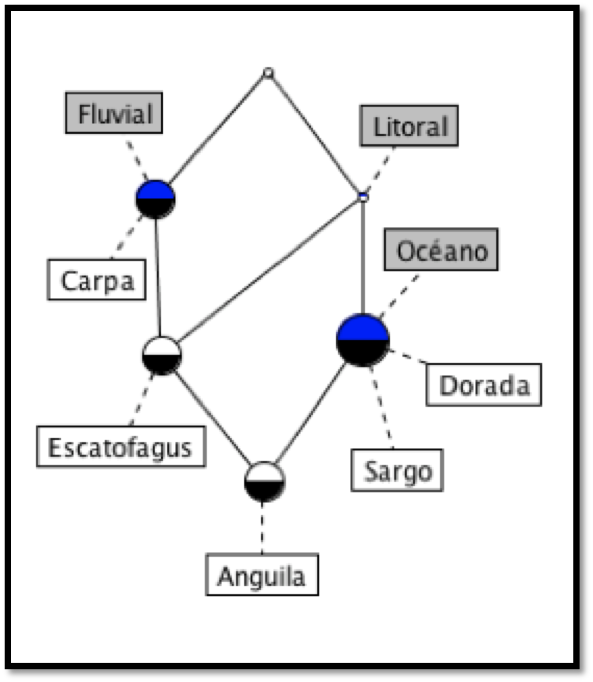
\includegraphics[scale=0.75]{img/2/reticulo}
\caption{Retículo de Conceptos
\label{fig:reticulo}}
\end{figure}



\section{Bases Stem.}

\begin{defi}
Para un contexto ${\cal K}:=(G,M,I)$, Una {\bf implicación} entre atributos es una expresión de la forma $Y_1 \rightarrow{Y_2}$, dónde $Y_1, Y_2 \subseteq M$; es decir, son subconjuntos de atributos.
\end{defi}

El objetivo es obtener un conjunto de relaciones entre los atributos, para que, usando operaciones lógicas, se pueda trabajar con el contexto dado.

A continuación se definen una serie de características sobre las implicaciones. Sea ${\cal L}$ un conjunto de implicaciones; se tiene:
\begin{enumerate}
	\item ${\cal L} \ \models Y \rightarrow{Z}$ ($Y \rightarrow{Z}$ es {\bf consecuencia} de ${\cal L}$) si para todo $T \subseteq M$, si $T$ respeta ${\cal L}$ entonces $T$ respeta $Y \rightarrow{Z}$.
	\item ${\cal L}$ es {\bf cerrada} si contiene a toda implicación $Y \rightarrow{Z}$ que es consecuencia de ${\cal L}$.
	\item ${\cal L}$ es {\bf completo} si toda implicación válida en $(G,M,I)$ es consecuencia de ${\cal L}$:
	\begin{center}
		$(G,M,I) \models Y \rightarrow{Z}\ \ \Longrightarrow{\ \  {\cal L} \ \models Y \rightarrow{Z} }$
	\end{center}
	\item ${\cal L}$ es {\bf no redundante} si ninguna implicación de ${\cal L}$ es consecuencia del resto:
	\begin{center}
		$Y \rightarrow{Z} \in{{\cal L}}\ \ \Longrightarrow{\ \  {\cal L} \backslash \{ Y \rightarrow{Z}\} \not\models Y \rightarrow{Z} }$
	\end{center}
\end{enumerate}

\begin{defi}
	Se define como {\bf Base Stem} al conjunto {\bf completo} e {\bf irredundante} de implicaciones de un contexto ${\cal K}:=(G,M,I)$.
\end{defi}

El problema se reduce, pues, a obtener una Base Stem para un contexto dado. Para ello, se hará uso del cálculo implicacional basado en las Reglas de Amstrong:

\begin{center}
\begin{minipage}[t]{0.3\linewidth} \centering
	$R_1: \frac{}{X\rightarrow{X}}$
\end{minipage}
%\hspace{0.5cm}
\begin{minipage}[t]{0.3\linewidth} \centering
	$R_2: \frac{X\rightarrow{Y}}{X \cup Z \rightarrow{Y}}$
\end{minipage}
%\hspace{0.5cm}
\begin{minipage}[t]{0.3\linewidth} \centering
	$R_3: \frac{X\rightarrow{Y}, Y \cup Z \rightarrow{W}}{X \cup Z \rightarrow{W}}$
\end{minipage}
\end{center}

Con este conjunto de reglas, se puede obtener el siguiente cálculo lógico:

\begin{center}
	${\cal L} \vdash L \Longleftrightarrow{L}$ se prueba mediante las reglas de Amstrong a partir de ${\cal L}$.
\end{center}

\begin{teo}
	Si ${\cal L}$ es un conjunto Stem para un contexto formal ${\cal K}$, entonces ${\cal L}$ proporciona una teoría implicacionalmente completa para ese modelo; es decir:
	\begin{center}
	$ {\cal L} \vdash L \Longrightarrow{ {\cal K} \models L }$
	\end{center}
\end{teo}

\begin{defi}
	$P \subseteq M$ es una {\bf pseudointención} de un contexto ${\cal K}:=(G,M,I)$ si se verifica que:
	\begin{itemize}
		\item $P \neq P''$
		\item Para toda pseudointención $Q \subset P$, se verifica que $Q'' \subseteq P$.
	\end{itemize}
\end{defi}

\begin{teo}
	El conjunto $\{P \rightarrow {P''} | P \mbox{ es pseudointención}\}$ es una Base Stem del Contexto. \\
	En la práctica, únicamente se toman las implicaciones $P \rightarrow {(P''-P)}$, ya que $P \rightarrow {P}$ siempre es válido.
\end{teo}

A cada pseudointención podemos añadirle un atributo de {\bf soporte}, que indica el número de objetos que cumplen esta implicación. Este soporte será un entero mayor o igual a cero.

Veamos en nuestro ejemplo, la traza del algoritmo seguido para calcular las distintas pseudointenciones del contexto. Dado que la definición de pseudointención es recursiva, iniciaremos con el conjunto vacío, e iremos recorriendo los subconjuntos de menor a mayor tamaño. De esta forma, las pseudointenciones calculadas previamente nos pueden ayudar a descartar otras pseudointenciones en el proceso. Por mejorar la visibilidad, únicamente se expresarán las iniciales de los atributos y de los objetos.

\begin{itemize}
	\item $\emptyset_M = G = \emptyset_M$; por tanto, NO.
	\item $\{f\}'' = \{c,e,a\}' = \{f\}$; por tanto, NO.
	\item $\{l\}'' = \{e,s,d,a\}' = \{l\}$; por tanto, NO.
	\item $\{o\}'' = \{s,d,a\}' = \{l,o\}$; por tanto, SÍ.
	\item $\{f,l\}'' = \{e,a\}' = \{f,l\}$; por tanto, NO.
	\item $\{f,o\}'' = \{a\}' = \{f,l,o\}$; sin embargo se tiene que $\{o\}\subset\{f,o\}$, \\ y $\{o\}'' = \{l,o\} \not\subseteq \{f,o\}$; por tanto NO.
	\item $\{l,o\}'' = \{s,d,a\}' = \{l,o\}$; por tanto NO.
	\item $\{f,l,o\}'' = \{a\}' = \{f,l,o\}$; por tanto, NO.
\end{itemize}

Por tanto, la Base Stem obtenida (simplificando las implicaciones) en el ejemplo que hemos seguido a lo largo de todo el capítulo, es:
\begin{itemize}
	\item $(\{oceanico\} \rightarrow {\{litoral\}})$, con soporte 3 (puesto que 3 objetos la cumplen).
\end{itemize}


 % Estado del arte
\chapter{Extracción de Conocimiento en Sistemas de Etiquetado.}\label{cap:capitulo3}

En este capítulo vamos a ver algunas características de los Sistemas de Etiquetado (SE), se enlazarán estas características con los elementos formales que se han visto en el capítulo anterior; y finalmente se comentarán las relaciones entre usuarios desde el punto de vista del Análisis Formal de Conceptos (AFC).

\section{Estructura de los Sistemas de Etiquetado.}

Existen multitud de Sistemas de Etiquetado. En \cite{smith} se citan un gran número de ejemplos, y se explica las diferentes estructuras de cada uno de ellos.

En este trabajo, vamos a centrarnos en Delicious (\cite{delicious}) como Sistema de Etiquetado, y en la folksonomía que el sistema ofrece a partir de la actuación colaborativa de los usuarios. Tomaremos la definición de folksonomía dada en \cite{jaschke}:

\begin{defi}
Una {\bf folksonomía} es una tupla ${\cal F} := (U,E,R,Y)$, dónde:
\begin{itemize}
	\item $U$, $E$ y $R$ son conjuntos finitos, cuyos elementos son, respectivamente, los usuarios, etiquetas y recursos del sistema. En sistemas como Delicious, los recursos son URLs y las etiquetas son campos de texto.
	\item $Y$ es una relación ternaria entre ellos; es decir, $Y  \subseteq \{ U \times{E \times{R}}\}$, cuyos elementos se conocen como etiquetaciones.
\end{itemize}
\end{defi}

Existe un consenso en cuanto a la estructura de este tipo de sistemas, como se puede ver en diferentes definiciones (como en \cite{golder} o \cite{yeung}).

Como se ha comentado en capítulos anteriores, el sistema se va creando gracias a las aportaciones colaborativas de todos los usuarios, que, unido a las características del sistema (no jerárquico y no exclusivo), potencian su popularidad, lo que a su vez genera nuevos usuarios y nuevas aportaciones; el conjunto de datos está en continuo crecimiento. Sin embargo, el problema de heterogeneidad semántica en cuanto a la etiquetación que cada usuario realiza hace que no se produzca un consenso por parte de todos ellos. Por ello, emergen ciertos métodos de resolución de estos conflictos para un posterior procesado de todo el volumen de datos que el sistema posee, que puede llegar a ser muy útil en algunos casos.

En \cite{golder}, se presentan pruebas empíricas sobre la actividad de los usuarios, expresadas en el número de etiquetas que cada usuario usa, la tasa de crecimiento de cada etiqueta, así como el uso de ciertas URLs y la etiquetación de las mismas.

En cuanto al número de etiquetas, existen comportamientos diferentes. Inicialmente, el número de etiquetas por usuario crece en todos los casos. Sin embargo, llegado un punto, existen usuarios que siguen añadiendo nuevas etiquetas, por lo que este número sigue creciendo; mientras otros estabilizan el número de etiquetas que usan, y todas las etiquetaciones que realizan, las hacen con algunas de las etiquetas ya utilizadas.

Por norma general, el uso de una etiqueta va creciendo a lo largo del tiempo, ya que siempre aparecen nuevos usuarios que comienzan a usar esta etiqueta. En el caso de los enlaces es diferente, ya que normalmente emerge un comportamiento en el cual se produce un momento puntual en el cual se producen muchas etiquetaciones de ese enlace de forma masiva, y luego vuelve a descender para seguir unas tasas más pequeñas. Este crecimiento puntual se suele producir o bien al inicio del ciclo de vida de dicho enlace en el sistema, o bien una vez que ha transcurrido un largo período.




\section{Contextos y Conceptos Formales.}

El estudios de los Sistemas de Etiquetado desde el punto de vista formal ha sido un campo de trabajo muy concurrido en los últimos tiempos, y podemos encontrar una gran variedad de propuestas en diversas publicaciones: en \cite{alonso} se propone un método de extensión de atributos; en \cite{yeung} se ofrece un método para minimizar los efectos de hetereogenidad semántica; en \cite{van} se propone un método para convertir en ontologías estas folkonomías; etc...

En el capítulo~\ref{cap:capitulo2} se han introducido las características de los Contextos formales. Estos contextos están formado por un conjunto $G$ de objetos, un conjunto $M$ de atributos, y una relación binaria $I$ entre ambos.

Existe una analogía clara entre estos Contextos formales y los Sistemas de Etiquetado. De hecho, todo Sistema de Etiquetado puede transformarse en un conjunto de Contextos formales. Formalicémoslo:

\begin{teo}
Toda folksonomía ${\cal F} := (U,E,R,Y)$ es transformable en un conjunto de Contextos formales ${\cal K}_i := (G_i, M_i, I_i)$ mediante una función $\gga$, de forma que:
\begin{center}
	$\gga({\cal F}) = \bigcup \limits_{k=1}^{size(U)} {{\cal K}_{\mbox{\scriptsize \emph{k}}}}$
\end{center}

La demostración es trivial estableciendo que $G_i \subseteq R$, $M_i \subseteq E$ e $I_i \subseteq (R \times{E})$. Concretamente está relación binaria $I_i$ se consigue fijando el valor de cada usuario en la relación ternaria $Y$; ésta es la razón por la que se obtienen $size(U)$ contextos diferentes. Los conjuntos $G_i$ y $M_i$ están formados por los objetos y atributos que participan en la relación binaria obtenida anteriormente.
\end{teo}


El teorema anterior nos permite transformar un Sistema de Etiquetado (o un subconjunto completo de éstos) en un conjunto de Contextos Formales. En total se obtienen tantos contextos como usuarios forman parte del Sistema de Etiquetado.

En el caso concreto de este trabajo, cada contexto estará formado por un conjunto de enlaces (objetos) y un conjunto de atributos (atributos), que es precisamente lo que cada usuario aporta de forma colaborativa al sistema de Delicious.

Para cada uno de los contextos anteriores, se puede calcular fácilmente los Retículos de Conceptos que representan el contexto, y las Bases Stem asociadas a éstos.








\section{Relaciones entre usuarios.}

En la sección anterior se ha visto cómo extraer un conjunto de Contextos (formales) de un Sistema de Etiquetado. Cada uno de estos contextos representa el conocimiento de cada usuario dentro del sistema. Es posible establecer una serie de relaciones entre los usuarios, o más bien, entre los contextos de cada uno de ellos. Las más importantes, que son las que utilizaremos en este trabajo, son: Lenguaje común y Conjunto de Objetos comunes.

\begin{itemize}
	\item {\bf Lenguaje común}: Dados dos usuarios y los contextos formales de cada uno de ellos, el lenguaje común es el conjunto de atributos que ambos usuarios tienen. Sean $M_1$ y  $M_2$ los conjuntos de atributos de cada usuario respectivamente; el lenguaje común $\cal{L}$ es precisamente la intesección de estos dos conjuntos:
\begin{center}
	${\cal L} = M_1 \cap M_2$
\end{center}

	\item {\bf Conjunto de Objetos comunes}: Dados dos usuarios y los contextos formales de cada uno de ellos, el conjunto de Objetos comunes es el conjunto de objetos que ambos usuarios tienen. Sean $G_1$ y $G_2$ los conjuntos de objetos de cada usuario respectivamente; el conjunto de objetos comunes ${\cal O}$ es precisamente la intersección de estos dos conjuntos:
\begin{center}
	${\cal O} = G_1 \cap G_2$
\end{center}
\end{itemize}

Además de las dos relaciones anteriores, se pueden establecer otro tipo de relaciones entre usuarios. Se pueden establecer restricciones en las relaciones anteriores para crear nuevas relaciones. Por ejemplo, se puede establecer un lenguaje común reducido entre dos usuarios escogiendo sólo aquellos atributos que, además de pertenecer al lenguaje común, son parte de alguna etiquetación en el mismo enlace para ambos usuarios. Es obvio que este nuevo lenguaje común reducido es bastante más pequeño que aquel en el que no se impone ninguna restricción. Igualmente, se puede crear un conjunto de objetos comunes reducido escogiendo únicamente los enlaces que, además de pertenecer al conjunto inicial de objetos comunes, están etiquetados con una misma etiqueta por ambos usuarios. Igualmente, este último conjunto es mucho más pequeño que el inicial.

Por último, hay que indicar que se pueden establecer tantas relaciones como criterios se quieran inventar. Sin embargo, en este trabajo sólo hemos utilizado las dos anteriores: el Lenguaje común servirá para crear contextos reducidos en los que sólo existan objetos etiquetados con etiquetas pertenecientes a este lenguaje, previo a la conciliación del conocimiento de ambos usuarios; el conjunto de objetos comunes servirá para decidir que pares de usuarios deben realizar conciliación y cuáles no, esto se decidirá en función del tamaño de este conjunto. En este trabajo, únicamente se producirá conciliación entre dos usuarios cuando compartan 3 objetos o más; es decir, cuando esté conjunto de objetos comunes esté formado por 3 o más objetos. 

 % Sistemas de Etiquetado
\chapter{Algoritmo de Conciliación.}\label{cap:capitulo4}

En esta sección, se introduce el Algoritmo de Conciliación basado en Agentes explicado en \cite{algoritmo}, se explicarán los diferentes pasos de la ejecución del algoritmo, así como un análisis de los resultados que aporta y las conclusiones que se pueden extraer de los mismos.



\section{Introducción al Algoritmo de Conciliación.}

A partir del etiquetado propio de un usuario, que refleja su propio conjunto de conceptos sobre los documentos, se pueden obtener diferentes resultados con dos de las principales herramientas del AFC: el retículo de conceptos y las bases Stem; mostrando la heterogeneidad semántica, que se ha descrito en capítulos anteriores. Desde el punto de vista de la navegación por medio de etiquetas, la heterogeneidad semántica hace que esta actividad no asegure el éxito de la misma. De este modo, para asegurar un uso eficiente de las etiquetas de otros usuarios, se debe poner en marcha algún razonador sobre estas etiquetas, cuyo fin es lograr un consenso (también representado por herramientas AFC), que permita la navegación entre estructuras de conceptos diferentes. En este escenario, es importante tratar de delegar estas tareas en agentes inteligentes, como se representa en la figura~\ref{fig:smaGeneral}.

\begin{figure}[t]
\centering
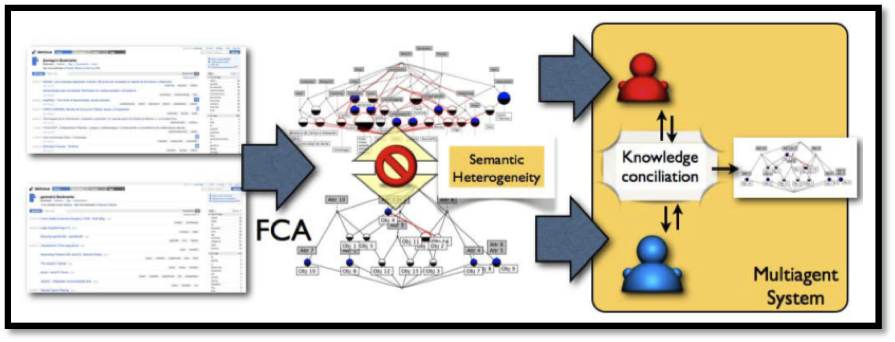
\includegraphics[scale=0.9]{img/4/smaGeneral}
\caption{Conciliación de conceptos a través de retículos de conceptos.
\label{fig:smaGeneral}}
\end{figure}


El Algoritmo original, que se describe detalladamente en \cite{algoritmo}, fue realizado en JADE (consultar más referencias sobre esta herramienta en \cite{jade}). JADE es una herramienta de Sistemas MultiAgente realizada en Java. Dado que en el presente trabajo, el SMA también se ha implementado en JADE, se usará este mismo sistema para la implementación de este algoritmo, de forma que el proceso de integración del algoritmo dentro del SMA sea más sencillo.






\section{Proceso de Conciliación.}

En esta sección se detallan los diferentes pasos (esquematizados en la figura~\ref{fig:algoritmo}) que se llevan a cabo en el algoritmo. Estos pasos son secuenciales; es decir, no se realiza el paso $n$ hasta haber finalizado el paso $n-1$ ($0< n \leq 6$).

\begin{figure}[t]
\centering
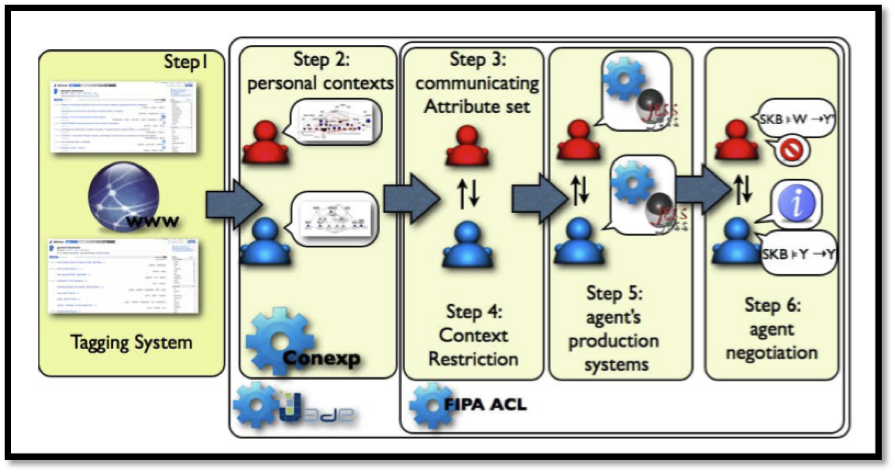
\includegraphics[scale=0.8]{img/4/algoritmo}
\caption{Algoritmo de conciliación
\label{fig:algoritmo}}
\end{figure}


\subsection{Paso 1: Creación de los Agentes.}

En este primer paso de inicialización, se crean a ambos agentes, de forma que éstos representan a los dos usuarios a lo que se les va a conciliar su conocimiento.

Para ello, cada agente deberá conocer los datos del usuario de Delicious al que representa ($id$ y $username$). Igualmente, deberá conocer el nombre del otro agente, con el que realizará la conciliación.

\subsection{Paso 2: Construcción del Contexto Formal y las Bases Stem.}

En este paso, los agente trabajan de forma paralela, sin interacciones entre ellos. Inicialmente, cada agente cargará su propio Conocimiento Base (KB). Este KB se construye a partir de la información de Delicious del usuario al que el agente representa, de forma que los objetos son las enlaces (URLs) y los atributos son las etiquetas asociadas a éstos.

Con estos datos, se construye el Contexto Propio del usuario, del cual se pueden extraer los Conceptos Formales así como las Bases Stem (SB). Para ello, se ha integrado en el algoritmo, la herramienta $Concept Explorer$ de $ConExp$ (ver \cite{conexp} para más referencias), que provee todos los algoritmos de AFC necesarios para realizar estos cálculos.

\subsection{Paso 3: Inicialización del Diálogo.}

En este paso se produce una doble tarea comunicativa, para iniciar el diálogo con el otro agente y comenzar, así, la Conciliación de sus conocimientos.

Por una parte, el agente debe enviar su propio Lenguaje (conjunto de atributos) al otro agente. Por otra, el agente se prepara para recibir el mismo tipo de mensaje del otro agente; es decir, el Lenguaje del otro usuario.

En el proceso de comunicación, se ajustará la intención de cada mensaje a las diferentes performativas FIPA y sus significados. De esta forma, el envío de los lenguajes se realizará con mensajes de performativa tipo {\tt INFORM}.

\subsection{Paso 4: Restricciones del Contexto Formal Propio.}

Después de esta breve comunicación, el agente debe calcular su Contexto Reducido. Para ello, primeramente calculará el Lenguaje Común; es decir, el conjunto de atributos que ambos usuarios comparten, y restringe su Contexto Formal a ese Lenguaje Común. Esta restricción también implica que muchos objetos de este contexto sean eliminados, debido a que no estén etiquetados con ninguna etiqueta de este Lenguaje Común.

Con este nuevo contexto, es decir, el Contexto Reducido propio del agente, éste calculará sus nuevo Retículo de Conceptos y las Bases Stems asociados a él.

\subsection{Paso 5: Creación del Sistema de Producción a partir de las Bases Stem.}

A partir de las Bases Stem calculadas en el paso anterior, el agente únicamente considera aquellas reglas cuyo soporte es mayor que cero. A este conjunto de implicaciones las llamaremos \emph{Bases Stem Kernel} (SKB).

Basándose en las SKB, se creará un sistema de producción, que servirá posteriormente para sugerir a otros agentes los cambios de los objetos que pueden ser aceptados en el contexto común. Este sistema de producción (usado para las nuevas sugerencias de etiquetas) ha sido implementado completamente, por los pocos requisitos del motor de inferencia, y porque no valía la pena integrarlo con otros motores, como Jess4\footnote{\url{http://www.jessrules.com/}} o Drools5\footnote{\url{http://www.jboss.org/drools}}.

\subsection{Paso 6: Negociación del Conocimiento entre Agentes.}

Finalmente, se lleva a cabo este proceso de comunicación y negociación, que se realiza limpiamente en un entorno multiagente. Aunque se podría haber implementado una comunicación cíclica o alternando cambios, mucho más asíncrona; este algoritmo elige la filosofía de multiagentes. La razón es que un escenario normal se compone de KB de diferentes tamaños (de los agentes), por lo que el proceso de comunicación para cada conciliación será diferente.

El proceso de negociación es el siguiente:

\begin{itemize}
	\item La negociación comienza con la creación, por cada agente, de un nuevo contexto (Contexto Común) donde se almacenará el conocimiento común y producirá los resultados de la conciliación. Además, se realiza un envío masivo de todos los objetos (incluidas sus etiquetas asociadas) al otro agente, y espera la respuesta para cada uno de estos objetos. Todos estos mensajes se describen con la performativa {\tt PROPOSE}.
	\item Cuando un agente recibe un objeto, comprueba inicialmente que este objeto satisface todas las implicaciones del SKB propio del agente, y en ese caso, lo incluye en el Contexto Común. Además envía un mensaje de aceptación al otro agente (performativa {\tt ACCEPT\_PROPOSAL}), para que éste también lo incluya en su contexto común.
	\item Si el objeto no satisface alguna implicación del SKB, se introduce en un sistema de producción, creado a partir del SKB (paso 5), y comprueba si alguno de los atributos obtenidos se puede añadir al objeto para que sea aceptado por el SKB. Este nuevo objeto se le envía al otro agente como “objeto nuevo”, reiniciando la negociación sobre dicho objeto. Si el sistema de producción no devuelve ninguna sugerencia, se elimina el objeto y se envía un mensaje de rechazo (performativa {\tt REJECT\_PROPOSAL}) al otro agente para que también lo elimine.
	\item Una vez que se realiza el proceso completo de intercambio de mensajes y  las negociaciones han terminado, los agentes tendrán un Contexto Común, que será igual para ambos agentes. Por tanto, se pueden extraer Conceptos y sugerencias de sus Bases Stem. Éstas representan una conceptualización compartida.
\end{itemize}


\section{Resultados y Conclusiones.}

El algoritmo anterior concilia el Conocimiento asociado a un par de usuarios de algún Sistema de Etiquetado. El método está basado en Análisis Formal de Conceptos, y está diseñado mediante tecnología Multiagente, mediante el cual los agentes colaboran para establecer una representación del conocimiento común, con un nuevo conjunto de etiquetado y nuevos retículos de conceptos.

Hay que indicar que el nuevo Contexto Común obtenido estará formado por el conjunto de atributos comunes (Lenguaje común). Sin embargo, el conjunto de objetos de este contexto estará formado por todos aquellos objetos, de cualquiera de los dos usuarios, que o bien satisfagan todas las implicaciones del Contexto particual de cada usuario, o bien generen nuevos atributos, a partir del Sistema de Producción, para que estas implicaciones acepten esta nueva etiquetación.

Según los datos empíricos aportados en \cite{algoritmo}, se puede concluir que la Conciliación entre dos usuarios genera un Contexto Común dónde el número de atributos (Lenguaje Común) es mucho menor, mientras que el número de objetos es mucho mayor que el de los Contextos Reducidos de cada usuario, ya que se aceptan objetos de ambos.



\begin{figure}[t]
  \begin{minipage}[b]{0.45\linewidth}\centering
	\begin{tabular}{l c c}
	\hline
	Usuario & jborrego & garanda \\ \hline
	Lenguaje & 351 & 137 \\ \hline
	Enlaces & 358 & 536 \\ \hline
	\end{tabular}
  \end{minipage}
\hspace{0.5cm}
   \begin{minipage}[b]{0.45\linewidth}
    \centering
	\begin{tabular}{l c c}
	\hline
	Usuario & jborrego & garanda \\ \hline
	Lenguaje & \multicolumn{2}{c}{19} \\ \hline
	Enlaces & 131 & 114 \\ \hline
	Implicaciones & 11 & 11 \\ \hline
	\end{tabular}
   \end{minipage}
\caption{Contextos antes (izq.) y después (der.) de reducir al Lenguaje Común.}
\label{fig:tabla1}
\end{figure}

\begin{figure}[t]\centering
	\begin{tabular}{l c}
	\hline
	 & Conciliación \\ \hline
	Lenguaje & 19 \\ \hline
	Enlaces & 245 \\ \hline
	Implicaciones & 121 \\ \hline
	\end{tabular}
\caption{Contexto Conciliado.}
\label{fig:tabla2}
\end{figure}

En el experimento realizado en \cite{algoritmo} se usan los usuarios de Delicious de los autores; es decir: {\em garanda}\footnote{http://delicious.com/garanda/} y {\em jborrego}\footnote{http://delicious.com/jborrego/}. Los Contextos iniciales de cada usuario se puede ver en la figura~\ref{fig:tabla1}, así como los Contextos Reducidos obtenidos. Tras aplicar el Algoritmo de Conciliación a estos contextos, se obtiene un Contexto Común, cuyos detalles se adjuntan en la figura~\ref{fig:tabla2}

 % Algoritmo de Conciliacion
\chapter{Conjunto de Datos de Prueba.}\label{cap:capitulo5}

En este capítulo se explica el modelo de Datos utilizado en este trabajo, a partir del cual se van a realizar las distintas Conciliaciones. Para ello, se realizarán una serie de operaciones de reestructuración, tras las cuales, se asegurará la fiabilidad y la consistencia de estos datos.
 
\section{Conjunto de Datos Inicial.}

Como se comentaba en el capítulo~\ref{cap:capitulo3}, el Sistema de Etiquetado elegido en este trabajo es Delicious (\cite{delicious}). En este sistema, los Usuarios que pertenecen al sistema tienen la posibilidad de introducir ciertos Enlaces (objetos) y añadir a éstos ciertas Etiquetas (atributos). Definiremos que una {\bf etiquetación} es el conjunto de etiquetas asignadas a un enlace concreto. De esta forma, los objetos del sistema pueden ser introducidos por múltiples usuarios; sin embargo, la etiquetación para cada uno de ellos puede ser diferente en función del usuario. En el capítulo~\ref{cap:capitulo3} se hace mayor referencia sobre los Sistemas de Etiquetado, aportando conclusiones comentadas en \cite{golder}, \cite{smith} o \cite{van}.

Se define nuestro {\bf Sistema de Etiquetado $S$} como la siguiente tupla :
\begin{center}
$ {\cal F} := <U, E, R, Y> $
\end{center}
cuyos parámetros son:

\begin{itemize}
	\item {\bf U} es el conjunto de Usuarios.
	\item {\bf E} es el conjunto de Enlaces (Objetos del Sistema de Etiquetado).
	\item {\bf R} es el conjunto de Etiquetas (Atributos del Sistema de Etiquetado).
	\item {\bf Y} es una Relación entre U, E y R; de forma que $Y \subseteq (U \times{E \times{R}})$.
\end{itemize}

Según el model anterior, se puede construir fácilmente una Base de Datos (BD) que represente dichos datos. De esta forma, se obtiene las siguientes tablas, pertenecientes a la BD \emph{{\bf conciliacion}}:

\begin{itemize}
	\item Tabla \emph{{\bf users}}: (\underline{int id}, String user, ..., String user\_url). El campo $id$ es la clave primaria, y nos permitirá diferenciar unos usuarios de otros. Existen otros campos que no son relevantes en este trabajo.
	\item Tabla \emph{{\bf links}}: (\underline{int id}, String title, String url, ...). El campo $id$ es la clave primaria, y nos permitirá diferenciar unos enlaces de otros. No se asegura que el campo $url$ sea único, por lo que se deberá arreglar posteriormente. Existen otros campos que no son relevantes en este trabajo.
	\item Tabla \emph{{\bf tags}}: (\underline{int id}, String tag). El campo $id$ es la clave primaria, y nos permitirá diferenciar unas etiquetas de otras. Igualmente, el campo $tag$ es único.
	\item Tabla \emph{{\bf linktags}}: (\underline{int link\_id, int tag\_id,  int user\_id}). La tupla formada por los campos $<link\_id, tag\_id, user\_id>$ conforman la clave primaria, y nos permitirá diferenciar las diferentes etiquetaciones.
\end{itemize}


La recuperación de los datos se ha realizado mediante un proceso de navegación por Delicious, en el que inicialmente se realiza una búsqueda de la etiqueta \emph{\bf haskell}, de forma que pueda ser una etiqueta suficientemente significativa desde un punto de vista semántico. La justificación de la elección de esta etiqueta son las connotaciones que ella misma conlleva: ausencia de polisemia de la etiqueta o ausencia de sinonimía con otras etiquetas; ya que es un término que se da en un campo de actuación muy concreto. Esto nos ayudará a reducir el número de ambigüedades clásicas que ocurren en este tipo de sistemas. Por tanto, el conjunto de datos es un subconjunto en el que todos los objetos están etiquetados con esta etiqueta. Obviamente, el conjunto de datos contiene la etiquetación completa sobre dichos enlaces; así como información sobre estos y la información de los usuarios propietarios de los que se ha obtenido la información.

Hay que indicar que toda la información obtenida se encuentra de forma pública en el sistema Delicious (\cite{delicious}).

Por último, hay que indicar que el conjunto de datos no es completo; ya que no asegura que para cierto usuario, se encuentren todas los enlaces existentes, en los que dicho usuario ha etiquetado con la etiqueta haskell. Igualmente, no se puede asegurar que para cierto enlace, se encuentren todas las etiquetaciones de todos los usuarios que incluyan dicha etiqueta. Sin embargo, el Conjunto de Datos extraído se considera lo suficientemente representativo, al estar inicialmente formado por:
\begin{itemize}
	\item 4327 usuarios.
	\item 3163 enlaces.
	\item 2715 etiquetas.
	\item 57497 tuplas.
\end{itemize}




\section{Operaciones de Reestructuración.}

Como se ha comentado anteriormente, es necesario llevar a cabo una serie de tareas de reestructuración de los datos, con el fin de garantizar la fiabilidad y consistencia del Conjunto, antes de trabajar con ellos. De esta forma, se evitarán ciertos errores estructurales en el futuro. Las diferentes tareas que se llevan a cabo son:

\subsection{Eliminar Etiquetas Irrelevantes.}

\subsubsection{Definición de la tarea.}

La primera tarea de limpieza que se va a llevar a cabo es eliminar todas aquellas etiquetas que sean irrelevantes en el sistema, ya sea por mala escritura, el uso de caracteres ilegibles o, por ejemplo, la etiqueta $haskell$, que al estar presente en todos los enlaces, no es significativa. Para ello, vamos a crear un script que nos permita eliminar una etiqueta (mediante su ID o su nombre). Para ello, se tendrá que:
\begin{itemize}
\item    Eliminar el registro de dicha etiqueta en la tabla tags.
\item    Eliminar todos registros de enlaces-etiquetas-usuarios de la tabla linktags dónde aparezca dicha etiqueta.
\item    Comprobar si tras haber eliminado la etiqueta, algún enlace ha quedado sin etiquetación. Esto representaría un fallo de incoherencia en la BD, ya que dicho enlace seguiría existiendo en la tabla links, pero, sin embargo, no tendría ninguna ocurrencia en la tabla linktags. Por tanto, se realizará esa comprobación, y se eliminarán dichos enlaces.
\end{itemize}

\subsubsection{Implementación de la tarea.}

El Script ha sido realizado en Java. Las fases que se llevan a cabo son:

\begin{enumerate}
\item    Se buscan los enlaces que están etiquetados con la etiqueta que va a ser borrada, junto con el número de etiquetas diferentes con las que está etiquetado.
\item    En caso de que esté número sea 1, entonces sólo está etiquetado con la etiqueta que va a ser eliminada. En este caso, se elimina dicho enlace de la tabla links.
\item    Se eliminan todas las 3-tuplas de enlaces-etiqueta-usuario de la linktags tabla en las que el campo etiqueta sea precisamente la etiqueta que va a ser eliminada.
\item    Finalmente, se elimina la etiqueta de la tabla tags.
\end{enumerate}

Como sistema de seguridad, se usará una copia de seguridad de la base de datos para guardar todos los cambios, de forma que los datos originales siempre sean conservados.



\subsubsection{Resultados y Conclusiones.}

La ejecución de dicha tarea supone:
\begin{itemize}
\item    La eliminación de 45 etiquetas ($tags$).
\item    La eliminación de 101 enlaces ($links$).
\item    La eliminación de 10550 3-tuplas enlaces-etiquetas-usuarios ($linktags$).
\end{itemize}
Por una parte, se ha eliminado la etiqueta “masiva” haskell. Esta etiqueta, al encontrarse en todos los enlaces, no representaba ninguna información adicional. Recuérdese que la base de datos es un subconjunto de enlaces que contienen dicha etiqueta.

Por otra parte, el resto de etiquetas del sistema, son etiquetas marginales; es decir, su relevacia en el sistema es mínima (casi nula). Todas estas etiquetas también pueden ser igualmente filtradas según diferentes criterios al procesarse en un grafo: relevancia de la etiqueta en el sistema (peso del nodo), número de relaciones con otras etiquetas (grado nodal de la etiqueta), u otros criterios que se consideren. Tanto en el caso del peso, cuyo peso es mínimo, o el caso del grado nodal, cuyo grado es mínimo, no pasarían el filtro de procesado de los grafos, por lo que serían eliminadas.

En conclusión, este proceso de limpieza es bueno porque elimina información no relevante antes de generar futuros grafo o trabajar con los datos previos a la conciliación. Sin embargo, no aporta grandes cambios a posteriori, ya que son etiquetas marginales con poca representatividad en el sistema.

\subsection{Eliminar Enlaces iguales.}

\subsubsection{Definición de la tarea.}

Esta tarea tiene como objetivo agrupar aquellos enlaces cuya URL sea idéntica en un único registro; es decir, que si existen dos enlaces con la misma URL pero en dos registros diferentes, se simplificarán en alguno de los dos (cualquiera de ellos), de forma que sólo haya un único registro de dicha URL, y además, se actualizarán todos los registros de $linktags$ de forma que las etiquetaciones (de cualquier usuario y/o cualquier etiqueta) del enlace que va a ser eliminado, pasen a ser etiquetaciones del enlace conservado.

\subsubsection{Implementación de la tarea.}

Se realiza un Script, en Java, con los siguientes pasos:
\begin{enumerate}
\item    Se buscan los pares de enlaces cuyos ID’s son distintos pero sus URL’s son iguales (tabla links).
\item    Para cada par de los anteriores, se buscan todas sus tuplas de etiquetación en linktags.
\item    En caso de que existan dos tuplas iguales (una para cada enlace), se elimina la del enlace de menor ID.
\item    En caso contrario, se actualiza la tupla del enlace de mayor ID con valor del otro enlace.
\item    Se elimina el enlace de menor ID en la tabla links.
\end{enumerate}


\subsubsection{Resultados y Conclusiones.}

Se extraen los siguientes resultados:
\begin{itemize}
\item    Eliminación de 14 enlaces (links).
\item    Eliminación de 3 tuplas (linktags).
\item    Actualización de 552 tuplas (linktags).
\end{itemize}



\subsection{Eliminar Enlaces Equivalentes.}

\subsubsection{Definición de la tarea.}

Esta tarea trata de buscar todos aquellos enlaces equivalentes; es decir, aquellos que se encuentra duplicados en el sistema; y agruparlos en un único enlace. Los enlaces que se encuentran duplicados son aquellos que, siendo el mismo enlace, tienen varias referencias distintas en la BD. Pongamos por ejemplo los siguientes tres enlaces, que son el mismo, pero que en nuestra BD tiene tres referencias diferentes:
\begin{itemize}
  \item http://book.realworldhaskell.org/read
  \item http://book.realworldhaskell.org/read/
  \item http://book.realworldhaskell.org/read/index.html
\end{itemize}

El propósito de esta tarea será encontrarlos automáticamente a partir de una serie de reglas descritas, agruparlos en un único enlaces, y eliminar todas las incongruencias en la BD que produzca esta agrupación.

Se definen las siguientes reglas:
\begin{itemize}
\item    Un enlace que no acaba en ‘/’ y otro con la misma URL añadiendo ‘/’ al final, son el mismo enlace (Ejemplos 1 y 2).
\item    Un enlace que no acaba en ‘/’ y otro con la misma URL añadiendo “/index.html” al final, son el mismo enlace (Ejemplos 1 y 3).
\item    Un enlace que no acaba en ‘/’ y otro con la misma URL añadiendo “/index.php” al final, son el mismo enlace.
\end{itemize}

\subsubsection{Implementación de la tarea.}

El Script automático ha sido realizado en Java. Las fases que se llevan a cabo son:
\begin{enumerate}
\item    Se buscan todos los enlaces del sistema (links).
\item    Para cada enlace que no acabe en ‘/’, se buscan todos aquellos que cumplan alguna de las reglas de corrección descritas anteriormente.
\item    Para cada par de enlace de 1 y enlace de 2 encontrados, se buscan las 3-tuplas enlace-etiqueta-usuario (linktags). Este paso se realiza porque existen usuarios que tienen etiquetados ambos enlaces de la misma forma. Es un paso de verificación para los siguientes pasos:
\item    Si el usuario tiene etiquetados ambos enlaces de la misma forma, se elimina la etiquetación de alguno de los enlaces.
\item    En caso contrario, se actualizan las tuplas para que sólo existan para un enlace, y el otro quede vacío de tuplas.
\item    Finalmente, el enlace que no tiene ocurrencias en la tabla linktags, se elimina de la tabla links.
\end{enumerate}


\subsubsection{Resultados y Conclusiones.}

El resultado de ejecutar esta tarea es:
\begin{itemize}
\item    La eliminación de 19 enlaces (links).
\item    La eliminación de 40 3-tuplas enlace-etiqueta-usuario (linktags).
\item    La actualización de 4086 3-tuplas enlace-etiqueta-usuario (linktags).
\end{itemize}
Es interesante el resultado de esta tarea, ya que partiendo de un total de 46947 tuplas, se han modificado o eliminado 4126 de ellas, lo que supone un 8,79\%.


\subsection{Simplificar etiquetas singular-plural.}

\subsubsection{Definición de la tarea.}

Con esta tarea se pretende corregir todos aquellos errores de etiquetación en los que, para un mismo concepto, existen diferentes etiquetas que lo definen. Un típico error de este tipo es encontrar etiquetas diferentes para el mismo término, escrito uno en singular, y otro en plural. En esta tarea, nos centraremos en buscar y resolver algunos de estos errores singular-plurar (no todos) de una forma autormática.

La regla que usaremos para encontrar dichos errores es una etiqueta y otra que contenga el mismo texto más ‘s’, son la misma etiqueta (singular-plurarl), teniendo que agruparlas en una sola.

Hay que indicar que esta regla no es ni correcta ni completa.
\begin{itemize}
\item    No es correcta porque puede encontrar pares que no se correspondan a singular-plurar. Por ejemplo, las etiquetas C y cs corresponderían con etiquetas diferentes, que no deberían agruparse. Estos casos concretos tendrán que ser tratados como excepciones si se quiere usar este proceso.
\item    No es completa porque no encuentra todos los pares singular-plural. Por ejemplo, las etiquetas process y processes no son encontradas por esta regla y SÍ deberían agruparse al tratarse de la misma etiqueta. Igualmente, estos casos tendrán que ser corregidos manualmente si se quiere usar este proceso.
\end{itemize}

\subsubsection{Implementación de la tarea.}

El Script automático ha sido realizado en Java. Las fases que se llevan a cabo son:
\begin{enumerate}
\item    Se buscan todas las etiquetas del sistema (tags).
\item    Para cada etiqueta, se busca si existe la misma etiqueta añadiéndole una ‘s’ al final.
\item    Para cada par de etiqueta de 1 y etiqueta de 2 encontrados, se buscan las 3-tuplas enlace-etiqueta-usuario (linktags). Este paso se realiza porque existen usuarios que tienen enlaces etiquetados con ambos etiquetas. Es un paso de verificación para los siguientes pasos:
\item    Si el usuario tiene algún enlace etiquetado con ambas etiquetas, se elimina la etiquetación de alguno de las etiquetas.
\item    En caso contrario, se actualizan las tuplas para que sólo existan para una etiqueta, y la otra se elimine.
\item    Finalmente, se elimina la etiqueta (tags) que no tiene ninguna ocurrencia.
\end{enumerate}

\subsubsection{Ejecución de la tarea.}


La ejecución de esta tarea ha encontrado algunas excepciones, como: cs (id=211), iOS (id=614), css (id=687), DS (id=2148), js (id=1636). Estas excepciones, una vez que han sido capturadas, se insertan en la función para que no sean consideradas; se vuelve al estado anterior del sistema y se vuelve a ejecutar la tarea.

\subsubsection{Resultados y Conclusiones.}

El resultado de ejecutar la tarea (una vez corregidas las excepciones) es:
\begin{itemize}
\item    Eliminación de 191 etiquetas (tags).
\item    Eliminación de 1667 3-tuplas de enlace-etiqueta-usuario (linktags).
\item    Actualización de 3756 3-tuplas de enlace-etiqueta-usuario (linktags).
\end{itemize}

Es interesante el resultado de esta tarea, ya que partiendo de un total de 46907 tuplas, se han modificado o eliminado, 5423 de ellas, lo que supone un 11,56\%. 



\subsection{Agrupar Etiquetas Equivalentes.}

\subsubsection{Definición de la tarea.}

Esta tarea tiene como objetivo resolver las diferentes etiquetaciones que, para distintas escrituras de una etiqueta, todas representan el mismo término. Es una tarea que se realizará manualmente, por lo que requiere el conocimiento a priori de los conjuntos de etiquetas que van a ser agrupados.

Por ejmplo, las etiquetas mathematics (id=284), mathematica (id=1918), mathematical (id=1745) y mathemtics (id=2447), serán agrupadas con la etiqueta math (id=66).

\subsubsection{Implementación de la tarea.}

El Script está realizado en Java, y se las fases del proceso son:
\begin{enumerate}
\item    El usuario introduce manualmente el conjunto de etiquetas que van a ser simplificadas, así como la etiqueta que va a agruparlas. Se usará el campo id, que es, además, la clave primaria de la tabla tags.
\item    Para cada par de etiqueta del conjunto y etiqueta “agrupadora”, se buscan las 3-tuplas enlace-etiqueta-usuario (linktags). Este paso se realiza porque existen usuarios que tienen enlaces etiquetados con ambos etiquetas. Es un paso de verificación para los siguientes pasos:
\item    Si el usuario tiene algún enlace etiquetado con ambas etiquetas, se elimina la etiquetación de alguno de las etiquetas.
\item    En caso contrario, se actualizan las tuplas para que sólo existan para una etiqueta, y la otra se elimine.
\item    Finalmente, se elimina la etiqueta (tags) que no tiene ninguna ocurrencia.
\end{enumerate}

\subsubsection{Ejecución de la tarea.}

La ejecución de la tarea se lleva a cabo con los siguientes conjuntos:

\begin{itemize}
\item    Conjunto: $mathematics$ (id=284), $mathematica$ (id=1918), $mathematical$ (id=1745), $mathemtics$ (id=2447), agrupados en {\bf \em math} (id=66).

\item    Conjunto: $to\-read$ (id=681), $unread$ (id=1022), $to\_read$ (id=1030), $2read$ (id=1260), $\_toread$ (id=1418), {\em :$toread$} (id=1515), $*toread$ (id=1530), {\em $to$:$read$} (id=1554), $todo.read$ (id=1612), $toread!$ (id=1627), $toreadlater$ (id=1953), $read\_later$ (id=2326), $later\-read$ (id=2420), agrupados en {\bf \em toread} (id=164).

\item    Conjunto: $*Programming$ (id=603), $programmation$ (id=120), {\em $programaci$Ã$?n$} (id=930), $programming.haskel$ (id=1276), $programmin$ (id=1357), $programing$ (id=1359), $programacao$ (id=1362), $Haskell\_Programming$ (id=1399), $programacion$ (id=1420), {\em $programa$çã$o$} (id=1963), agrupados en {\bf \em programming} (id=4).

\item    Conjunto: $functional\-programming$ (id=131), $functional\_programming$ (id=290), $functional\-language$ (id=423), $Functional.Programming$ (id=491), $programming.functional$ (id=1604), $functionalprog$ (id=1611), \\ {\em $functional$+$programming$} (id=1749), agrupados en {\bf \em functionalprogramming} (id=77).

\item    Conjunto: $e\-book$ (id=1444), $onlinebooks$ (id=1577), $online-book$ (id=1453), $books\-on\-line$ (id=1514), agrupados en {\bf \em ebook} (id=23).

\item    Conjunto: $programming\-language$ (id=234), $programming\_language$ (id=832), $proglanguages$ (id=1330), $proglang$ (id=1352), $prog\_languages$ (id=1591), agrupados en {\bf \em programminglanguage} (id=665).

\item    Conjunto: $langauges$ (id=1670), $lang$ (id=694), $languag$ (id=1033), $languaged$ (id=1586), agrupados en {\bf \em language} (id=5).

\item    Conjunto: $tuto$ (id=1466), agrupados en {\bf \em tutorial} (id=6).

\item    Conjunto: $referencc$ (id=1614), $referenz$ (id=1989), $:reference$ (id=2464), $refs$ (id=2703), agrupados en {\bf \em reference} (id=39).
\end{itemize}

\subsubsection{Resultados y Conclusiones.}

El resultado de esta tarea es:
\begin{itemize}
\item    Eliminación de 52 etiquetas.
\item    Eliminación de 158 3-tuplas de enlace-etiqueta-usuario (linktags).
\item    Actualización de 611 3-tuplas de enlace-etiqueta-usuario (linktags).
\end{itemize}

Es interesante el resultado de esta tarea, ya que partiendo de un total de 45240 tuplas, se han modificado o eliminado, 769 de ellas, lo que supone menos del 1,7\%. Por tanto, no se esperan grandes cambios relevantes por los cambios anteriores. Sin embargo, siempre es útil liberar la BD de información basura.





\subsection{Eliminar Usuarios, Enlaces o Etiquetas sin Etiquetación.}

\subsubsection{Definición de la tarea.}

Con esta tarea se eliminarán todos aquellos registros, tanto de usuarios, etiquetas o enlaces, que tras las operaciones anteriores de limpieza, haya quedado sin etiquetación alguna. Es decir, no tiene sentido, por ejemplo, tener registrado un usuario en el sistema que no tenga ningún enlace etiquetado; por tanto, éste se eliminará. Ídem para los enlaces que no estén etiquetados por ningún usuario, y para las etiquetas que no se usen en ninguna etiquetación.

\subsubsection{Implementación de la tarea.}

Se realiza un Script en Java, con los siguientes pasos:
\begin{enumerate}
\item    Buscar usuarios que no participen en ninguna etiquetación, y eliminarlos.
\item    Buscar enlaces que no pertenezcan a ninguna etiquetación, y eliminarlos.
\item    Buscar etiquetas que no formen parte de ninguna etiquetación, y eliminarlas.
\end{enumerate}


\subsubsection{Resultados y Conclusiones.}

Tras la ejecución de esta tarea, se eliminan:
\begin{itemize}
\item    68 usuarios.
\item    0 etiquetas.
\item    1 enlace.
\end{itemize}

\section{Conjunto de Prueba Obtenido.}

Tras todas las operaciones anteriores, el Conjunto de Pruebas final está compuesto por:
\begin{itemize}
	\item 4259 usuarios.
	\item 3028 enlaces.
	\item 2427 etiquetas.
	\item 45079 tuplas.
\end{itemize}

Además, se añade la siguiente tabla, dónde se almacenarán los resultados de la Conciliación global del sistema:
\begin{itemize}
	\item Tabla \emph{{\bf conciliacion}}: (\underline{int user\_id1, int user\_id2,  int link\_id, int tag\_id,} \\ \underline{int umbral}). La tupla formada por todos los campos de la tabla, conforma la clave primaria, y nos permitirá diferenciar las diferentes etiquetaciones producidas para un Contexto Común de dos usuarios (\emph{user\_id1} y \emph{user\_id2}); usuarios que comparten un número de objetos (enlaces) expresados por \emph{umbral}.
\end{itemize}



 % Modelo de Datos de Prueba
\chapter{Sistema MultiAgente.}\label{cap:capitulo6}
En este capítulo se va a presentar la solución que se ha escogido para llevar a cabo la conciliación de conceptos completa de todo el sistema de etiquetado: un Sistema MultiAgente (SMA).

En este SMA van a convivir un conjunto de agentes encargados de realizar la conciliación por pares de usuarios, como se ha visto en el Algoritmo de Conciliación presentado en el capítulo~\ref{cap:capitulo4}, de forma que al final la ejecución de este SMA, el resultado sea el conocimiento conciliado para todos los usuarios que forman parte del Sistema de Etiquetado.





\section{Introducción a JADE.}

En el capítulo anterior se ha explicado que el Conjunto de Datos de Pruebas está formado por un conjunto de Usuarios, un conjunto de Objetos (Enlaces), un conjunto de Atributos (Etiquetas), y un conjunto de Tuplas \emph{usuario-objeto-atributo}.

Este Conjunto de Datos representa precisamente un Sistema de Etiquetado. Recordemos que en el  caso de este trabajo, como se comentó en el capítulo anterior, se ha seleccionado como conjunto de datos de prueba, un subconjunto de datos de Delicious (\cite{delicious}).

Por otra parte, se dispone de un Algoritmo de Conciliación (descrito en \cite{algoritmo}) que, dado un par de usuarios, calculará el conocimiento conciliado a partir de un Lenguaje Común (o conjunto de atributos comunes) y los Contextos Reducidos (o conjunto de objetos que poseen uno o más atributos de este Lenguaje Común) de cada usuario.

Por tanto, el primer problema es elegir un criterio para seleccionar los pares de usuarios que van a realizar entre ellos un proceso de conciliación. En nuestro caso, el criterio elegido es {\bf el número de objetos (enlaces) comunes} del par. Se ha elegido este criterio porque es una buena forma de obtener un Contexto Común con un número de objetos aceptable, de forma que sea más fácil sacar conclusiones. Otros criterios, como por ejemplo el número de atributos comunes (Lenguaje común), pueden ser considerados en un futuro para analizar el funcionamiento del Algoritmo y extraer otras conclusiones diferentes. En cualquier caso, en este caso, se ha usado este criterio pensando que va a ser con el que más y mejores conclusiones nos aporten los resultados.

La herramienta elegida para modelar el SMA es JADE (\cite{jade}). A continunación se detallan algunas características de este sistema. 

JADE (\emph{Java Agent Developement Framework}) es una herramienta de SMA que ofrece, principalmente, dos servicios. Por una parte, se tiene todo el entorno de computación que permite crear la plataforma dónde convivirán los agentes. Por otra, JADE ofrece todas las herramientas de programación (librerías) para crear los agentes y sus comportamientos en el sistema.

JADE es un software libre (bajo licencia LPGL) desarrollado por Tilab y está completamente realizado en Java, por lo que es posible la utilización de otros paquetes Java para ser incluidos en el código: esto permite que sea un sistema fácilmente extensible y amplio, debido a las innumerables librerías Java que existen. Además, es perfectamente portable, ya que para ser ejecutado, únicamente hace falta que el dispositivo cuente con la JVM (Java Virtual Machine), como cualquier otro programa Java.

En cuanto a la plataforma JADE, ésta se basa en una arquitectura FIPA, que establece estándares para SMA y sus agentes. Se puede consultar \cite{fipa} para más detalles (técnicos) sobre esta arquitectura. Es una plataforma distribuida, por lo que se puede ejecutar en diferentes máquinas. Esto es una característica importante, ya que al ser una plataforma distribuida, la carga de cálculo se reparte entre todas las máquinas que participen en el proceso.

La plataforma del SMA se divide en contenedores, dónde los agentes viven. Todo agente debe vivir en un contenedor, aunque puede haber contenedores dónde no viva ningún agente. Por defecto, la plataforma se inicia con un contenedor genérico principal: \emph{Main Container}. Este contenedor se comporta como un contenedor más, con la única diferencia de que siempre contiene a dos agentes característicos: el AMS (\emph{Agent Management System}) y el DF (\emph{Directory Facilitory}). El agente AMS es un agente que ofrece el servicio de páginas blancas; es decir, registra a todos los agentes del sistema mientras estén vivos. El agente DF ofrece los servicios de páginas amarillas; o lo que es lo mismo, un servicio para encontrar agentes en función de los servicios que éstos ofrecen. Mientras que los registros del AMS son transparentes para el usuario (y por tanto, son fiables); los registros del DF deben ser realizados explícitamente por el usuario (y por tanto, requieren de una comprobación posterior).

La comunicación entre agentes se realiza mediante protocolos estándares (fijados por FIPA; ver \cite{fipa}), permitiendo una separación entre los niveles físicos y lógicos de programación. De esta forma, el emplazamiento real de un agente es transparente para el usuario, ya que el nivel de comunicación se realiza automáticamente por JADE. Por tanto, un agente se comunicará igual con otro que esté en la misma máquina, o en otra máquina de la misma red, o incluso en cualquier otra máquina a la que se pueda conectar por Internet.

En la figura~\ref{fig:arquitecturaJade}, se muestra un pequeño ejemplo de JADE, en el que existe una pequeña red local con cuatro máquinas, dónde se ejecutan distribuidamente dos plataformas JADE. Cada una de ellas, contiene un contenedor principal con los agentes AMS y DF. Además, la Plataforma 1 contiene a los agentes A1 (en el contenedor principal), A2 y A3 ( en el contenedor 1) y A4 (en el contenedor 2). La Plataforma 2 cuenta también con A5 (en el contenedor principal).

\begin{figure}[t]
\centering
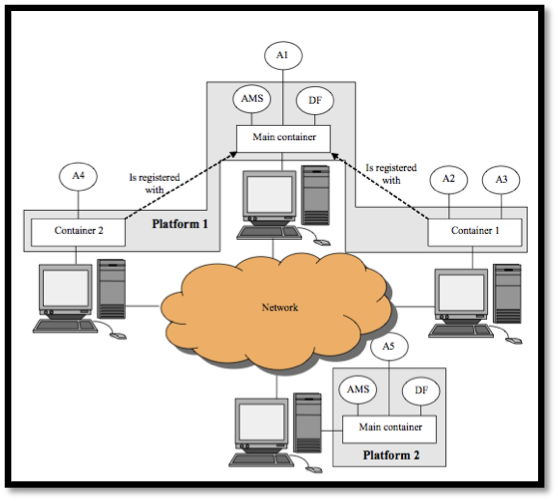
\includegraphics[scale=1]{img/6/arquitecturaJade}
\caption{Ejemplo de Arquitectura en JADE
\label{fig:arquitecturaJade}}
\end{figure}


En cuanto a las librerías que ofrece JADE, hablaremos principalmente de dos elementos: los {\bf agentes} y sus {\bf comportamientos}. Finalmente veremos las características más importantes de la {\bf comunicación}, que es el mecanismo de los agentes para interactuar.

\subsubsection{Agentes.}

Los agentes son cuerpos de ejecución, con unas funciones concretas dentro del sistema, y con capacidad de comunicación con el resto de agentes de la plataforma. En JADE, los agentes no son más que instancias de \emph{jade.core.Agent}.

Cada agente es un ente único dentro del sistema, por lo que tiene un identificador único que le diferencia del resto de agentes. Este identificador (\emph{jade.core.AID}) contiene la descripción única del agente, y tiene la siguiente estructura:

\begin{center}
	$<nickname>@<nombre\_de\_la\_plataforma>:<puerto>/JADE$
\end{center}

El ciclo de vida de un agente consta de tres partes fundamentales:
\begin{itemize}
\item Inicialización: se carga la configuración inicial del agente, y se le prepara para que empiece a funcionar.
\item Acciones: las acciones que un agente realiza se basan en los comportamientos de los que dispone. Cada comportamiento tiene unas tareas concretas, y se modelan independientes para permitir la reutilización de comportamientos por parte de varios agentes.
\item Muerte: significa el fin del agente, por lo que éste desaparece de la plataforma (y se eliminan todas las instancias de éste).
\end{itemize}

\subsubsection{Comportamientos.}


Un comportamiento no es más que una serie de instrucciones con un fin concreto. Ejemplos de comportamientos (muy simples) pueden ser sumar n números, imprimir un mensaje por pantalla, o enviar un mensaje a otro agente. Se pueden hacer comportamientos tan complejos como se puedan realizar en programación Java.

Cada agente dispone de una serie de comportamientos, organizados en dos colas: una cola controla los comportamientos activos, que el agente va gestionando para simular una ejecución paralela de todos ellos; y otra cola de comportamientos bloqueados, que se irán desbloqueando a medida que el agente reciba mensajes (por comunicación).

Un comportamiento genérico es una instancia de la clase \emph{jade.core.behaviours.\-Behaviour} y consta de dos partes:
\begin{itemize}
\item El método \emph{void action()}: son las instrucciones que forma el comportamiento en sí.
\item El método \emph{boolean done()}: indica si un comportamiento ha finalizado (y por tanto, deja de ser parte de la cola de comportamientos activos), o si el comportamiento debe seguir realizándose.
\end{itemize}

Además, existen comportamientos especiales, menos genéricos, como comportamientos que se realizan una sola vez (OneShotBehaviour), comportamientos cíclicos (CyclicBehaviour), periódicos (TickerBehaviour), por máquina de estados (FSMBehaviour), etc…

En la figura~\ref{fig:cicloVidaJade} se explica el ciclo de vida de un agente con sus comportamientos. Inicialmente, el agente se inicializa. Mientras el agente esté vivo, obtiene el siguiente comportamiento que tenga pendiente, y realiza su acción. Comprueba si el comportamiento ha finalizado y actualiza su cola de comportamientos, para coger otro comportamiento y repetir el proceso. Este proceso se repetirá hasta que el agente muera.

\begin{figure}[t]
\centering
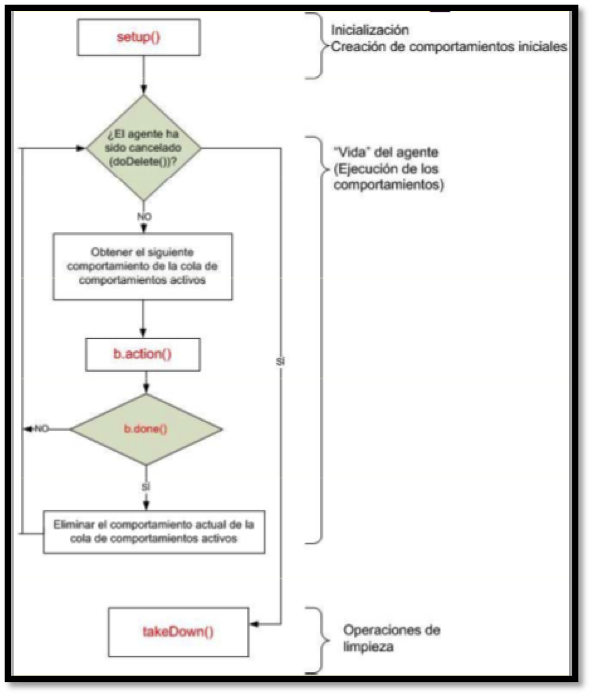
\includegraphics[scale=0.75]{img/6/cicloVidaJade}
\caption{Ciclo de vida de un agente en JADE
\label{fig:cicloVidaJade}}
\end{figure}


\subsubsection{Comunicación.}

La comunicación en JADE se realiza mediante mensajes ACL, que se basan en el estándar FIPA. Estos mensajes son instancias de \emph{jade.lang.acl.\-ACLMessage}. A grosso modo, cada mensaje consta de un receptor y un emisor, un contenido y una intención (tipo del mensaje, según la performativa con la que se mande).

La comunicación es una acción que realiza los agentes, por tanto, debe estar dentro de un comportamiento. Es común encontrar comportamientos de envío de mensajes que se producen una sola vez (OneShotBehaviour) o comportamientos de recepción continua de mensajes (CyclicBehaviour).

Normalmente, la comunicación se implementa mediante protocolos de comunicación. Existen una serie de protocolos que vienen implementados de manera estándar por FIPA. El uso de cualquier protocolo se basa en las directivas de los mensajes, de forma que, dependiendo del tipo de directiva que se reciba, se llevarán a cabo diferentes acciones. JADE implementa algunos protocolos (como FIPA Request, FIPA Query o FIPA ContractNet), y se pueden implementar otros nuevos, ya que JADE da libertad de lenguaje, soportando los lenguajes SL y LEAD (aunque se recomienda SL).

En la figura~\ref{fig:fipaRequest}, se pone el ejemplo del protocolo \emph{FIPA Request}.

\begin{figure}[t]
\centering
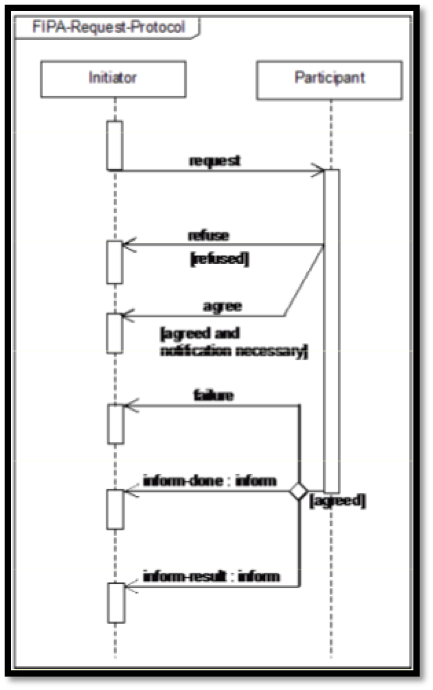
\includegraphics[scale=0.75]{img/6/fipaRequest}
\caption{Protocolo de comunicación FIPA Request
\label{fig:fipaRequest}}
\end{figure}






\subsection{Modelo de la arquitectura JADE.}

Una vez vistas las características generales de JADE en la sección anterior, se va a definir el modelo concreto de la arquitectura JADE aplicado a este trabajo; es decir, hay que definir los contenedores de nuestra plataforma de ejecución, las entidades de agentes, y sus comportamientos:

\begin{itemize}
	\item {\bf Contenedores}: Se usará el contenedor genérico (\emph{Main Container}) que JADE crea por defecto en cualquier ejecución. En este contenedor convivirán todos los agentes necesarios para la ejecución.
	\item {\bf Agentes}: Los agentes del SMA se corresponden con los {\bf Usuarios} del Conjunto de Datos de Prueba. Sin embargo, se establecerá un filtro para crear únicamente a los agentes cuya presencia sea estrictamente necesaria en la ejecución de la Conciliación. La razón para establecer este filtro es reducir el número de agentes existentes en la plataforma, ya que de no hacerse, se crearían tantos agentes como usuarios existan en nuestra base de datos; y este número es bastante alto. La consecuencia de esto sería que, muy probablemente, se diesen errores de ejecución, por desbordamiento en la plataforma debido al excesivo número de agentes en ejecución; y, por tanto, habría que buscar soluciones de implementación mucho más complejas. Sin embargo, con este filtro, se subsana este problema, y se mantiene el mismo comportamiento esperado.
	\item {\bf Comportamientos}: Dado que los agentes se corresponden con los Usuarios de un Sistema de Etiquetado, cada agente debe tener comportamientos para:
	\begin{itemize}
         	\item  Buscar otros usuarios con los que quiera conciliar su conocimiento. 
	         \item  Negociar con otros agentes si ambos están de acuerdo en comenzar una conciliación.
		\item Los comportamientos de conciliación descritos en el Algoritmo de Conciliación del capítulo 4; es decir, comportamientos para calcular el Contexto propio así como comportamientos para dialogar y negociar el conocimiento común.
	\end{itemize}
\end{itemize}







\section{Comportamiento del SMA.}

En esta sección vamos a definir el comportamiento general del SMA, describiendo cada una de las fases por las que el sistema pasa. La estructura del SMA se divide en cuatro partes: {\bf Inicialización del SMA}, {\bf Negociación entre Agentes}, {\bf Proceso de Conciliación}, y {\bf Finalización de la ejecución}.


\subsection{Inicialización del SMA.}

En la fase de Inicialización, se crearán todos los agentes que van a participar en el proceso de Conciliación. Como se ha comentado anteriormente, se va a establecer un filtro a la hora de crear a los agentes, para reducir el número de éstos en la plataforma JADE.

Primeramente, se lanzará la ejecución de la plataforma con un agente Dios (\emph{Agente Control}) cuya objetivo es buscar en el base de datos todos aquellos usuarios que superen el filtro que se elija. Por cada usuario encontrado que valide dicho filtro, se creará una nueva instancia de agente (\emph{Agente Usuario}), se introducirá en la plataforma, se le añadirán los comportamientos oportunos y se lanzará su ejecución.

El filtro que se ha seleccionado es {\bf el número de objetos (enlaces) distintos que componen el Contexto propio} de cada usuario; de forma que si este número no supera cierto umbral, dicho usuario no pasará este filtro y, por tanto, no participará en la ejecución del SMA para realizar el proceso de Conciliación con otros usuarios. Este umbral es precisamente el número de objetos (enlaces) comunes que se ha escogido para realizar la Conciliación entre dos usuarios. La justificación de este umbral es trivial: si dos usuarios concilian su conocimiento cuando poseen cierto número de objetos (enlaces) comunes, es necesario que ambos posean, al menos, ese número de objetos diferentes en su contexto propio.

Cuando un agente comienza su ejecución en la plataforma, debe inicializar las distintas variables con la información relativa al usuario que le corresponde en la base de datos. Igualmente, deberá llevar a cabo un proceso de búsqueda en la base de datos, para ver con que usuarios quiere conciliar su conocimiento. Recordemos que sólo se elegirán a aquellos usuarios que tengan un número de objetos (enlaces) comunes igual o superior a un umbral inicialmente establecido.

Al finalizar esta fase de inicialización, el resultado es una plataforma en la que están conviviendo todos los usuarios que pueden\footnote{Es posible que algunos de los agentes que conviven en la plataforma no participen en ningún proceso de Conciliación con otros usuarios; sin embargo, esto no representa ningún problema de implementación y/o ejecución.} participar en algún proceso de Conciliación con otros usuarios, y todos ellos están ejecutándose con sus comportamientos oportunos, que dependerán de cada usuario, tal y como se detalla en el siguiente apartado.





\subsection{Negociación entre Agentes.}

En esta fase, se establece un protocolo de comunicación entre los agentes, en los que se llevan a cabo paralelamente dos procesos simultáneos:

\begin{itemize}
	\item {\bf Envío de propuestas}: Cada usuario enviará propuestas para conciliar su conocimiento con otros usuarios. Estos usuarios a los que les envía propuestas, han sido calculados previamente en la fase de inicialización. Las propuestas se enviarán según la prioridad con la que quiera conciliarse con otro usuario, de forma que se comenzará enviando propuestas a aquellos usuarios que comparten muchos objetos (enlaces), y será menos prioritario para aquellos con los que comparte un número menor. Si una propuesta recibe una aceptación, ambos usuarios comenzarán el proceso de Conciliación. En caso contrario, el agente buscará otro usuario en su cola de peticiones pendientes, hasta encontrar a un usuario que acepte su petición.
	\item {\bf Recepción de solicitudes}: Cada usuario deberá implementar un procedimiento de recepción de solicitudes, de forma que pueda atender las peticiones que llegan procedentes de otros usuarios. Por norma general, todos los agentes aceptarán las peticiones entrantes que reciban, siempre y cuando no estén ejecutando un proceso de conciliación con otro agente, en cuyo caso no se procesaría dicha solicitud entrante, y por tanto se descartaría.
\end{itemize}

Hay que indicar que un usuario puede iniciar la conciliación de su conocimiento por cualquiera de los dos procesos. Sin embargo, un usuario no puede realizar varias conciliaciones de forma simultánea. Por tanto, si un usuario va a comenzar a conciliar su conocimiento con otro, se deben bloquear los dos procesos anteriores, ya que el usuario no volverá a enviar más peticiones hasta que finalice el proceso de conciliación, e igualmente no podrá atender solicitudes entrantes por la misma razón.

Puede darse el caso de que alguno de los dos procesos descritos anteriormente, bloquee la negociación del otro proceso. Es decir, ambos procesos pueden coexistir y ejecutarse sin problemas. La explicación se da por el paralelismo que ofrece JADE en cuanto a los comportamientos de los agentes; de forma que un comportamiento puede estar bloqueado (esperando que se desbloquee al recibir un mensaje), y al mismo tiempo el agente tener en ejecución otro comportamiento diferente. Por tanto, puede que un agente esté negociando al mismo tiempo con otro tras haberle enviado una propuesta (actuando como iniciador de la negociación), y a la vez con un tercero tras haber recibido una solicitud de éste último (actuando como receptor en la negociación). Se seguirá una estrategia FIFO para solucionar este problema; o lo que es lo mismo, se despachará la negociación que antes se complete, ya sea por el proceso de envío de propuestas o por el proceso de recepción de solicitudes. El otro proceso se bloqueará, y se evitará, de esta forma, que se produzcan dos conciliaciones simultáneas.

En la figura~\ref{fig:transicion}, se adjunta el diagrama de transición de estados de los agentes usuario durante su fase de Negociación y Conciliación, con las fases iniciales y finales de Inicialización y Terminación. Tras la Inicialización, se desarrollan dos comportamientos paralelos de Negociación: el envío de propuestas y la recepción de solicitudes. En este diagrama, se ve gráficamente que es imposible que un agente realice varias conciliaciones simultaneas; ya que se comprueba antes de comenzar cualquier conciliación el valor de {\tt libre}, y en caso de no estarlo, se aborta el proceso.

\begin{figure}[t]
\centering
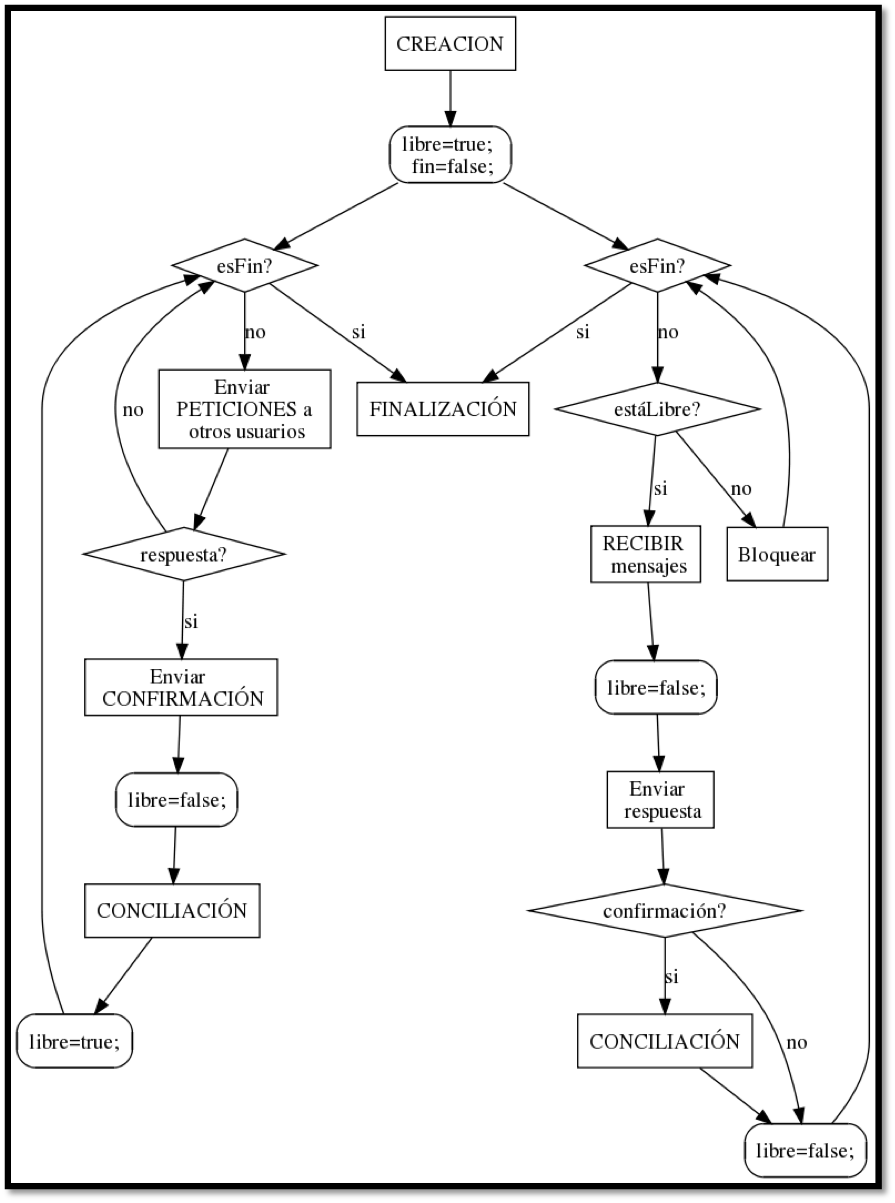
\includegraphics[scale=0.35]{img/6/transicion}
\caption{Diagrama de transición de estados de los Agentes Usuario
\label{fig:transicion}}
\end{figure}


\subsection{Proceso de Conciliación.}

El proceso de Conciliación se llevará a cabo siguiendo el algoritmo descrito en \cite{algoritmo}, que se ha explicado en el Capítulo~\ref{cap:capitulo4}. Por tanto, una vez que dos usuarios han aceptado una negociación, éstos comenzarán esta tarea mediante la cual van a conciliar su conocimiento.

Cuando un agente esté realizando la conciliación con cualquier otro agente, debe bloquear todos sus comportamientos, excepto aquellos que llevan a cabo la conciliación. De esta forma, se evitará que un agente intente negociar conciliaciones simultáneas, restrigiendo este proceso para que únicamente se realice una única conciliación con otro usuario, y que además sea el único proceso que ambos usuarios estén realizando, desde que comience la conciliación hasta que finalice.

En el capítulo~\ref{cap:capitulo4}, se describía las distintas fases del algoritmo. De estas seis fases que constituyen el algoritmo completo, se distinguen dos conjuntos de operaciones, que vamos a separar en el nivel de implementación:

\begin{itemize}
	\item {\bf Cálculos del propio usuario} (Pasos 1-2): En estos pasos se lleva a cabo la inicialización de cada uno de los agentes, y ambos extraen su Contexto personal (de la base de datos), así como sus Retículos de Conceptos y sus Bases Stem. En esta fase, no se produce ningún proceso de comunicación con el otro agente.
	\item {\bf Diálogo entre usuarios} (Pasos 3-6): En esta fase comienza el proceso de diálogo, en el que primeramente se envían y se reciben los Conjuntos de Atributos propios de cada agente (paso 3). Este paso es comunicativo, y además, supone un punto de sincronización en el algoritmo, ya que no se puede avanzar hasta que no se recibe el conjunto del otro usuario. Se continúa calculando el Contexto Reducido (paso 4) y crear un Sistema de Producción a partir de éste (paso 5). En estos pasos no hay comunicación entre agentes. Finalmente, se produce un proceso de Negociación (paso 6), a través de un envío masivo de los objetos de cada usuario, y el procesamiento de cada uno de ellos.
\end{itemize}

Es interesante la distinción de las dos fases anteriores porque: 1) la primera fase es idéntica para todos los procesos de conciliación de un usuario; mientras que la segunda es exclusiva para cada cada conciliación concreta; y 2) en la primera fase no se lleva a cabo comunicación alguna, mientras que la segunda comienza y termina por un acto comunicativo\footnote{Se entiende por {\bf acto comunicativo} al envío o recepción de un mensaje.}.

Por tanto, en el nivel de la implementación, se han realizado dos comportamientos que simulen las dos fases anteriores. La primera vez que un agente realice una conciliación, se creará un comportamiento secuencial de forma que se secuencien ambas fases. Sin embargo, a partir de la segunda conciliación que un usuario realice, la primera fase no será necesario repetirla (los Contextos, Retículos y Bases Stem quedaron guardadas la primera vez que se realizó el proceso), por lo que se llevará a cabo únicamente la segunda fase (pasos 3-6 del algoritmo).

Finalmente, se ha añadido una acción final al algoritmo, que permita almacenar los datos obtenidos en una base de datos (para su posterior procesamiento, extracción de resultados estadísticos, conclusiones, etc...). En esta acción se almacenará el contexto común que se ha obtenido, junto con los datos de ambos usuarios, para saber a quien pertenece. Hay que recordar que con la herramienta ConExp (\cite{conextp}) se puede calcular fácilmente el Retículo de Conceptos y las Bases Stem a partir de este Contexto común, que es el resultado del Algoritmo de Conciliación entre ambos usuarios.



\subsection{Finalización de la ejecución.}

La ejecución global del SMA finalizará cuando todos los usuarios hayan realizado todas las tareas de conciliación que tenían previstas con otros usuarios. Estas tareas se planifican en la fase de Inicialización del SMA, y se almacenan en una cola de peticiones pendientes para cada usuario.

Una vez que un usuario vacíe su cola de peticiones pendientes, enviará un mensaje al Agente Control, y únicamente dejará activo su comportamiento de recepción de solicitudes de otros usuarios. De esta forma, el usuario seguirá activo en la plataforma para atender peticiones entrantes.

El agente Control irá gestionando la recepción de mensajes, cuando cada usuario vacíe su cola de peticiones pendientes. De esta forma, este agente sabrá en todo momento el estado en el que se encuentra cada uno de los usuarios que participan en la plataforma. Hay que recordar que este agente Control es el creador de todos los usuarios, por lo tanto, tiene conocimiento de todos ellos.

Finalmente, el agente Control llevará a cabo una tarea de finalización del sistema una vez que el estado de todos los usuarios sea \emph{terminado}; es decir, cuando haya recibido un mensaje de finalización (por tener vacía su cola de conciliaciones pendientes) de todos los usuarios del SMA.

















\section{Componentes.}

A continuación se detallan los distintos agentes, y sus diferentes comportamientos.

\subsection{Agente Control.}

Este agente es el encargado de comenzar la ejecución del SMA. Únicamente existirá una instancia de él.

En dicho agente se define el {\bf umbral}, que es el número mínimo de objetos (enlaces) comunes que deben tener dos usuarios para realizar una conciliación de su conocimiento. Este umbral es una variable de tipo {\tt entero} mayor o igual a 0. Nótese que cuando el umbral es exactamente 0, equivale a que cada usuario concilie su conocimiento con todos los usuarios con los que comparte 0 o más objetos (enlaces); es decir, con todos los demás usuarios. Por tanto, estableciendo un umbral de 0 unidades, se produciría un proceso de conciliación completo en el sistema: todos con todos. Sin embargo, en nuestro caso, este valor se interpretará de forma excepcional, realizando únicamente la conciliación con aquellos usuarios que no tienen ningún objeto común. En cualquier caso, a nivel de implementación, se ha visto que no tiene sentido realizar conciliaciones con umbrales muy pequeños, pues los resultados son muy pobres y el coste computacional para realizarlos es muy grande. En este trabajo, el umbral mínimo con el que se trabaja es 3.

Este agente también deberá guardar información acerca del estado de los usuarios, para saber cuándo han terminado todos. Para ello, se creará un {\tt vector} de tipo {\tt boolean}, con tantas posiciones como usuarios, dónde se registrará si un usuario ha terminado o no.

Inicialmente, se establecerá el valor del umbral, se inicializará el vector sobre el estado de los usuarios a {\tt false} (ninguno ha terminado), y se añadirá el comportamiento de {\bf Buscar usuarios} al Agente Control.

\subsubsection{Comportamiento Buscar Usuarios.}

Este comportamiento es de tipo puntual ($OneShotBehaviour$), y su misión es recorrer la base de datos en busca de usuarios que superen el filtro establecido (este filtro se establece en función del umbral).

Cada vez que se encuentre un usuario válido, se añadirá un comportamiento {\bf Crear Usuario} (ver siguiente apartado) al Agente Control, al que se pasarán como parámetros los datos del usuario correspondiente.

Una vez que se ha recorrido toda la base de datos, se dará por concluido este comportamiento, aunque previamente se le añadirá al agente el comportamiento de {\bf Esperar Fin de Usuarios}.

\subsubsection{Comportamiento Crear Usuario.}

Este comportamiento es de tipo puntual ($OneShotBehaviour$). El objetivo de este comportamiento es crear una nueva instancia de Agente Usuario, introducirlo en la plataforma y comenzar su ejecución.

La creación del Agente Usuario se realiza pasando como parámetros su ID, su nombre de usuario, y también, el umbral en el que se está trabajando. Con éste último, un usuario podrá localizar a aquellos usuarios con los que debe conciliarse, y descartar a aquellos con los que no deba.

Una vez que se realizan estas operaciones, el comportamiento concluye su ejecución.

Hay que indicar que el Agente Control tendrá tantos comportamientos de este tipo como usuarios tengan que ser creados. Cada uno de estos usuarios será creado de forma independiente en ejecuciones diferentes del Agente Control.

\subsubsection{Comportamiento Esperar Fin de Usuarios.}

Este comportamiento, de tipo cíclico ($CyclicBehaviour$), tiene como misión recibir los mensajes de los distintos usuarios, que informarán cuando su cola de peticiones de conciliaciones se haya vaciado. Una vez que todos los usuarios informen de esta situación, se llevará a cabo la finalización del sistema.

Dado que este comportamiento es secundario, permanecerá bloqueado largos períodos de tiempo, en comparación con el tiempo que está ejecutándose (esperando mensajes). Por tanto, se ha establecido un tiempo de 1 segundo en el cual permanece a la escucha de mensajes entrantes, y un tiempo de 60 segundos en los que el comportamiento queda bloqueado si no ha recibido ningún mensaje. Cuando el SMA esté finalizando, es probable que muchos usuarios envíen este mensaje de finalización al Agente Control; estos mensajes serán procesados uno tras otro, sin bloqueos. Sin embargo, la razón para establecer este bloqueo tan alto es no acaparar el uso de CPU en las fases intermedias de la ejecución del SMA, y no perjudicar la ejecución de los usuarios.

La recepción de mensajes se llevará a cabo aplicando un filtro, de forma que sólo sean aceptados mensajes de tipo {\tt INFORM}. Igualmente, se procesará el campo {\tt contenido} del mensaje, para decodificar el índice del usuario dentro del SMA.

\subsubsection{Comportamiento Finalizar Sistema.}

Este comportamiento, de tipo puntual ($OneShotBehaviour$), tiene como objetivo finalizar la ejecución del SMA, debido a que se han realizado todas las conciliaciones posibles para el umbral que se había establecido inicialmente.

Por simplicidad, se ha elegido imprimir un mensaje por pantalla que nos indique que esta ejecución ha finalizado.

Como se comentará en capítulos siguientes, se podría realizar una implementación más rica con la intención de incorporar este proyecto como módulo en un proyecto de mayores dimensiones. Sin embargo, en este caso no es necesario, por lo tanto se ha optado por la solución más simple.





\subsection{Agente Usuario.}

Este agente representa a un usuario del sistema. Por tanto, existen numerosas instancias de él, para que todos los usuarios que intervienen en el proceso de conciliación estén presentes en la plataforma en forma de agente.

En su inicialización, se establecerán los valores de ID y nombre de usuario, así como el valor del umbral con el que se está trabajando. También debe almacenar la lista de usuarios con los que quiere conciliarse ({\tt Lista$<$entero$>$}). Tendrá variables que almacenen su Contexto propio (co\-mún para cualquier conciliación), así como el Contexto Reducido,  el Contexto común  y el Sistema de Producción de cada una de las conciliaciones que realice. Los tres contextos son variables de tipo {\tt Contexto}, mientras que el Sistema de producción es de tipo $StemClips$\footnote{Las clases {\tt Contexto} y {\tt StemClips} son proporcionadas como utilidad en este proyecto}. También almacenará su estado, {\tt libre} y {\tt fin}, en dos variables de tipo {\tt boolean}. Finalmente, también se guardará temporalmente los datos del usuario con el que se esté conciliando (mientras dura este proceso): su ID y su AID\footnote{El AID es un identificador de agente de JADE, que es único para cada agente de la plataforma.}.

Nótese que el umbral se define una única vez en el Agente Control. Sin embargo, su valor se va heredando a todos los agentes que componen el sistema, convirtiéndose, de esta forma, en una variable $global$\footnote{Se considera variable global a efectos prácticos, ya que todo agente la posee, y tiene el mismo valor para todos. Sin embargo, no se corresponde a la definición formal de variable global.}.

Inicialmente, comenzará con el comportamiento de {\bf Exploración de la base de datos}, y a medida que avance en su ejecución, se irán modificando dinámicamente los distintos comportamientos, como se detalla a continuación.

\subsubsection{Comportamiento Explorar Base de Datos.}

Este comportamiento es de tipo puntual ($OneShotBehaviour$). El objetivo es explorar la base de datos en busca de otros usuarios que compartan un número de objetos igual o superior al umbral establecido.

Cada uno de los usuarios que superen este filtro, serán añadidos a la lista de peticiones pendientes de este agente, que será procesada más adelante por otros comportamientos. Por cuestiones de implementación, sólo se añadirán a esta cola de peticiones, usuarios cuyo ID sea superior al del propio usuario en cuestión. La razón para hacer esto es evitar duplicidades a la hora de realizar las conciliaciones entre los diferentes usuarios. De esta forma, se reduce a la mitad el número de peticiones (mensajes) que se están enviando en la plataforma; y, por tanto, se optimizan las comunicaciones y se mejora la eficiencia.

Finalmente, antes de acabar con la ejecución de este comportamiento, se realizarán la siguientes acciones:

\begin{itemize}
	\item En caso de que la lista de peticiones pendientes sea no vacía, se añadirá al agente el comportamiento de {\bf Envío de peticiones}. En caso contrario, se enviará un mensaje al Agente Control, indicando que ha finalizado (ya que su cola de peticiones está vacía).
	\item Se añade para todos los agentes el comportamiento de {\bf Recepción de solicitudes}.
\end{itemize}

\subsubsection{Comportamiento Enviar Propuestas.}

Este comportamiento es de tipo simple ($Behaviour$); es decir, actuará de forma cíclica hasta que se cumpla una condición de fin. El objetivo de este comportamiento es llevar a cabo las negociaciones con otros usuarios para conciliar mútuamente su conocimiento. Esta negociación puede llevarse con el rol de emisor (o iniciador de la negociación), o con el rol de receptor. Este comportamiento ejecutará esta negociación con el rol de emisor.

El agente dispone de una cola de usuarios a los que desea realizarles una petición de conciliación. Hay que recordar que este comportamiento estará activo únicamente cuando esta cola sea no vacía. A medida que finalizan las diferentes conciliaciones con los usuarios que tiene pendiente, éstos se van eliminando de esta cola. La condición de fin de este comportamiento es, por tanto, el momento en el que dica cola queda vacía, ya que se habrán realizado todas las conciliaciones que este usuario tenía planificadas.

La acción que se realiza en cada ciclo, mientras el comportamiento está activo, es una negociación con otros usuarios para intentar iniciar una conciliación. Esta negociación se produce de la siguiente manera:

\begin{enumerate}
	\item En caso de estar {\tt libre}\footnote{Un usuario se considera \emph{libre} cuando no está realizando ningún proceso de conciliación con ningún otro usuario}, selecciona con mayor prioridad de su cola de peticiones pendientes, y le envía una propuesta de conciliación. Esta propuesta es un mensaje de tipo {\tt PROPOSE}. En caso de estar {\tt ocupado}, se bloquea cierto tiempo.
	\item Se bloquea cierto tiempo esperando respuesta. La respuesta debe coincidir con una plantilla previamente definida, en la que coincidan el tipo de mensaje (performativa) así como el remitente, con los valores esperados. Los mensajes aceptados, provenientes del emisor concreto, deben ser de tipo {\tt ACCEPTAL\_PROPOSE}.
	\begin{enumerate}
		\item En caso de recibir respuesta, establece su estado a \emph{ocupado}\footnote{ Un usuario establece su estado a \emph{ocupado} poniendo {\tt libre = false}.} y envía un mensaje de confirmación al otro usuario. Este mensaje es de tipo {\tt INFORM}.
		\item En caso contrario, se recomienza el proceso (paso 1), con el siguiente usuario de su cola de peticiones.
	\end{enumerate}
	\item Se comienza el proceso de Conciliación con el otro usuario.
	\item Al finalizar la conciliación, se establece el estado del usuario a \emph{libre} y se elimina al usuario con el que ha conciliado su conocimiento de la cola de peticiones pendientes.
	\item Si su cola de peticiones queda vacía, se enviará un mensaje al Agente Control, indicando que ha finalizado, y se finaliza el proceso. En caso contrario, éste se reinicia.
\end{enumerate}

Es importante indicar que, además de atender mensajes que sean aceptados por la plantilla anteriormente definidas, se llevará a cabo un proceso de limpieza de la cola de mensajes del agente antes de recibir cualquier mensaje, para que no sean atendidos, incorrectamente, mensajes que llegaron en negociaciones anteriores. De esta forma, se garantiza que el protocolo de negociación es totalmente fiable y robusto, de forma que dos usuarios comenzarán el proceso de conciliación si ambos están listos para conciliarse con el otro. En ningún caso, se darán la circunstancia de que un agente comience a conciliarse con otro mientras este otro esté negociando con otros terceros agentes.

En concreto, esta cola de mensajes se vaciará antes de enviar el mensaje de propuesta ({\tt PROPOSE}), ya que previamente elimina todos los mensajes de tipo {\tt ACCEPTAL\_\-PROPOSE} cuyo remitente sea el mismo al que se le está enviando la propuesta. Hay que recordar que JADE almacena una cola de mensajes, en la que éstos quedan almacenados hasta que el agente los lea. Esta cola es de tipo \emph{FIFO (First In First Out)}. Por tanto, se puede dar el caso que en un agente receptor aceptara en el pasado una propuesta, y enviara su correspondiente mensaje de aceptación. Sin embargo, si este mensaje no llega en los umbrales de tiempo establecidos, la negociación no se aceptará; teniendo que reiniciarse esta negociación con este usuario en un futuro. Ésta es la razón por la cual pueden existir aceptaciones guardadas en la cola de mensajes del agente. Por tanto, vaciarla la cola de mensajes nos permite asegurar que el protocolo de negociación se ejecutará correctamente.

Igualmente, si algún mensaje se pierde en el proceso, no ocurrirá nada ya que el protocolo está pensado para que se reinicie en caso de no recibir la respuesta del otro agente. Al reiniciar, se comenzará la negociación otros usuarios. La pérdida de mensajes puede deberse a fallos en las comunicaciones u otros motivos externos a la plataforma JADE.





\subsubsection{Comportamiento Recibir Solicitudes.}

Este comportamiento, de tipo cíclico ($CyclicBehaviour$), tiene como objetivo recibir y atender las solicitudes de conciliación que el usuario recibe. En este comportamiento, el usuario asume el rol de receptor en la negociación.

Como norma general, un usuario aceptará siempre cualquier solicitud que reciba, excepto en el caso de que se encuentre ocupado con otra negociación. Por tanto, como regla general, un usuario gestionará primeramente las conciliaciones que le llegan como solicitud que aquellas que tiene pendiente para ser propuestas a otros usuarios. Sin embargo, esta regla está condicionada al momento en el que llegan los mensajes; por lo que es posible que cierto usuario gestione inicialmente una propuesta propia que una solicitud externa. En cualquier caso, la regla anterior se cumple en la mayoría de los casos. Hay que recordar que para cierto par de usuarios que deseen conciliar su conocimiento entre ambos, únicamente el usuario con menor ID será el que tenga al otro usuario en su cola de propuestas pendientes; de esta forma se evita duplicidad y posibles bloqueos indefinidos en la negociación mútua; asegurando que en algún momento se llevará a cabo la conciliación entre ambos.

En cada ciclo, la negociación para el proceso de recepción de solicitudes que se lleva a cabo está compuesta por las siguientes acciones:

\begin{enumerate}
	\item En caso de estar \emph{libre}, atiende los mensajes entrantes. Dichos mensajes deben coincidir con una plantilla en la que se especifica el tipo de mensajes ({\tt PROPOSE}). En caso contrario, se bloquea cierto tiempo.
	\item Cuando llega una propuesta, establece su estado a \emph{ocupado}, y envía un mensaje de aceptación (de tipo {\tt ACCEPTAL\_PROPOSE}). Volverá a bloquearse cierto tiempo esperando la confirmación del otro usuario, para comenzar la Conciliación. Esta confirmación deberá coincidir con cierta plantilla, en la que sólo se aceptan mensajes de ese remitente, y de tipo {\tt INFORM}.
	\begin{enumerate}
		\item En caso de recibir dicha confirmación, se comienza el proceso de Conciliación. Al finalizar, el agente deberá establecer su estado a \emph{libre}.
		\item En caso de no recibir respuesta, se establece el estado a \emph{libre} y se reinicia el proceso para atender nuevas peticiones.
	\end{enumerate}
\end{enumerate}

Igual que en el caso del comportamiento anterior, para que el protocolo de negociación funcione correctamente, se vaciarán las colas de mensajes entrantes. En concreto, se lleva a cabo una limpieza del buffer de mensajes después de recibir la solicitud; de forma que si un usuario realizó varias peticiones consecutivas en el pasado (peticiones que aún no habían sido procesadas), se eliminan todas ellas, para que no haya errores en el futuro debido a solicitudes no procesadas.



\subsubsection{Comportamiento Calcular Contexto Propio.}

Este comportamiento, de tipo puntual ($OneShotBehaviour$), tiene como objetivo realizar los pasos 1 y 2 del Algoritmo de Conciliación; es decir, inicializar la conciliación, construir el Contexto personal y calcular el Retículo de Conceptos relativo a este contexto así como sus Bases Stems asociadas. Además, este comportamiento sólo se realizará, como máximo, una vez por parte de cada usuario; ya que estos cálculos no varían y son muy costosos computacionalmente. Por tanto, en el momento en que el usuario vaya a llevar a cabo su primer proceso de conciliación con otro usuario, se harán los cálculos oportunos, y éstos quedarán almacenados en la memoria del propio agente, para que puedan ser usados en futuras conciliaciones.

La construcción del Contexto propio es un proceso de exploración en la base de datos, para obtener:

\begin{itemize}
	\item El Lenguaje propio: conjunto de Atributos (etiquetas) que el usuario utiliza.
	\item El conjunto de Objetos (enlaces) que el usuario ha etiquetado.
	\item Las relaciones entre ambos.
\end{itemize}

Una vez que se ha construído este contexto, se puede calcular fácilmente los Conceptos del usuario así como sus Bases Stem, mediante las llamadas opotunas a las librerías de ConExp (ver \cite{conexp}).




\subsubsection{Comportamiento Dialogar Conciliación.}

Este comportamiento es la secuencia de los pasos 3 a 6 del Algoritmo de Conciliación. Para implementarlo, se ha escogido un comportamiento simple ($Behaviour$), en el que al inicio de cada acción, se evaluará el paso que se debe realizar y se ejecutará correspondientemente; y al final de cada uno de ellos, se establecerá un nuevo valor para ejecutar el paso siguiente. La condición de fin es, evidentemente, el momento en el que finaliza el paso 6 de este algoritmo.

A continuación se detallan los diferentes estados que se han definido, y se detallan las acciones que se realizan en cada uno de ellos:
\begin{itemize}
	\item Estado = 0 (Paso 3). Se inicia el diálogo enviando el lenguaje propio del usuario; es decir, el conjunto de atributos que el usuario utiliza. 
	\item Estado = 1 (Paso 3 y 4). Se bloquea hasta recibir el lenguaje del otro usuario, que será un mensaje de las mismas características que el que él ha enviado. Con el mensaje recibido, se puede calcular el Contexto reducido propio, que será una reducción del contexto propio al lenguaje común. El lenguaje común no es más que la intersección entre el lenguaje propio y el lenguaje recibido. Este contexto reducido estará formado por el conjunto de atributos que forman parte del lenguaje común, así como todos aquellos objetos que estén etiquetados con alguno de estos atributos, eliminando de éstos todas las etiquetaciones de etiquetas que no pertenecen al lenguaje común. Una vez calculado este Contexto reducido, se pasará al estado siguiente. En caso de que dicho contexto no contenga objetos, se pasará al estado 5.
	\item Estado = 2 (Paso 5). Se sintetizará un Sistema de Producción a partir de las Bases Stem del Contexto reducido calculado anteriormente.
	\item Estado = 3 (Auxiliar). Se enviará al otro usuario el número de objetos del contexto reducido, y se bloqueará hasta recibir el mismo tipo de mensaje del otro usuario. Este paso es meramente auxiliar y no está especificado en el Algoritmo de Conciliación. Sin embargo, si ambos usuarios conocen el número de objetos totales con los que se está trabajando, se podrá establecer fácilmente una condición de fin para el paso 6.
	\item Estado = 4 (Paso 6). Inicialmente se realizará un envío masivo de todos los objetos del usuario. Posteriormente, se irán procesando todos los mensajes entrantes, hasta que se dé la condición de fin. Como se describe en el capítulo~\ref{cap:capitulo4}, el paso 6 del Algoritmo genera tres posibles respuestas a cada mensaje recibido: aceptación si se satisfacen todas las implicaciones; proposición de un nuevo objeto, si se genera alguna sugerencia después de procesarlo en el sistema de producción; o rechazo en caso contrario. La clave de este estado está en establecer la condición de fin. En el estado anterior, hemos capacitado al usuario para que conozca el número de objetos del otro usuario (por supuesto, el número de objetos propio también lo conoce). Por otra parte, un objeto habrá terminado de procesarse cuando se produzca una aceptación o un rechazo del mismo. Mientras que si el resultado es una nueva proposición, el objeto $evoluciona$ y se genera una nueva proposición. Sin embargo, se puede tener un control de los objetos iniciales que generan nuevas proposiciones. Por tanto, se fijará el campo {\tt conversationID} de los mensajes, indicando el usuario que inicia el proceso y el índice del objeto que se está procesando. De esta forma, se controla el fin del procesado de cada objeto. La condición de fin será, por tanto, cuando se hayan procesado todos los objetos, tanto los propios como los del otro usuario. Además, se añadirá la posibilidad de fin por límite de tiempo, que se dará en aquellos casos en los que algún mensaje se pierda y no sea recibido. El límite de tiempo fijado será de 60 segundos. Pasado este tiempo, se finalizará igualmente este paso.
	\item  Estado = 5 (Auxiliar). Para un procesamiento posterior, se almacenará en una base de datos, el contexto común calculado, resultado de la conciliación de ambos usuarios. Para evitar duplicidades en la base de datos, esta operación únicamente la realizará el usuario con menor ID.
	\item Estado = 6 (Fin). Se finaliza el comportamiento.
\end{itemize}

Hay que añadir que en todos los estados en los que interviene un proceso comunicativo\footnote{Se entiende proceso comunicativo aquel en el que se hay acciones de envío de mensajes o acciones de recepción.}, se establecerán límites de tiempo para que, si se supera este límite, el proceso se finalice, evitando que el agente quede bloqueado. La justificación para realizar esta implementación es la posibilidad de que ciertos mensajes se pierdan. Normalmente, cuando la plataforma JADE funciona en una única máquina (localmente), no se pierde ningún mensaje. Sin embargo, cuando la plataforma se ejecuta de forma distribuida, los procesos comunicativos de la plataforma quedan sujetos a los protocolos de comunicación de la propia máquina dónde se esté ejecutando. Por ejemplo, si una máquina perdiese la conexión con la red, todos los agentes que se ejecutan en dicha máquina se desconectarían y no continuarían su normal ejecución.


\section{Notas de Implementación y Ejecución.}

Es interesante indicar las siguientes notas sobre la implementación y la ejecución:

\begin{itemize}
	\item En el apartado de implementación, sólo se han implementado las clases relativas al SMA. El resto de clases para trabajar con Objetos, Atributos, Contextos, Sistema de Producción, etc...; han sido reutilizadas de una implementación anterior.
	\item El Algoritmo de Conciliación presentado en \cite{algoritmo} se ha implementado por completo.
	\item Además de las clases no implementadas comentadas anteriormente, la parte implementada del proyecto se encuentra dentro del paquete {\tt sma}. Dentro de éste encontramos las clases del agente Control y sus comportamientos. Además, se encuentran otros subpaquetes: {\tt sma.templates}, {\tt sma.users} y {\tt sma.util}. En el paquete {\tt sma.templates} se encuentra la implementación de algunas plantillas que se usarán para filtrar la recepción de mensajes. En el paquete {\tt sma.users} se encuentra la implementación del Agente Usuario y sus comportamientos. Finalmente, en el paquete {\tt sma.util} se encuentran algunas clases auxiliares, como por ejemplo, la que nos permite establecer la conexión con la base de datos o la que usamos para obtener los resultados al finalizar el proceso.
	\item Para simular la ejecución, se ha creado un SMA ficticio (que se encuentra en los paquetes {\tt sma.master\_old} y {\tt sma.users\_old}. El funcionamiento de este SMA es bien diferente al que se ha explicado en este trabajo en cuanto a filosofía se refiere. La diferencia principal es que, en lugar de que cada usuario gestione su propia cola de conciliaciones que quiere hacer con otros usuarios, hay un agente de control que crea las instancias del par de usuarios y lanza la conciliación entre ambos. Este SMA es mucho más eficiente, ya que no existe negociación alguna entre los usuarios, sino que es todo es gestionado por un agente superior. Sin embargo, en este caso no se respeta la filosofía de SMA en la que los agentes negocien y gestionen su propio conocimiento. Esta implementación se ha usado para obtener resultados fiables, y comprobar que efectivamente el SMA explicado en este trabajo realiza la tarea que debe hacer. Se puede considerar, por tanto, como un test de implementación. Y efectivamente, los resultados (del SMA explicado en este capítulo) son acordes con los esperados (tomados del SMA explicado en este punto).
	\item En cuanto a la ejecución, sólo se ha realizado con umbrales iguales o superiores a 3. Existe una doble razón para ello:
	\begin{itemize}
		\item Por una parte, los resultados que se obtienen con umbrales tan bajos son muy pobres, ya que, aunque se produzca un gran número de conciliaciones, en su mayoría apenas generan contextos con objetos y/o atributos, de forma que estos contextos puedan ser relevantes.
		\item Por otra, la ejecución es problemática y habría que buscar soluciones de implementación y ejecución más complejas. El hecho de establecer umbrales muy bajos, implica que muchos usuarios quieran realizar un número masivo de conciliaciones con otros. Por tanto, el número de agentes (que representan a usuarios) se desborda en la plataforma JADE. Una solución sería distribuir la plataforma en diferentes máquinas mediante varios contenedores, de forma que cada contenedor tuviese un número máximo de agentes en ejecución (aunque es posible que sigan existiendo excepciones del tipo \emph{java.lang.OutOfMemory}). Otra solución es dotar de cierto rol de máster al agente Control, de forma que antes de iniciar cualquier conciliación, ambos usuarios tuvieran que pedir \emph{permiso} a este agente, y éste fuese despachando estas peticiones para que nunca se superase cierto número de ellas al mismo tiempo. Esto evitaría la excepción anterior, pero crearía un cuello de botella (del agente Control) en el sistema. Por supuesto, siempre se puede rizar el rizo creando varios agentes de control para descargar el trabajo de éste y repartirlo entre varios; así como crear distintos procesos de copia de seguridad y recuperación de este agente (o estos agentes) para que, en caso de caer, no caiga el sistema por completo. En cualquier caso, se ve que las soluciones son bastante complicadas para los resultados que éstas aportan.
	\end{itemize}
	\item Hay que indicar que los procesos de ejecución con umbrales pequeños son muy costosos computacionalmente, y tardan varias horas en ejecutarse.

	\item Por último, hay que indicar que la ejecución de este procedimiento se ha limitado a conciliar aquellos usuarios que comparten exactamente el número de enlaces establecido en la variable {\tt umbral}. A lo largo de este capítulo, se ha usado el umbral como el número de enlaces que una pareja de usuarios debe igualar o superar. Sin embargo, esto genera cálculos duplicados, y el correspondiente aumento en el tiempo de cálculo y la carga computacional. La demostración es trivial: si una pareja comparte $n$ enlaces, debería conciliar su conocimiento en cualquier ejecución con $n \geq umbral$. Para evitar que estos calculos se repitan, cada ejecución conciliará el conocimiento de los usuarios que comparten $n$ enlaces, siendo $n=umbral$. Además se guardará en la BD el valor del umbral para la conciliación. De esta forma, se sabe que dicho par de usuarios deben conciliar su conocimiento para todo umbral inferior al que se guarda en BD.
\end{itemize}

 % SMA
\chapter{Aplicación y Resultados.}\label{cap:capitulo7}

En este capítulo se presentan los distintos resultados obtenidos en este trabajo. Inicialmente, se presentarán una serie de grafos, frutos del trabajo sobre el Conjunto de Datos. Estos grafos ayudarán a comprender mejor la estructura de los datos y la relación entre ellos. En la siguiente sección se presenta la ejecución del SMA. Finalmente, sacaremos algunas estadísticas de los resultados para mostrar algunas conclusiones.

\section{Grafos extraídos del Conjunto de Datos de Prueba.}

En esta sección se presentan algunos grafos que se han obtenido, en los que se expresan distintas componentes de nuestro sistema, y algunas relaciones entre ellos.

El proceso para generarlos ha sido equivalente en todos los casos: incialmente se ha realizado un proceso exahustivo de búsqueda en la Base de Datos, mediante consultas encadenadas, para generar un fichero de texto plano que exprese un grafo de gran tamaño que represente a todo el sistema. Se ha usado la notación DOT para generar los grafos mediante un script realizado en Java. La documentación de esta notación se puede encontrar en \cite{dot}. Una vez que se tiene este fichero, se procesa dicho grafo con Gephi, de forma que se reduzca su tamaño, se consiga una representación gráfica que sea amigable y comprensible, y se sacan conclusiones sobre este grafo simplificado. Gephi es una aplicación para el tratamiento de grafos, cuya documentación se encuentra disponible en \cite{gephi}.

\subsection{Relaciones entre Etiquetas.}

Este grafo presenta las relaciones entre las {\bf etiquetas} (\emph{tags}) del sistema.

\subsubsection{Representación.}

El presente grafo tiene como puntos de partida:

\begin{itemize}
	\item Nodos: Cada nodo representa a una etiqueta (\emph{tag}) del sistema.
	\item Aristas con peso: La aparición de una arista entre dos nodos implica que existencia de al menos un enlace (\emph{link}) que, para un usuario fijo, contiene las dos etiquetas de los nodos que conecta esta arista. El peso equivale al número de enlaces que tienen esta etiquetación común. Por tanto, siempre será mayor o igual a 1. Destacar que cada usuario diferente que haya etiquetado cierto enlace con ambas etiquetas, aunque ese mismo enlace esté igualmente etiquetado con las mismas etiquetas por otros usuarios, sumará una unidad en el peso de dicha arista.
\end{itemize}

\subsubsection{Resultado.}

El grafo obtenido está formado por:

\begin{itemize}
	\item 2715 nodos.
	\item 64065 aristas.
	\item Los nodos más importantes son \emph{{\bf programming}} ($grado$\footnote{Grado nodal: Número de aristas que tienen como origen o destino dicho nodo.}$ = 2057$), \emph{{\bf functional}} ($grado=1812$), \emph{{\bf development}} ($grado=1412$), \emph{{\bf language}} ($grado=1039$) y \emph{{\bf monad}} ($grado=1017$).
	\item Las aristas más importantes son \emph{{\bf programming - book}} ($peso = 469316$), \emph{{\bf programming - functional}} ($peso = 333238$), \emph{{\bf programming - tutorial}} ($peso = 293899$), \emph{{\bf functional - book}} ($peso = 270538$) y \emph{{\bf tutorial - book}} ($peso = 240258$).
	\item El grado nodal medio es $46.332$
\end{itemize}

\subsubsection{Simplificación del grafo.}

El proceso de simplificación ha sido el siguiente:

\begin{enumerate}
	\item Se calculan las diferentes comunidades del grafo inicial según el algoritmo \emph{Fast unfolding of communities in large networks}  (ver \cite{blondel}). Se obtienen 77 comunidades diferentes.
	\item Se eliminan aquellos nodos de todas las comunidades pequeñas (en este caso, se consideran comunidades pequeñas a aquellas que tienen como máximo el 1\% de los nodos totales del grafo). El resultado es un grafo con 2248 nodos y 55923 aristas.
 	\item Se eliminan aquellos nodos con un grado de intermediación menos o igual a 1.0; ya que consideramos estos nodos como marginales. El resultado es un grafo con 926 nodos y 32846 aristas.
	\item Se recalculan las comunidades del grafo resultante, y se vuelven a eliminar las más pequeñas (en este caso, se consideran aquellas que tienen como máximo el 5\% de los nodos totales del grafo). El resultado es un grafo con 916 nodos y 32577 aristas.
	\item Finalmente, se ha elegido como criterio para eliminar los nodos menos relevantes el grado de cada nodo. La media de grado nodal en el grafo es, aproximadamente, 71; por lo que se eliminan todos los nodos con grado menor a esta media. El resultado es un grafo con 270 nodos y 16059 aristas.
\end{enumerate}


\subsubsection{Grafo resultante.}

El grafo resultante se muestra en la figura~\ref{fig:grafo12}. Algunas características de este grafo son:
\begin{itemize}
\item    Se han coloreado los nodos en función de su grado nodal, siendo el negro el color para los nodos con mayor grado, y a medida que este grado disminuye, cambia el color a azul, luego a rojo y por último a amarillo, siendo éstos últimos los nodos con menor grado.
\item    Las aristas se han representado muy estrechas, ya que el alto número de éstas, hace que la visualización no sea demasiado buena.
\item    No se han añadido los nombres de los nodos (ni de las aristas) para conseguir una visualización amigable.
\end{itemize}

\begin{figure}
\centering
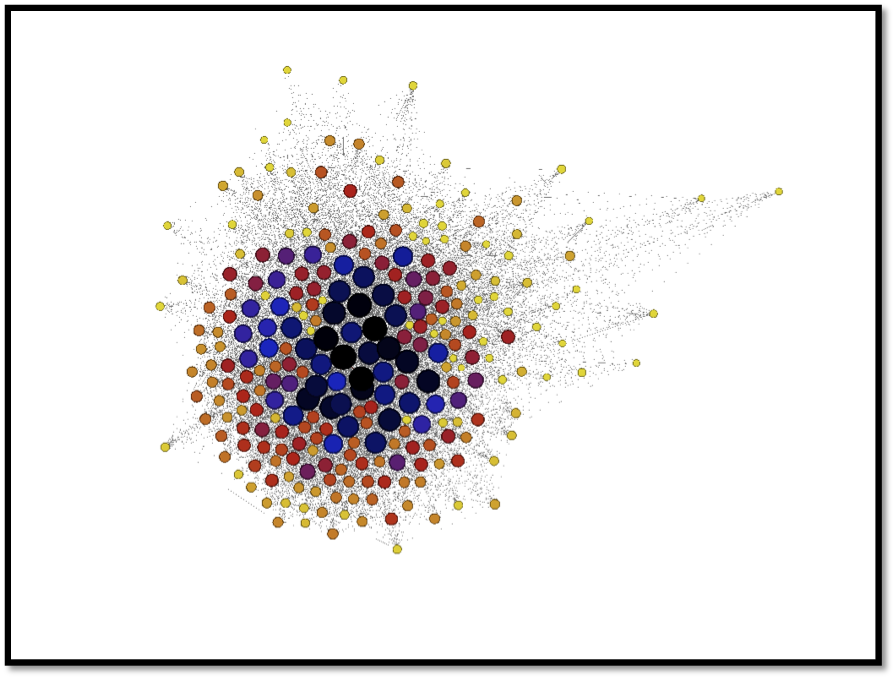
\includegraphics[scale=0.7]{img/7/grafo12}
\caption{Relaciones entre etiquetas.
\label{fig:grafo12}}
\end{figure}

Otro grafo más simplificado se muestra en la figura~\ref{fig:grafo14}, con las siguientes características:
\begin{itemize}
\item    El grafo tiene 21 nodos y 86 aristas.
\item    Los nodos están escalados según su grado nodal (número de relaciones con otras etiquetas).
\item    Las aristas están escaladas según su peso (número de ocurrencias de esa relación).
\item    Aparecen 2 comunidades en el grafo: color del nodo (turquesa y rojo).
\item    El grado nodal medio del grafo es 8,19.
\item    Sólo hay 1 componente conexa.
\end{itemize}

\begin{figure}
\centering
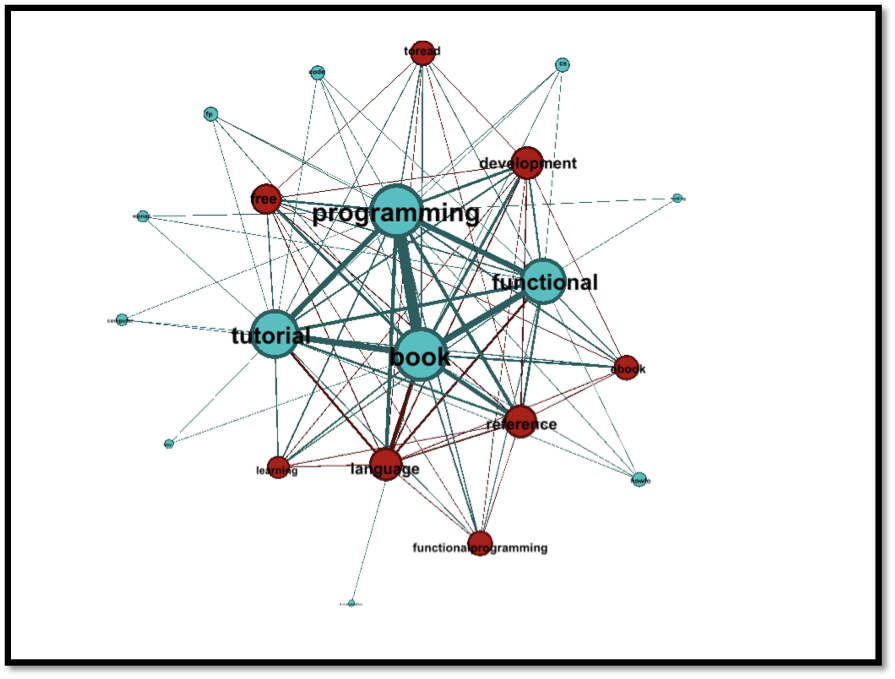
\includegraphics[scale=0.7]{img/7/grafo14}
\caption{Relaciones entre etiquetas (simplificado).
\label{fig:grafo14}}
\end{figure}

La generación de este nodo simplemente es un proceso de simplificación en el que se eliminan los nodos con menor grado nodal con respecto al grafo anterior.





\subsection{Relaciones entre usuarios (por lenguaje común).}

Este grafo presenta las relaciones entre los {\bf usuarios} del sistema, en función de su {\bf lenguaje común}; es decir, el número de etiquetas comunes con otros usuarios.

\subsubsection{Representación.}

Este grafo tiene como puntos de partida:

\begin{itemize}
\item    Los nodos corresponden a los usuarios del sistema.
\item    El peso de los nodos es el tamaño del lenguaje de dicho nodo (usuario); es decir, el número de etiquetas que usa dicho usuario.
\item    Las aristas representan relaciones entre dos usuarios (dos nodos). Esta relación existirá cuando posean algún lenguaje común; es decir, que compartan alguna etiqueta (aunque dicha etiqueta no esté en los mismos enlaces para ambos). Otra forma de verlo sería decir que existe una arista entre dos usuarios cuando la interesección de sus conjuntos de etiquetas es no vacía.
\item    El peso de las aristas es el número de etiquetas que forman parte de dicha intersección.
\end{itemize}

\subsubsection{Resultado.}

El grafo obtenido tiene las siguientes características:

\begin{itemize}
\item    El número de nodos es 4259.
\item    El número de aristas es 6844837.
\item    El grado nodal máximo del grafo es 4178; es decir, existe un usuario cuyo lenguaje (conjunto de etiquetas) contiene alguna etiqueta en común con el lenguaje de otros 4178 usuarios.
\item    El grado nodal medio del grafo es 1607.1465
\item    El peso nodal máximo es 238; es decir, un usuario que ha etiquetado con 238 etiquetas diferentes, y ese es el número máximo de nuestro sistema.
\item    El peso nodal medio es $7.3575954$.
\item    El peso de arista máximo es 64; es decir, existe un par de usuarios cuya intersección de lenguajes (conjunto de etiquetas comunes) está formada por 64 etiquetas, y este par de usuarios es el que tiene una intersección más grande.
\item    El peso medio de las aristas es de $2.0418215$
\item Los nodos más destacables son \emph{{\bf 75: airlab.am}} ($peso=238$), \emph{{\bf 47: MC Andre}} ($peso=192$), \emph{{\bf 11: Tang Tong}} ($peso=167$), \emph{{\bf 104: Matthew}} ($peso=141$) y \emph{{\bf 3002: timcowlishaw}} ($peso=134$).
\item Las aristas más destacables son \emph{{\bf 75-104}} ($peso=64$), \emph{{\bf 11-75}} ($peso=56$), \emph{{\bf 11-104}} ($peso=53$), \emph{{\bf 75-1659}} ($peso=46$) y \emph{{\bf 75-115}} ($peso=43$). Estas aristas expresan los IDs de los usuarios en el sistema.
\end{itemize}

\subsubsection{Simplificación del grafo.}

Se llevan a cabo las siguientes tareas para simplificar el grafo:

\begin{itemize}
\item    Un primer proceso de filtrado consistirá en eliminar todos aquellos nodos cuyo peso nodal sea menor que el peso nodal medio del grafo (que es $7.3575954$). Esta operación, además de eliminar estos nodos, elimina también todas las aristas cuyo origen o destino tiene a este nodo. Recuérdese que el peso nodal se corresponde con el tamaño del lenguaje del usuario representado por dicho nodo; es decir, el número de etiquetas diferentes que ha usado en el etiquetado. Por tanto, con este filtrado se eliminarán a todos aquellos usuarios cuyo lenguaje tenga menos de 8 etiquetas diferentes.
\item    Un segundo proceso de filtrado consistirá en eliminar todas aquellas aristas cuyo peso sea menor que el peso medio de arista del grafo (que es $2.0418215$). Recuérdese que el peso de arista se corresponde con el tamaño del lenguaje común de un par de usuario (usuario del nodo origen y usuario del nodo destino); es decir, el número de etiquetas distintas que son usadas por ambos usuarios. Por tanto, con este filtrado se eliminarán a todos aquellos pares de usuarios cuyo lenguaje común tenga menos de 3 etiquetas comunes.
\item A continuación, se repetirá el proceso de filtrado de aristas que no superen el nuevo peso medio de arista obtenido tras el proceso anterior. Este nuevo valor es $4.144222$.
\item Finalmente, se eliminan las aristas menos significativas (aquellas con menor peso), y todos los nodos que pasen a tener grado nodal 0.
\end{itemize}


\subsubsection{Grafo resultante.}

El grafo resultante se muestra en la figura~\ref{fig:grafo33}. Algunas características de este grafo son:

\begin{itemize}
\item    Los nodos son usuarios, se incluye el nombre de cada usuario.
\item    El tamaño del nodo está escalado según su grado nodal; es decir, según el número de otros usuarios con los que tiene relación. Su nombre está igualmente escalada.
\item    Las aristas son relaciones entre dos usuarios.
\item    La anchura de las aristas está escalada según su peso; es decir, según el tamaño del lenguaje común que representa dicha aristas.
\item    Los nodos y las aristas están coloreados según las comunidades a las que pertenecen, existiendo 4 comunidades diferentes.
\end{itemize}

\begin{figure}
\centering
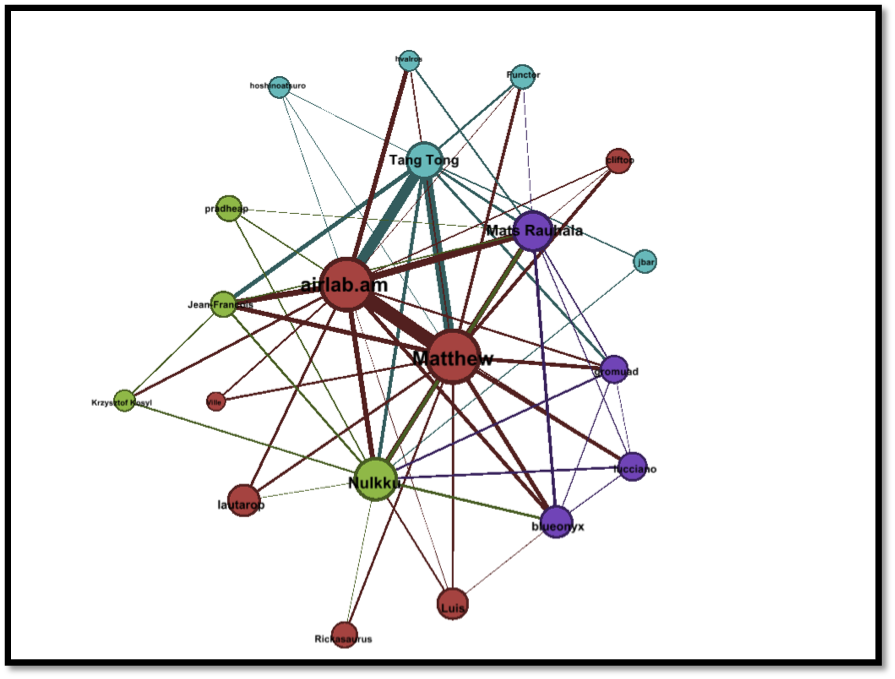
\includegraphics[scale=0.7]{img/7/grafo33}
\caption{Relaciones entre usuarios (por lenguaje común).
\label{fig:grafo33}}
\end{figure}








\subsection{Relación entre usuarios (por contextos comunes).}

Este grafo, muy similar al anterior, presenta las relaciones entre los {\bf usuarios} del sistema, en función de los {\bf contextos comunes} que tienen entre ellos; es decir, el número de enlaces comunes con otros usuarios.

\subsubsection{Representación.}

Este grafo tiene como punto de partida:

\begin{itemize}
\item    Los nodos corresponden, igual que en el grafo anterior, a los usuarios del sistema.
\item    El peso de los nodos es el tamaño del contexto de dicho nodo (usuario); es decir, el número de enlaces que tiene etiquetado dicho usuario.
\item    Las aristas representan relaciones entre dos usuarios (dos nodos). Esta relación existirá cuando posean algún contexto común; es decir, que compartan algún enlace (aunque dicho enlace no tenga la misma etiquetación para ambos). Otra forma de verlo sería decir que existe una arista entre dos usuarios cuando la interesección de sus conjuntos de enlaces es no vacía.
\item    El peso de las aristas es el número de enlaces que forman parte de dicha intersección.
\end{itemize}

\subsubsection{Resultado.}

El grafo obtenido tiene las siguientes características:
\begin{itemize}
\item    El número de nodos es 4259. Igual que para el grafo anterior.
\item    El número de aristas es 616708. Se observa que este número es mucho menor que en el grafo anterior, ya que es más difícil que dos usuarios compartan enlaces a que compartan etiquetas.
\item    El grado nodal máximo del grafo es 1877; es decir, existe un usuario cuyo contexto (conjunto de enlaces) contiene algún enlace en común con el lenguaje de otros 1877 usuarios.
\item    El grado nodal medio del grafo es $144.80113$.
\item    El peso nodal máximo es 111.
\item    El peso nodal medio es $2.3944588$
\item    El peso de arista máximo es 11; es decir, existe un par de usuarios cuya intersección de contexto (conjunto de enlaces comunes) está formada por 11 enlaces, y este par de usuarios es el que tiene una intersección más grande.
\item    El peso medio de las aristas es de $1.0205121$.
\item Los nodos más destacables que en el caso anterior: \emph{{\bf 75: airlab.am}} ($peso=238$), \emph{{\bf 47: MC Andre}} ($peso=192$), \emph{{\bf 11: Tang Tong}} ($peso=167$), \emph{{\bf 104: Matthew}} ($peso=141$) y \emph{{\bf 3002: timcowlishaw}} ($peso=134$).
\item Las aristas más destacables son: \emph{{\bf 104-105}} ($peso=11$), \emph{{\bf 104-331}} ($peso=9$), \emph{{\bf 11-104}} ($peso=8$), \emph{{\bf 104-215}} ($peso=7$) y \emph{{\bf 104-796}} ($peso=7$).
\end{itemize}

\subsubsection{Simplificación y grafo resultante.}

Al igual que en el proceso anterior, se han eliminado las aristas menos significativas (según su peso), para que la representación sea amigable, dejando únicamente visibles en el siguiente grafo las aristas más significativas del sistema. En este proceso de filtrado se han eliminado todas aquellas aristas con peso menor que 5; es decir, se han eliminado todos los pares de usuarios que comparten menos de 5 enlaces en su contexto común. Obviamente, se han eliminado también los nodos que, tras la eliminación de estas aristas, han quedado con grado nodal igual a 0; es decir, sin relaciones con ningún otro usuario.

También se han escalado los nodos según su grado nodal (y también los nombres de éstos), las aristas según su peso, y se han coloreado tanto nodos como aristas en función de las comunidades obtenidas.

El grafo resultante se puede ver en la figura~\ref{fig:grafo42}.

\begin{figure}
\centering
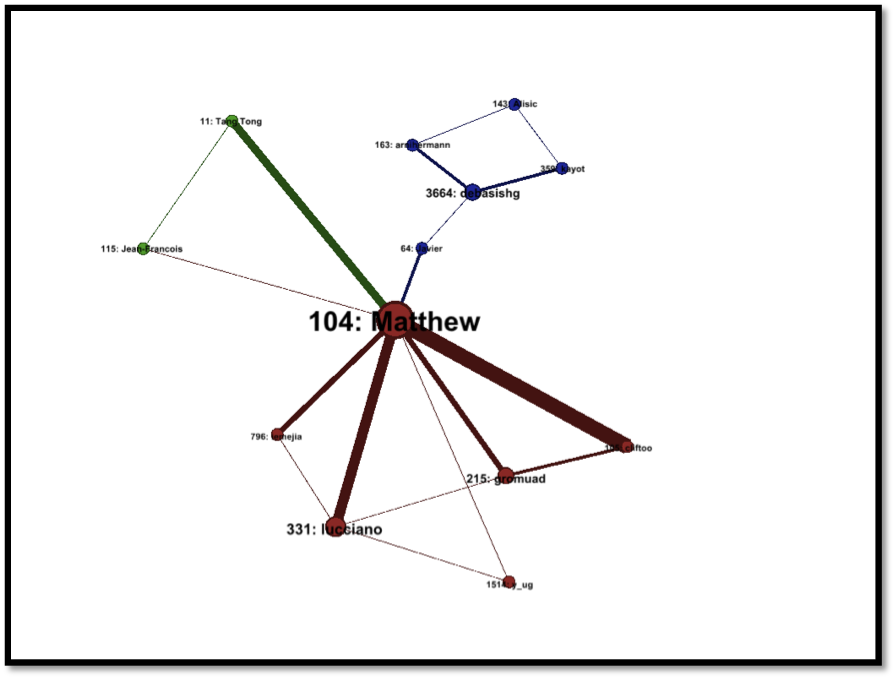
\includegraphics[scale=0.7]{img/7/grafo42}
\caption{Relaciones entre usuarios (por contexto común).
\label{fig:grafo42}}
\end{figure}


\section{Ejecución del SMA.}

Como se comentó en el capítulo~\ref{cap:capitulo6}, se ha realizado una ejecución del sistema con umbrales iguales o superiores a 3. Para optimizar las ejecuciones, cada ejecución se ha ceñido a calcular aquellas conciliaciónes de un valor concreto; es decir, que sólo se realizarán conciliación de conceptos entre aquellos usuarios que compartan exactamente el número de objetos marcados por el valor de \emph{umbral}. Sin embargo, todos los resultados se almacenan en una base de datos de forma conjunta, de forma que se puedan sacar conclusiones a posteriori.

De esta forma, se ha realizado un pequeño script, en el que se obtienen los siguientes resultados (ver tabla~\ref{fig:resultados}), tanto totales, como separados por los diferentes posibles valores de \emph{umbral}. Hay que indicar que este proceso realiza un cálculo del número de conceptos y el número de implicaciones de cada contexto encontrado. Estos contextos son, precisamente, los contextos comunes resultados de alguna conciliación tras la ejecución del SMA. Los datos que se adjuntan se refieren a estos valores por cada contexto conciliado.

Finalmente, hay que indicar que no se ha realizado con umbrales inferiores a 3 por cuestiones de implementación, tal como se comentaba en el capítulo anterior.

\begin{figure}
\centering
{ \scriptsize
\begin{tabular}{|l|c|c|c|c|c|c|c|c|c|c|}
\hline
& Total 
&\begin{sideways} Umbral=3 \end{sideways} 
&\begin{sideways} Umbral=4 \end{sideways} 
&\begin{sideways} Umbral=5 \end{sideways} 
&\begin{sideways} Umbral=6 \end{sideways} 
&\begin{sideways} Umbral=7 \end{sideways} 
&\begin{sideways} Umbral=8 \end{sideways} 
&\begin{sideways} Umbral=9 \end{sideways} 
&\begin{sideways} Umbral=10 \end{sideways} 
&\begin{sideways} Umbral=11 \end{sideways} 
 \\ \hline

Nº Conciliaciones & 663 		& 561 	& 75 		& 15 		& 7 		& 2 		& 1 		& 1 & 0 &  1   \\ \hline
Media Objetos 	& $33.546$ 	& $28.742$ & $52.76$ & $76.667$ & $71.714$ & 87 	& 144 	& 92 & - &  98   \\ \hline
Total Objetos & 22241 		& 16124 	& 3957 	& 1150 	& 502 	& 174 	& 144 	& 92 &-  &  98 \\ \hline
Máx Objetos & 144 			& 130 	& 117 	& 138 	& 86 		& 97 		& 144 	& 92 & - &  98   \\ \hline
Media Lenguaje & $9,413$ 		& $8.234$ 	& $13.2$ 	& $24$ 	& 12 		& 30 		& 53 		& 38 & - &  37   \\ \hline
Total Lenguaje & 6241 		& 4619	& 990	& 360	& 84 		& 60 		& 53 		& 38 & - &  37   \\ \hline
Máx Lenguaje & 64 			& 43 		& 42 		& 64 		& 26 		& 38 		& 53 		& 38 & - &  37   \\ \hline
Media Conceptos & $6.092$ & $5.365$ 	& $7.867$ 	& $15.333$ & 10 	& $26.5$ 	& 32 		& 25 & - &  29   \\ \hline
Total Conceptos & 4039 	& 3010 	& 590 	& 230 	& 70 		& 53 		& 32 		& 25 & - &  29   \\ \hline
Máx Conceptos & 40 		& 40 		& 26 		& 38 		& 23 		& 32 		& 32 		& 25 & - &  29   \\ \hline
Media Implicaciones & $9.75$ & $7,957$ & $14.653$ & $34,467$ & $15.143$ & $45.5$ & 80 	& 51 & - &  56   \\ \hline
Total Implicaciones & 6464 	& 4464 	& 1099 	& 517 	& 106 	& 91 		& 80 		& 51 & - &  56   \\ \hline
Máx Implicacioens & 114 	& 71 		& 58 		& 114 	& 38 		& 50 		& 80 		& 51 & - &  56   \\ \hline
\end{tabular}
}
\caption{Resultados de la Ejecución del SMA
\label{fig:resultados}
}

\end{figure} 






\section{Resultados estadísticos y Conclusiones.}

En la figura~\ref{fig:estNConc} se puede observar una gráfica del número de conciliaciones en función del umbral. En esta gráfica se observa un decrecimiento exponencial del número de conciliaciones a medida que aumenta el umbral. Esto tiene sentido ya que el número de usuarios que quieren conciliar su conocimiento con otros usuarios aumentará a medida que se reduce este umbral de objetos comunes. En los umbrales más altos, se ve como el número de conciliaciones tiende a cero. Añadir, además, que no se adjuntan datos para las conciliaciónes con umbral igual a 0, 1 y 2; porque no se ha implementado en el sistema.

%\begin{figure}
%%\centering
%
%\begin{minipage}[b]{0.42\linewidth}
%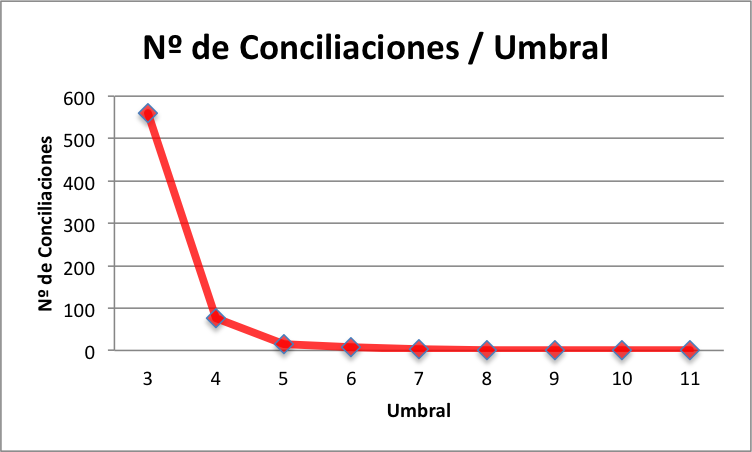
\includegraphics[scale=0.47]{img/7/est_nconciliaciones}
%\end{minipage}
%\hspace{0.1cm}
%\begin{minipage}[b]{0.42\linewidth}
%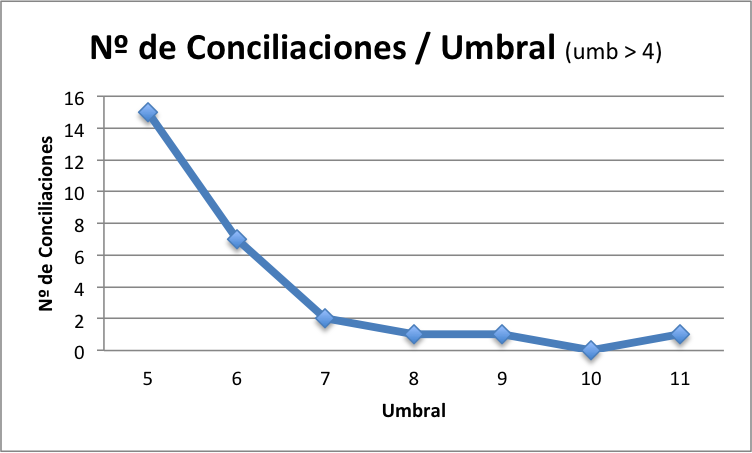
\includegraphics[scale=0.56]{img/7/est_nconciliaciones2}
%\end{minipage}
%
%\caption{Número de conciliaciones por umbral.
%\label{fig:estNConc}}
%\end{figure}

\begin{figure}
\centering

\begin{minipage}[b]{0.45\linewidth}
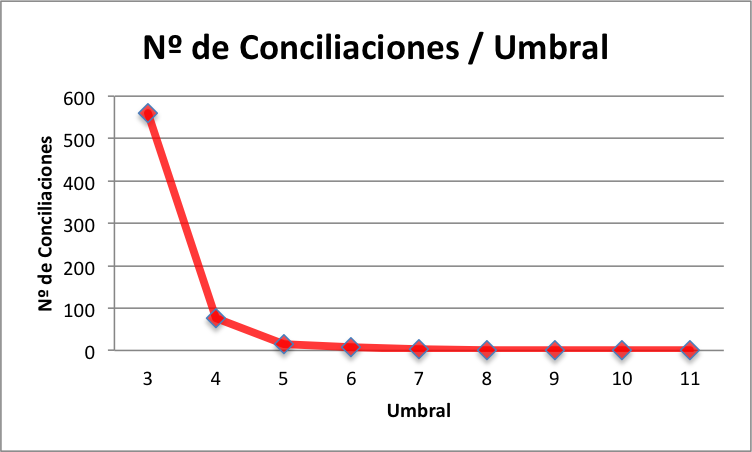
\includegraphics[scale=0.5]{img/7/est_nconciliaciones}
\end{minipage}
\hspace{0.3cm}
\begin{minipage}[b]{0.45\linewidth}
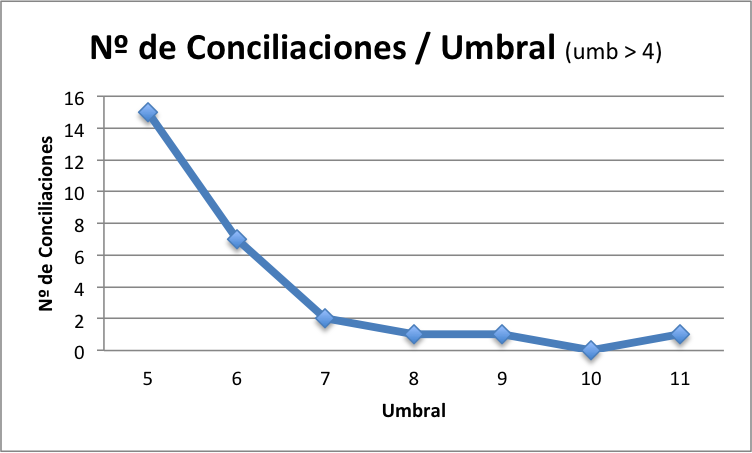
\includegraphics[scale=0.5]{img/7/est_nconciliaciones2}
\end{minipage}

\caption{Número de conciliaciones por umbral.
\label{fig:estNConc}}
\end{figure}

En la figura~\ref{fig:estObj} se puede observar una doble gráfica sobre el número de objetos comunes y el número de atributos comunes por contexto conciliado en función del umbral. Estos valores son la media de todos los contextos conciliados para dicho umbral. Se ve como inicialmente, los contextos generados poseen muy pocos objetos y atributos, por lo que son contextos muy pobres. Esto se explica ya que cuando dos usuarios tienen pocos objetos en común, es también probable que su lenguaje común sea reducido; y por tanto, la conciliación apenas genere nuevas sugerencias. En cambio, a medida que los umbrales aumentan; es decir, a medida que los usuarios comparten más objetos, se observa una tendencia de contextos más ricos en cuanto a número de objetos y número de atributos. Sin embargo, lo más importante es notar esta tendencia, ya que los valores numéricos no son significativos puesto que el número de contextos conciliados no es muy elevado.

\begin{figure}
\centering
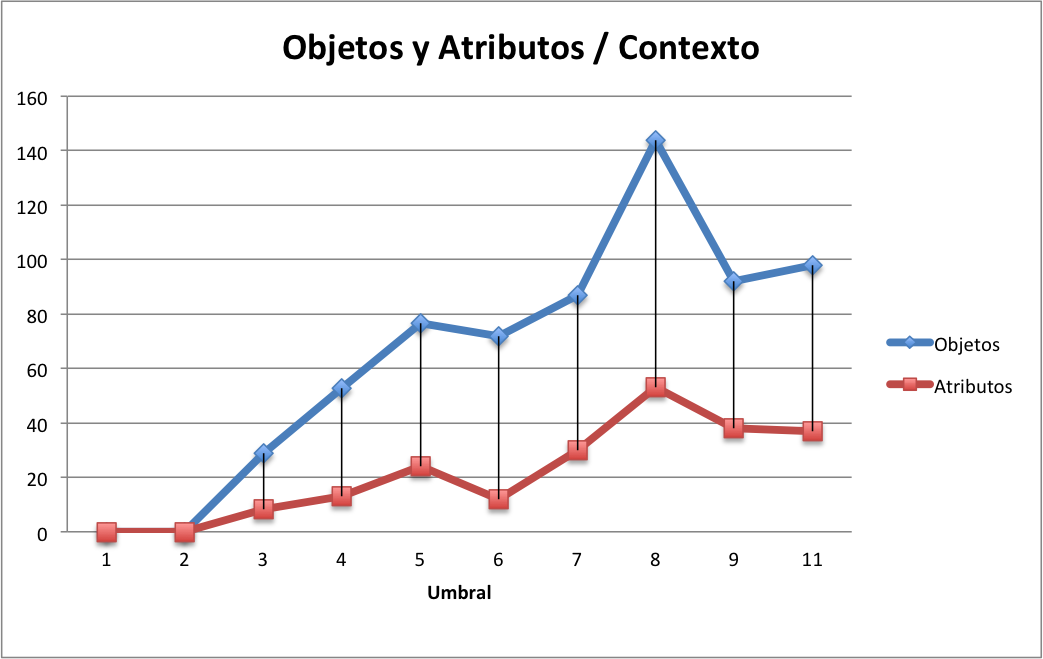
\includegraphics[scale=0.75]{img/7/est_nobj}
\caption{Número medio de Objetos y Atributos por Contexto conciliado según Umbral.
\label{fig:estObj}}
\end{figure}

Finalmente, en la figura~\ref{fig:estconceptos} se puede observa una doble gráfica sobre el número de conceptos y el número de implicaciones por contexto conciliado en función del umbral. Estos valores son la media de todos los contextos conciliados para cada uno de estos umbrales. Igual que en el caso anterior, se obseva una tendencia positiva en cuanto al crecimiento de número de conceptos y número de implicaciones generados por contexto conciliado a medida que aumenta el umbral; es decir, a medida que los pares de usuarios que concilian su conocimiento comparte un mayor número de enlaces. Es interesante destacar que en los últimos umbrales se producen algunas desviaciones en esta tendencia. Esto es debido a que el número de conciliaciones es muy reducido (1 o 2 según el caso), por lo que no representan una muestra representativa para tomar valores exactos. Sin embargo, muestran perfectamente esta tendencia creciente.

\begin{figure}
\centering
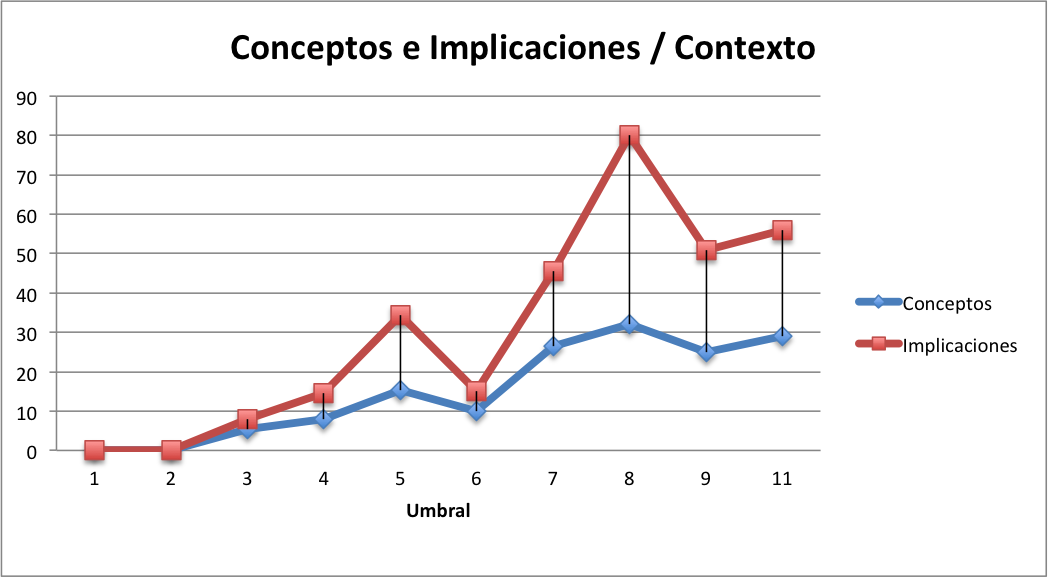
\includegraphics[scale=0.75]{img/7/estconceptos}
\caption{Número medio de Conceptos e Implicaciones por Contexto conciliado según Umbral.
\label{fig:estconceptos}}
\end{figure} % Resultados
\chapter{Conclusiones y Trabajo Futuro.}\label{cap:capitulo8}

En este capítulo se explican las conclusiones finales de este trabajo, y se comentarán algunas líneas de trabajo futuro.

\section{Conclusiones.}

En este trabajo se ha presentado un método para conciliar el conocimiento global de un Sistema de Etiquetado (SE). Este método está basado en la tecnología multiagente, y se ha llevado a cabo con una implementación realizada en JADE (\cite{jade}). El sistema de etiquetado elegido ha sido Delicious (\cite{delicious}); concretamente se ha elegido un subconjunto de datos de Delicious, obtenido a partir de la etiqueta {\bf haskell} (ver capítulo~\ref{cap:capitulo5}).

La solución realizada (ver capítulo~\ref{cap:capitulo6}) es un SMA basado en negociación entre agentes, de forma que a medida que transcurre la ejecución de este SMA, los agentes (que representa a los usuarios del SE) negocian con otros agentes con los que quieren conciliar su conocimiento. Esto va generando diferentes contextos conciliados entre pares de usuarios, que representan el conocimiento común. Estos contextos se almacenan en una base de datos, guardando los identificadores de ambos usuarios, los objetos (enlaces) y sus atributos (etiquetas) que forman parte del contexto, y también el número de objetos que comparten ambos usuarios (que en este trabajo hemos llamado \emph{{\bf umbral}}). Es trivial obtener una representación de este contexto utilizando las herramientas de ConExp (\cite{conexp}), nos centraremos en obtener el Retículo de Conceptos (formales) y las Bases Stem que representan este Contexto común.

Finalmente, se han tomado muestras de los resultados obtenidos (ver capítulo~\ref{cap:capitulo7}), en los que se observa una relación inversa entre el umbral (o número de objetos que dos usuarios comparten) y el número de conciliaciones que se producen para dicho umbral; es decir, cuanto mayor es el umbral, existen menos parejas de usuarios para conciliar su conocimiento. Sin embargo, la relación es directa entre el umbral y el tamaño de los contextos, medido en el número de objetos y atributos generado, y en el número de conceptos e implicaciones obtenidos; es decir, a medida que crece el umbral, los contextos generados, aunque sean menos, son más ricos, pues tienen un mayor número de objetos (enlaces), atributos (etiquetas), conceptos generados e implicaciones obtenidas. Estos resultados se justifican trivialmente porque:
\begin{itemize}
	\item A medida que se aumenta el umbral, el número de conciliaciones es menor, puesto que habrá un mayor número de pares de usuarios que compartan pocos enlaces.
	\item A medida que se aumenta el umbral, el tamaño de los contextos conciliados es mayor, puesto que si un par de usuarios comparte muchos enlaces es previsible que también tengan un lenguaje común (o número de atributos comunes) grande (aunque no siempre se da esta circunstancia), y por tanto, también es previsible que la conciliación genere un gran número de sugerencias. El resultado es, por tanto, un contexto conciliado grande.
\end{itemize}

Es interesante destacar que partiendo de un conjunto de datos relativamente grande (compuesto por 4259 usuarios, 2427 etiquetas, 3028 enlaces y 45079 tuplas), se producen un total de 663 conciliaciones con $umbral \geq 3$; es decir con usuarios que comparten al menos 3 enlaces.

De este total, 561 de ellas se realizan cuando únicamente comparten 3 enlaces (y no más); esto representa el $84.62$\% del total de conciliaciones. Además, es interesante ver las características de estos contextos conciliados que tiene de media\footnote{Se ha aproximado al límite entero superior} 29 objetos, 9 atributos, 6 conceptos y 8 implicaciones. Aunque el número de objetos (y relativamente también el número de atributos) es suficientemente grande, los contextos generados son muy \emph{pobres} ya que el número de conceptos e implicaciones es muy bajo. Hay que recordar que en el ejemplo que se ilustraba en el capítulo~\ref{cap:capitulo2}, con un contexto de únicamente 5 objetos y 3 atributos (mucho más pequeño que en este caso) se obtiene 6 conceptos (que ya supera la media obtenida) y 1 implicación. En conclusión, la mayoría de los contextos obtenidos son muy pobres.

De las 102 conciliaciones restantes (conciliaciones entre usuarios que comparten 4 o más enlaces), que representan el $15.38$\% del total, 75 de ellas se producen cuando únicamente comparten 4 enlaces. Esto representa un $73.53$\% relativo, y un $11.31$\% total. De nuevo, vuelven a ser un número bastante grande en comparación con el número de conciliaciones para umbrales superiores. Sin embargo, poco a poco se comienza a observar una mejoría en cuanto a la calidad de los contextos obtenidos, que están formados, de media, por 53 objetos, 14 atributos, 8 conceptos y 15 implicaciones.

Finalmente hay que indicar que los cálculos totales para el conjunto completo de contextos conciliados obtienen, de media, contextos formados por 34 objetos, 10 atributos, 7 conceptos y 10 implicaciones. Estos números se sitúan precisamente entre los umbrales 3 y 4.

En conclusión, a medida que se reduce el umbral aumenta el número de conciliaciones, pero los contextos generados son más pobres. El umbral mínimo que se ha establecido en la implementación de este trabajo ha sido 3, debido a que: (1) apenas se conseguían contextos significativos; y (2) los problemas de implementación que conlleva la ejecución de un SMA con umbrales tan bajos, en los que tienen que convivir muchos agentes, y la mayoría de ellos tiene una carga computacional alta.

Por otra parte, es interesante destacar el criterio que se ha utilizado para seleccionar que pares de usuarios que realizan conciliación es el {\bf número de objetos que comparten}. Este criterio se ha tomado por decisión no sistemática debido a un análisis no formal, cuya conclusión es que si el propio algoritmo filtra un lenguaje común entre pares de usuarios (conjunto de atributos comunes), un buen criterio para seleccionar estos pares es elegir el número de objetos comunes. La justificación es que, previsiblemente, el contexto obtenido tenga un número de objetos aceptable, que podría ser más bajo si muchos objetos son filtrados por no estar etiquetados con ninguna etiqueta del lenguaje común. Normalmente, este caso se produce cuando comparten pocos objetos. Sin embargo, esto no deja de ser una previsión, por lo que existen casos excepcionales que no cumplen esta regla. En la sección siguiente, veremos algunas líneas de trabajo futuro en este sentido.

Por último, es interesante hacer mención a los umbrales que no se han ejecutado; es decir, 0\footnote{Entiéndase que $umbral=0$ si no comparten ningún enlace.}, 1 y 2. En estos casos, las soluciones obtenidas no merecen la pena para el esfuerzo que conlleva en tareas de implementación. Este trabajo pretendía estudiar analíticamente los resultados producidos por la Conciliación en un Sistema de Etiquetado, y para ello se ha elegido un conjunto de datos cuyo tamaño es pequeño en comparación con el volumen de datos de un SE real. Estos resultados son muy interesantes y establecen un campo de trabajo que puede favorecer la navegación semántica en sistemas basados en folksonomías. En cambio, es interesante hacer notar que el número de conciliaciones producidas para umbrales relativamente altos\footnote{Estos umbrales deben ser mayores con conjuntos de datos de mayor volumen.} es muy pequeño, consecuencia de que el conjunto de prueba tiene también un volumen de datos relativamente pequeño. Sin embargo, en sistemas reales donde el volumen de datos sea exponencialmente mayor, este número de conciliaciones también crecerá, y por tanto, nos enfrentaremos a los mismos problemas que con estos umbrales pequeños (0, 1 y 2). En el capítulo~\ref{cap:capitulo6}, se comentaron algunas soluciones de implementación para solventar estos aspectos, que se comentan de forma más específica en la siguiente sección.




\section{Trabajo futuro.}

En esta sección, vamos a distinguir algunas líneas de trabajo futuro, divididas en varios ámbitos de aplicación: Investigación, Implementación y Aplicación.

\subsection{Investigación.}

En este apartado, vamos a describir algunas líneas de investigación; ya sea bien porque no se conoce concretamente los resultados esperados introduciendo ciertos cambios en el sistema, o bien porque son consecuencia de los resultados ya obtenidos. Veamos estas líneas:

\begin{itemize}

	\item Se ha visto las diferentes conclusiones obtenidas según el criterio utilizado para elegir a los pares de usuarios. Sería interesante investigar el comportamiento del sistema en base a otros criterios. Se deduce un criterio muy simple que es precisamente seleccionar los pares en función del tamaño de su lenguaje común; es decir, del número de atributos comunes. También sería interesante restringir este lenguaje común a aquellas etiquetas que ambos usuarios usan en el mismo enlace. Por otra parte, también se pueden buscar criterios más complejos. En el grafo~\ref{fig:grafo42}, se expresaban las relaciones más importantes entre los usuarios más relevantes. Otras posibles criterios pueden estar basados en distancias entre nodos de este grafo, o comunidades de usuarios. En cualquier de los criterios anteriores, es interesante contrastar los resultados que se obtengan con los de este trabajo.

	\item Por ahora, sólo se ha implementado la Conciliación de conocimiento por pares de usuarios. Sin embargo, también se deduce una tarea que puede ser muy interesante: ¿cuál es el conocimiento compartido por un sistema completo, o por un grupo de usuarios? En esta línea, sería interesante investigar cuales son los resultados si se concilia varios contextos conciliados, para obtener el conocimiento conciliado de múltiples usuarios.

	\item En la misma línea del punto anterior, en \cite{jaschke} se introducen los \emph{triconceptos} como modelo de conceptualizaciones compartidas por grupos de usuarios. Este elemento podría ser interesante para trabajar con el conocimiento conciliado de todos ellos. 

	\item En el ámbito del Análisis Formal de Conceptos, sería interesar investigar nuevas técnicas para recalcular los Retículos de Conceptos y sus Bases Stem asociadas en contextos dinámicos; es decir, en contextos que continuamente están cambiando. En la implementación actual, un cambio en el contexto implica tener que recalcular estos elementos para el nuevo contexto una vez modificado. Sería interesante descubrir métodos para reducir estos cálculos, puesto que es de suponer que una pequeña variación en el contexto, generará pequeñas variaciones en los retículos y en las bases Stem.

	\item En este trabajo, el conjunto de datos de prueba se ha parametrizado en función de su volumen. Sin embargo; un aumento en el volumen de datos no implica que las conciliaciones obtenidas sean más ricas, ni que se produzcan en un número.  Sería interesante introducir nuevas medidas del conjunto de datos de entrada para establecer un criterio de \emph{calidad}. Esto puede ser útil para estudiar diferentes criterios de aplicación en función de las características del conjunto de datos de entrada. Además, puede ser interesante para ofrecer comparativas acerca de los resultados obtenidos para diferentes datos de entrada.

	\item En la misma línea del punto anterior, sería interesante establecer un criterio de evaluación de los resultados obtenido. En este trabajo nos hemos ceñido a presentar el volumen de estos datos (en cuanto a medias, máximos y totales sobre el número de objetos, atributos, conceptos e implicaciones de los contextos obtenidos). Sería interesante conseguir una representación gráfica en forma de grafo, por ejemplo, que nos permita comparar distintos resultados en función del criterio seleccionado o del conjunto de datos de entrada.

\end{itemize}






\subsection{Implementación.}

En este apartado vamos a ver algunas líneas de trabajo futuro que están especialmente relacionadas con cuestiones técnicas de implementación. Algunas de estas cuestiones se introdujeron en las nota de implementación del capítulo~\ref{cap:capitulo6}; y otras se tratan de nuevas cuestiones que aún no se han tratado.

\begin{itemize}

	\item En el capítulo~\ref{cap:capitulo6} se comentaba la problemática de la ejecución del SMA cuando en la ejecución de éste participan un gran número de agentes. Recordemos que cada agente representa a un usuario del Sistema de Etiquetado. El hecho de que haya un gran número de agentes conviviendo en la plataforma se debe a que la restricción que se ha impuesto para que dos usuarios concilien su conocimiento (o no) es una restricción débil, permitiendo, de esta forma, que exista un gran número de usuarios implicados en este proceso. Además, cuando este número de conciliaciones es elevado, no es únicamente elevado el número de agentes, sino que también es elevado el número de interacciones entre estos agentes, los cuales pretenden conciliar su conocimiento con muchos otros agentes. Esto provoca un problema técnico por colapso en los recursos. Para solventar este problema, se propone una ejecución distribuida en varias máquinas, de forma que el agente Control, que se encarga de poner en marcha y gestionar todo el proceso, y que sea capaz de distribuir a los agentes en diferentes contenedores. La arquitectura de JADE (\cite{jade}) permite crear fácilmente esta estructura en la que, teniendo una única plataforma, existan diversos contenedores en los que se encuentren los agentes. La solución consistiría, básicamente, en que cada contenedor se encontrara en una máquina distinta, y se repartieran los agente proporcionalmente según estos contenedores. Esta solución no deja de ser una primera aproximación, pues si el volumen de datos del problema creciera exponencialmente, situación que podría ocurrir si se implantara este SMA en un Sistema de Etiquetado real (en este trabajo sólo se ha utilizado un conjunto muy pequeño de datos en comparación con el volumen de los sistemas reales); entonces también tendría que crecer mucho el número de máquinas que acogiesen a los contenedores pertinentes, llegando a ser inviable en ciertos casos.

	\item En la misma línea que el punto anterior, se podría establecer un mecanismo de reparto de carga dinámico entre un número fijo de contenedores, de forma que el (o los) agente(s) de control pudieran repartir a los usuarios del SMA en los diferentes contenedores según el volumen de carga computacional de cada uno de los usuarios en cada momento. Esta solución solventa el problema del crecimiento ilimitado del número de contenedores; sin embargo, tampoco es una solución definitiva, pues es posible que el contenedor oportuno se siga colapsando debido a una carga de trabajo demasiado grande y que no pueda asumir. Además, surge un nuevo problema debido al cuello de botella que se produce en la tarea de reparto de carga, y todos los problemas que derivan de éste: posible colapso, errores fatales en caso de que el agente muera y no sea capaz de recuperarse, etc.

	\item Sin ser incompatible con las soluciones anteriores, otra solución que se plantea es crear varios agentes de control, de forma que se reduzcan los efectos del cuello de botella de este agente, y además, solventar las consecuencias de posibles muertes de alguno de estos agentes, en la que el resto de agentes asumirían el trabajo del agente ya muerto, y el sistema podría continuar su ejecución normalmente.

	\item Paralelamente a la solución del reparto de carga dinámica, y no por ello incompatible con ésta, se podría llevar a cabo una solución en la que se limitara el número de conciliaciones que se producen en cada momento. Primeramente habría que establecer un número máximo de conciliaciones simultáneas, de forma que se garantice la buena ejecución del sistema, evitando posibles colapso por consumo total de los recursos disponibles Una vez hecho esto, existen varias estrategias para cumplir esta limitación. Pongamos dos ejemplos: sistema de pizarra, y agente distribuidor. La primera estrategia consistiría, \emph{a grosso modo}, en una pizarra accesible desde cualquier agente, de forma que todos ellos pudieran consultar la información allí escrita, y que además, todos pudieran modificar dicha información. De esta forma, cada agente, antes de iniciar una conciliación, debería consultar esta pizarra para decidir si es posible comenzar esta conciliación; y en caso de no ser posible, esperar hasta que pueda comenzar. La segunda estrategia consiste en establecer un agente encargado de dar permiso o negarlo a los usuarios que soliciten comenzar una conciliación; de forma que siempre se cumpla la limitación del número de conciliaciones simultáneas.

	\item Existen ocasiones en los que, durante la ejecución de los comportamientos del agente, se producen excepciones y su ejecución se aborta. Estas excepciones conllevan, generalmente, la muerte del agente. Se propone un sistema de copia de seguridad y restauración del agente en caso de que se produzcan estas excepciones. Una posible solución es capturar adecuadamente todas estas excepciones, y antes de que el agente muera, pueda guardar su estado y reiniciarse. En ciertos casos, quizás sea necesario que esta tarea se complemente con un agente restaurador encargado de esta misión.

	\item A lo largo de este trabajo se ha hablado de la solución propuesta como una función secuencial que, dado unos datos de entrada, devuelve unos resultados. En sistemas reales esta concepción no es viable, debido a que el gran volumen de datos y el incremento de éstos paulatinamente implica que la tarea probablemente nunca termine (excepto en aquellos casos que se imponga una restricción muy fuerte, y por tanto, los resultados obtenidos sean muy pobres). Una línea de trabajo interesante sería plantear este sistema con un funcionamiento atemporal, de forma que durante su ejecución produzca ciertos resultados, intentado priorizar aquellos resultados que a priori se consideren más importantes.

	\item Finalmente, y como se explicaba en la sección anterior, puede ser interesante estudiar en qué términos, un retículos (y sus implicaciones asociadas) cambian en función de pequeños cambios en el contexto, sin tener que recalcularlo todo de nuevo. Sería interesante implementar estas técnicas antes de aplicar el sisteman a un entorno dinámico al que se incorporen nuevos datos en cada instante.


\end{itemize}





\subsection{Aplicación.}

Finalmente, en esta sección vamos a ver algunas de las líneas de trabajo futuro que pueden ser interesantes para implantar este sistema en un Sistema de Etiquetado real.

\begin{itemize}

	\item A lo largo de todo este capítulo se han visto las diferencias entre el conjunto de datos utilizado y un conjunto de datos de un Sistema de Etiquetado real. La diferencia en cuanto a volúmenes de datos es abismal. Por tanto, sería interesante analizar los resultados obtenidos en un sisteman en el que los usuarios compartan muchos más enlaces y más atributos. Por ejemplo, sería muy interesante saber si, a partir de cierto umbral (de objetos o atributos compartidos, o cualquier otro), el tamaño de los contextos conciliados crece de forma exponencial (en lugar de crecer de forma lineal como ocurre en este trabajo). Para saber si esta circunstancia ocurre, no queda más remedio que llevar a cabo la ejecución con un volumen de datos mucho más grande.

	\item En la introducción de este trabajo se comentaban algunas de las principales motivaciones de este trabajo, que no son otras que establecer un conocimiento común entre usuarios para otros usos futuros, como navegación entre usuarios, búsquedas autocompletadas con la información semántica que otros usuarios puedan aportar, sugerencias de nuevos etiquetado, etc... Sería interesante aplicar alguna de estas ideas a los resultados conseguidos con este trabajo, para ver su verdadera utilidad y comparar su comportamiento frente a otras herramientas y utilidades que existen actualmente en el mercado.

	\item Como se remarca en \cite{algoritmo}, es necesario seguir trabajando en las contextualizaciones de grupos de usuario, para extraer conocimiento (semántico) a partir de éstas. Una extensión del algoritmo básico con el fin de encontrar ontologías consesuadas por todos los usuarios (o grupos amplios de ellos), debe ser una línea fundamental de trabajo desde el punto de vista de la aplicación semántica.

\end{itemize}






 % Conclusiones
\begin{thebibliography}{99}

\addcontentsline{toc}{chapter}{Bibliografía.}

\bibitem{alonso} Alonso-Jiménez, J.A., Aranda-Corral, G.A., Borrego-Díaz, J., Fernández-Lebrón,
M.M., Hidalgo-Doblado, M.J. (2008). Extending Attribute Exploration by Means of Boolean Derivatives. In: Proc. 6th Int. Conf. on Concept Lattices and Their Applications. CEUR Workshops Proc., p. 433. 

\bibitem{algoritmo} Aranda-Corral, G.A., Borrego-Díaz, J. (2010). Reconciling Knowledge in Social Tagging Web Services. Lecture Notes in Computer Science, 6077(1), 101-121.

\bibitem{mowento} Aranda-Corral, G.A., Borrego-Díaz, J., Gómez-Marín, F. (2009). Toward Semantic Mobile Web 2.0 through Multiagent Systems. In: Håkansson, A., Nguyen, N.T., Hartung, 
R.L., Howlett, R.J., Jain, L.C. (eds.) KES-AMSTA 2009. LNCS, vol. 5559, pp. 400–409. Springer, Heidelberg.

\bibitem{blondel} Blondel, V.D., Guillaume, J.L., Lambiotte, R., Lefebvre, E. (2008). Fast unfolding of communities in large networks. Journal of Statistical Mechanics: Theory and Experiment, Vol. 2008, No. 10.

\bibitem{brooks} Brooks, C.H., Montanez, N. (2006). Improved annotation of the blogosphere via autotagging and hierarchical clustering. In WWW 06. Proceedings of the 15$^{th}$ international conference on World Wide Web, (pp.625-632.). New York: ACM Press.  

\bibitem{afc} Ganter, B., Wille, R. (1999). Formal Concept Analysis - Mathematical Foundations. Springer, Heidelberg.

\bibitem{golder} Golder, S., Huberman, B.A. (2006). The structure of collaborative tagging systems. Journal of Information Science 32(2), 98-208.

\bibitem{gruber} Gruber, T. (2007). Ontology of Folksonomy: A Mash-up of Apples and Oranges. Int'l. Journal on Semantic Web \& Information Systems 3(2).

\bibitem{halpin} Halpin, H., Valentin R., and Hana S. (2006). The dynamics and semantics of collaborative tagging. Proceedings of the 1$^{st}$ Semantic Authoring and Annotation Workshop (SAAW06). 

\bibitem{jaschke} Jäschke, R., Hotho, A., Schmitz, C., Ganter, B., Stumme, G. (2008). Discovering shared conceptualizations in folksonomies. Journal of Web Semantics 6(1), 38–53.

\bibitem{kim} Kim, H.-L., Scerri, S., Brslin, J., Decker, S., Kim, H.-G. (2008). The state of the art in tag ontologies: A semantic model for tagging and folksonomies. In: International Conference on Dublin Core and Metadata Applications, Berlin, Germany.

\bibitem{knerr} Knerr, T. (2006). Tagging ontology-towards a common ontology for folksonomies. \url{http:// tagont.googlecode.com/files/TagOntPaper.pdf}.

\bibitem{mathes} Mathes, A. (2004). Folksonomies - Cooperative Classification and Communication Through Shared Metadata. \url{http://www.adammathes.com/academic/computer-mediated-communication/folksonomies.html}

\bibitem{mika} Mika, P. (2005). Ontologies Are Us: A unified model of social networks and semantics. Proceedings of the 4$^{th}$ International Semantic Web Conference, ISWC 2005, Galway, Ireland, (pp. 522-536). Berlin, Heidelberg: Springer.  

\bibitem{rowley} Rowley, J. (1995). Organizing Knowledge. 2$^{\mbox{\scriptsize nd}}$ Ed. Brookfield, VT: Gower.

\bibitem{shirky} Shirky, C. (2005). Ontology is Overrated: Categories, Links and Tags. \url{http://www.shirky.com/writtings/ontology_overrated.html}

\bibitem{smith} Smith, G. (2007). Tagging: People-Powered Medatada for the Social Web. First. New Riders Publishing, Indianapolis.

\bibitem{tanaka} Tanaka, J.W., Taylor, M. (1991) . Object categories and expertise: Is the basic level in the eye of the beholder? Cognitive Psychology 23(3), 457–482.

\bibitem{van} Van Damme, C., Hepp, M., Siorpaes, K. (2007). FolksOntology: An Integrated Approach for Turning Folksonomies into Ontologies. In: ESWC 2007 workshop Bridging the Gap between Semantic Web and Web 2.0, May 2007, pp. 57–70.

\bibitem{weick} Weick, K.E., Sutcliffe, K.M., Obstfeld, D. (2005). Organizing and the Process of Sense\-making. Organization Science 16(4), 409–421.

\bibitem{yeung} Yeung, C.M.A., Gibbins, N., Shadbolt, N. (2009). Contextualising Tags in Collaborative Tagging Systems. In: Proceedings of the 20th ACM Conference on Hypertext and 
Hypermedia.


\bibitem{conexp} ConExp: \url{http://conexp.sourceforge.net/}

\bibitem{delicious} Delicious: \url{http://www.delicious.com/}

\bibitem{dot} Notación DOT: \url{http://www.graphviz.org/Documentation.php}

\bibitem{fipa} FIPA (Foundation for Intelligent Physical Agents): \url{http://www.fipa.org/}

\bibitem{gephi} Gephi: \url{http://gephi.org/}

\bibitem{jade} JADE (Java Agent Development Framework): \url{http://jade.tilab.com/}

\end{thebibliography}









%%  Apendices
%%%%%%%%%%%%%%%%%%%%%%%%%%%%%%%%%%%%%%%%%%%%%%%%%%%%%%%%%%%%%%%%%%%%%%

%\appendix
%\include{apendice}  % Puedo poner la ontología OSMV y la arquitectura de OW

%%  Bibliografia
%%%%%%%%%%%%%%%%%%%%%%%%%%%%%%%%%%%%%%%%%%%%%%%%%%%%%%%%%%%%%%%%%%%%%%
%\newpage
%\addcontentsline{toc}{chapter}{Bibliografía}
%\bibliographystyle{alpha}
%\bibliography{bibliografia.tex}

\end{document}

